% \documentclass[print]{gescons} % Quando for enviar para a gráfica
\documentclass[a4paper]{gescons}

\magazinename  {GENSCONS}
\magazinetheme {GENSCONS}
\magazinevolume{7}
\magazineissue {2025}

\usepackage[export]{adjustbox} % \adjincludegraphics com Clip/trim

% --- codificação e idioma (pdfLaTeX) ---
\RequirePackage[T1]{fontenc}        % encoding T1 -> hifeniza melhor em PT
\RequirePackage[utf8]{inputenc}     % seu .tex está em UTF-8
\RequirePackage[brazil]{babel}      % regras de hifenização PT-BR
%\emergencystretch=2em               % evita overfull hbox

\begin{document}
    % \frontpage{images/capa}{15}{15}
    %\% frontpage{images/capa.pdf}{15}{15}
    %\frontpage{images/capa.pdf}{0}{0}

    \tableofcontents

    \documentclass{gescons}

\genre {Editorial}
\author{Amanda Vieira}
\title{20 anos de Publicação Interassistencial: Passado, Presente e Futuro da Editares}

\begin{document}
    \makeentrevistatitle
    %\maketitle

    %\fullwidthimage{fields}{b}

    \coverart{back/editorial}
    %\coverart{../fundo-generico.png}

    \begin{multicols}{2}

%\begin{center}
%    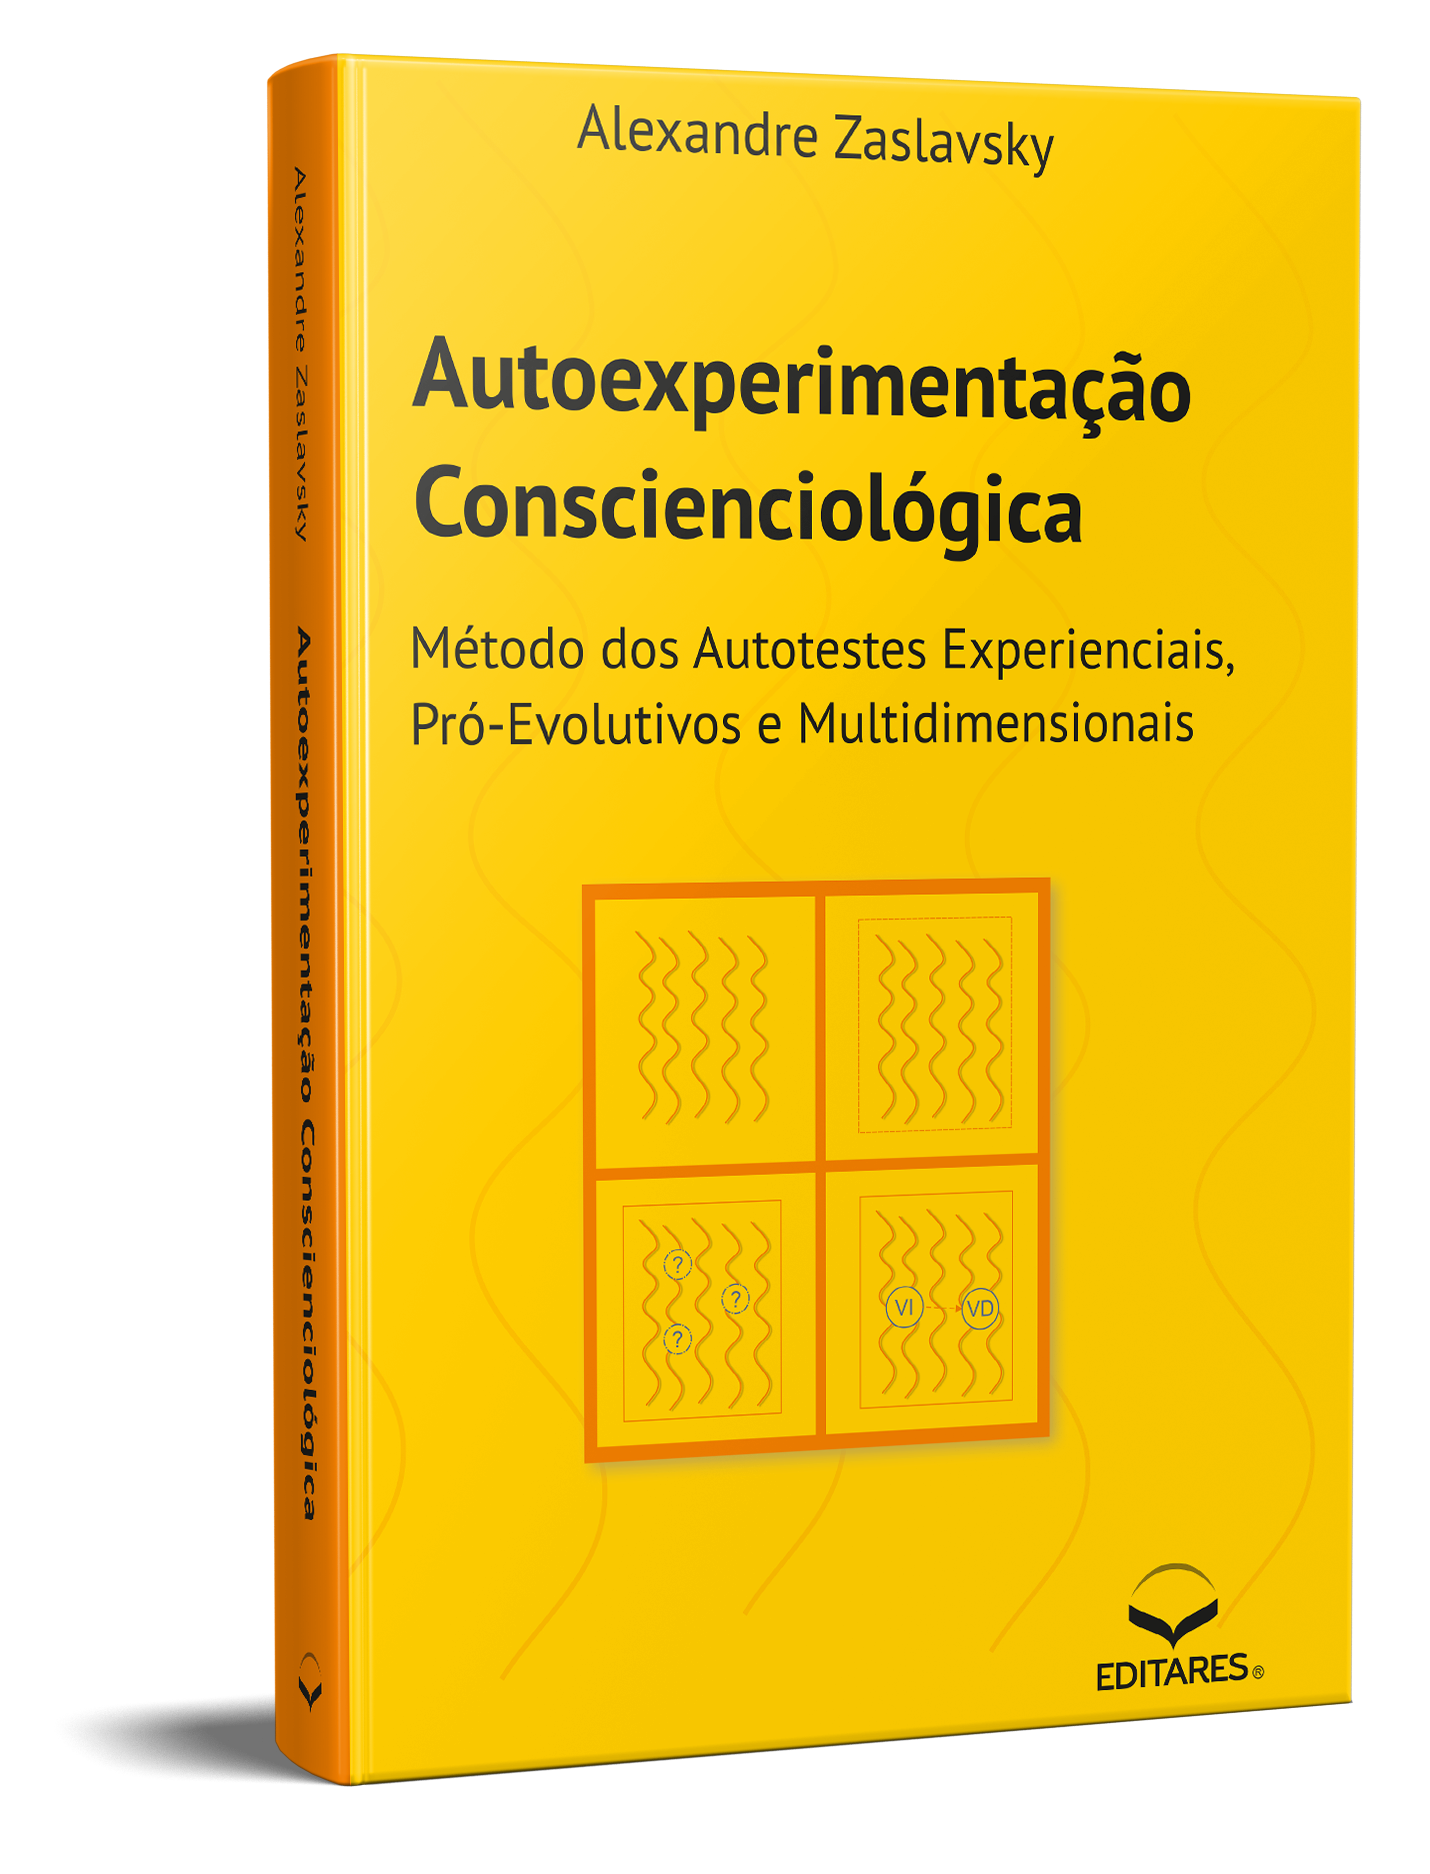
\includegraphics[width=4cm]{articles/entrevista/mockups/Alexandre-Zas.png}
%\end{center}

Em 2024, a Editares completou 20 anos de dedicação à publicação técnico-científica de obras conscienciológicas. Duas décadas de trabalho tarístico, construídas por muitas mãos, em que cada autor, revisor, diagramador, conselheiro, voluntário e leitor fez parte de um mesmo propósito: \textbf{expandir o esclarecimento e favorecer a evolução das consciências por meio da escrita.}

Celebrar essa história significa reconhecer o valor do esforço coletivo. Desde os primeiros livros publicados até os mais recentes lançamentos, cada obra representa um marco de interassistência, registrando aprendizados, reflexões e contribuições para o desenvolvimento da Conscienciologia e para a maxiproéxis grupal.

Esta edição da Revista Gescons propõe um olhar integrado sobre a trajetória da Editares: passado, presente e futuro se encontram para inspirar novos desafios e conquistas. É um convite para pensar no que já realizamos juntos e, principalmente, no que ainda podemos alcançar coletivamente.

Na primeira seção, apresentamos \textbf{resumo do biênio} com os acontecimentos mais relevantes da Editares entre 2023 e 2024: a conquista da Certificação Institucional da UNICIN, a participação no Congraçamento das ICs, a distribuição internacional de materiais no Japão e na Europa, as atualizações do fluxo editorial e os números que refletem nossa produção recente. Um destaque especial vai para a listagem completa dos voluntários atuais, organizados por equipes de trabalho, valorizando quem faz a Editares acontecer.

Na segunda seção, trazemos \textbf{atualizações} e novidades institucionais: a criação da Escola de Editores, voltada à formação e qualificação de novos voluntários; as novas estratégias de marketing; a nova revista científica da Editares para expansão da especialidade Editoriologia e Publicaciologia; a reativação da parceria com o IIPC para ampliar a venda de livros; e os grupos de trabalho com a UNICIN, responsáveis por repensar processos comerciais e editoriais.

Por fim, na terceira seção, apresentamos os \textbf{lançamentos de 2024 e 2025,} com obras que ampliam o debate técnico e aprofundam a pesquisa conscienciológica.

Mais do que celebrar o passado, esta edição propõe \textbf{um olhar para o futuro.} Queremos inspirar novos autores, atrair mais voluntários e consolidar práticas editoriais cada vez mais qualificadas e interassistenciais. Seguimos firmes no propósito de transformar ideias em livros, livros em esclarecimento e esclarecimento em evolução.

Agradecemos a todos os voluntários, autores, leitores e parceiros que fazem parte desta história. Que os próximos anos sejam ainda mais produtivos, lúcidos e interassistenciais.

Boa leitura!



%\begin{center}
%    %  trim={<left> <lower> <right> <upper>}
%    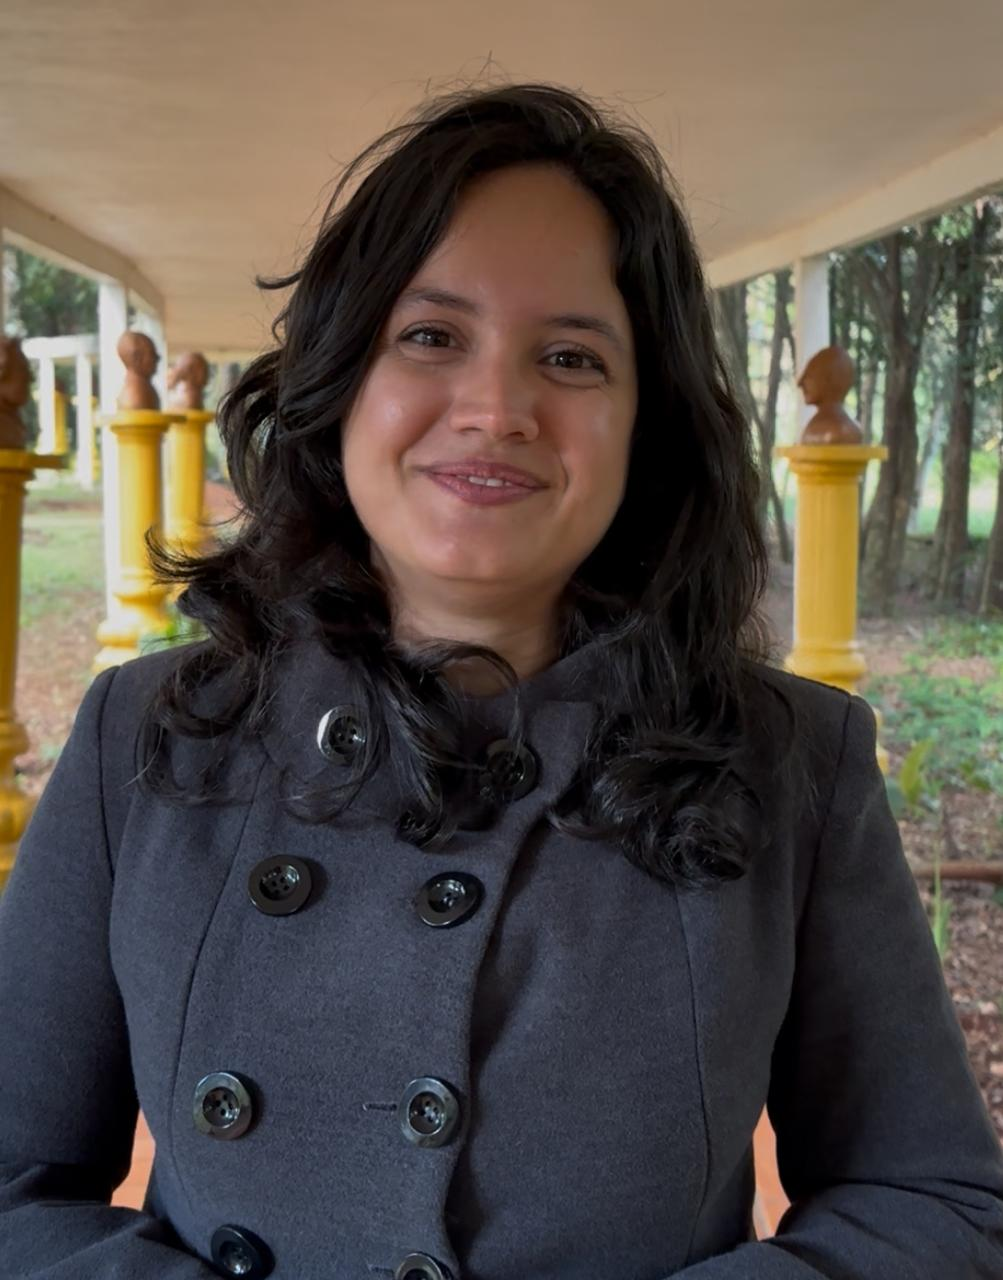
\includegraphics[width=8cm,trim={0 200 0 70},clip]{articles/inicial/imagens/Amanda.jpeg}
%\end{center}

%\begin{pullquote}
%``A escrita de uma obra conscienciológica é uma oportunidade evolutiva inigualável.''
%\end{pullquote}

        
    \end{multicols}

\begin{figure}[h] % [htbp] are placement options (here, top, bottom, page)
\centering % Centers the image and caption
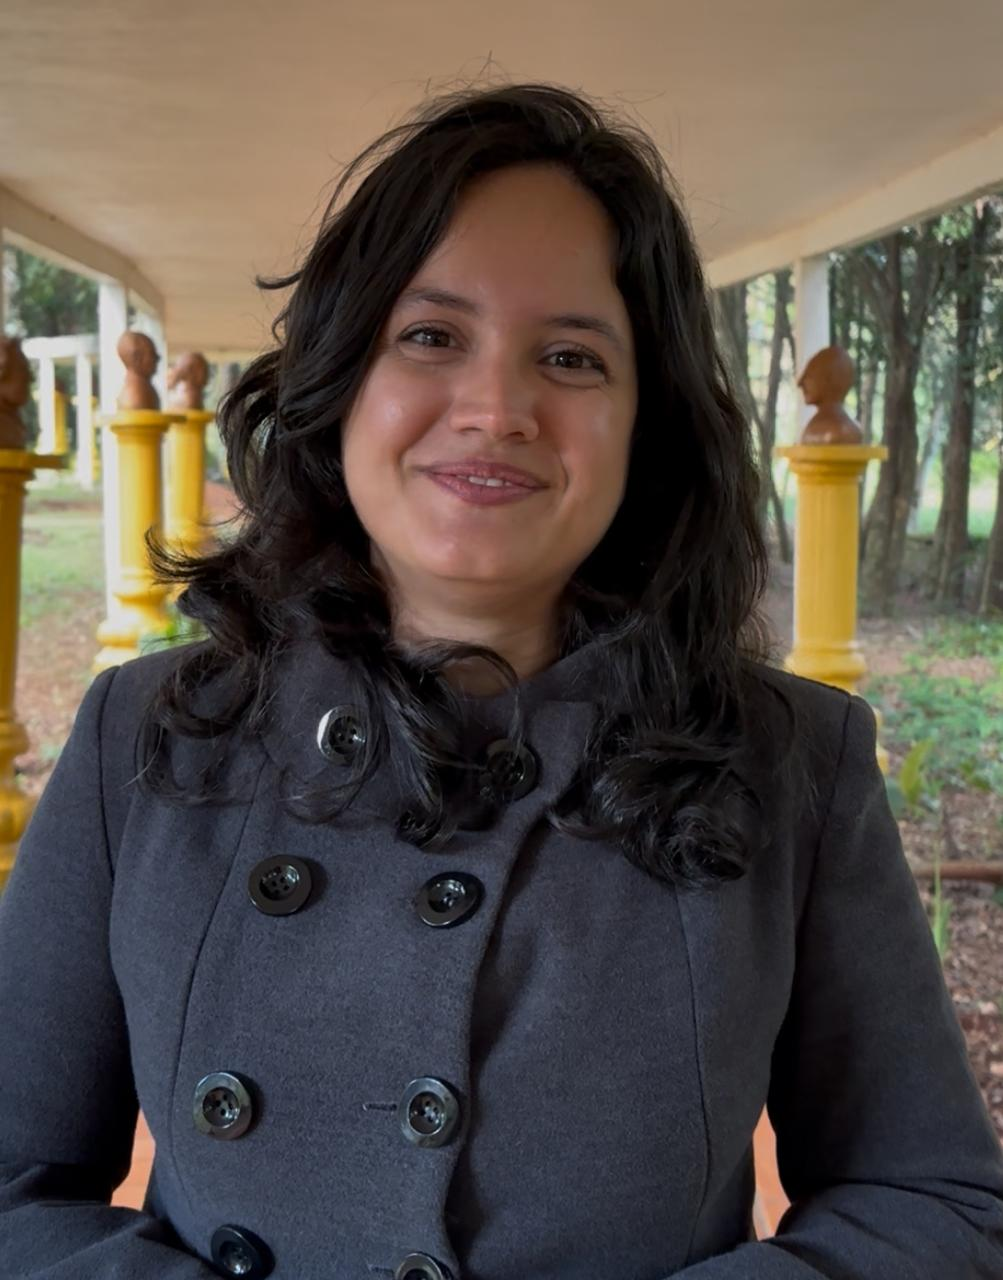
\includegraphics[width=5cm,trim={0 200 0 70},clip]{articles/inicial/imagens/Amanda.jpeg}
\caption*{Editora desta Edição} % The caption text
\end{figure}

\end{document}

    
    \genre{}
    \title {Resumo do Biênio}
    \author{}
    \authorrole{}
    \makecovertitle{articles/fundo-generico.png}{}

    \documentclass{gescons}

\genre {Resumo do Biênio}
\author{Ana Claudia Prado e Magda Stapf Amancio}
\title{Gestão 2024-2025: Entrevista com as Coordenadoras}

\begin{document}
    \makeentrevistatitle
    %\maketitle

    %\fullwidthimage{fields}{b}

    %\coverart{back/editorial}
    \coverart{../fundo-generico.png}

    \begin{multicols}{2}

%\begin{center}
%    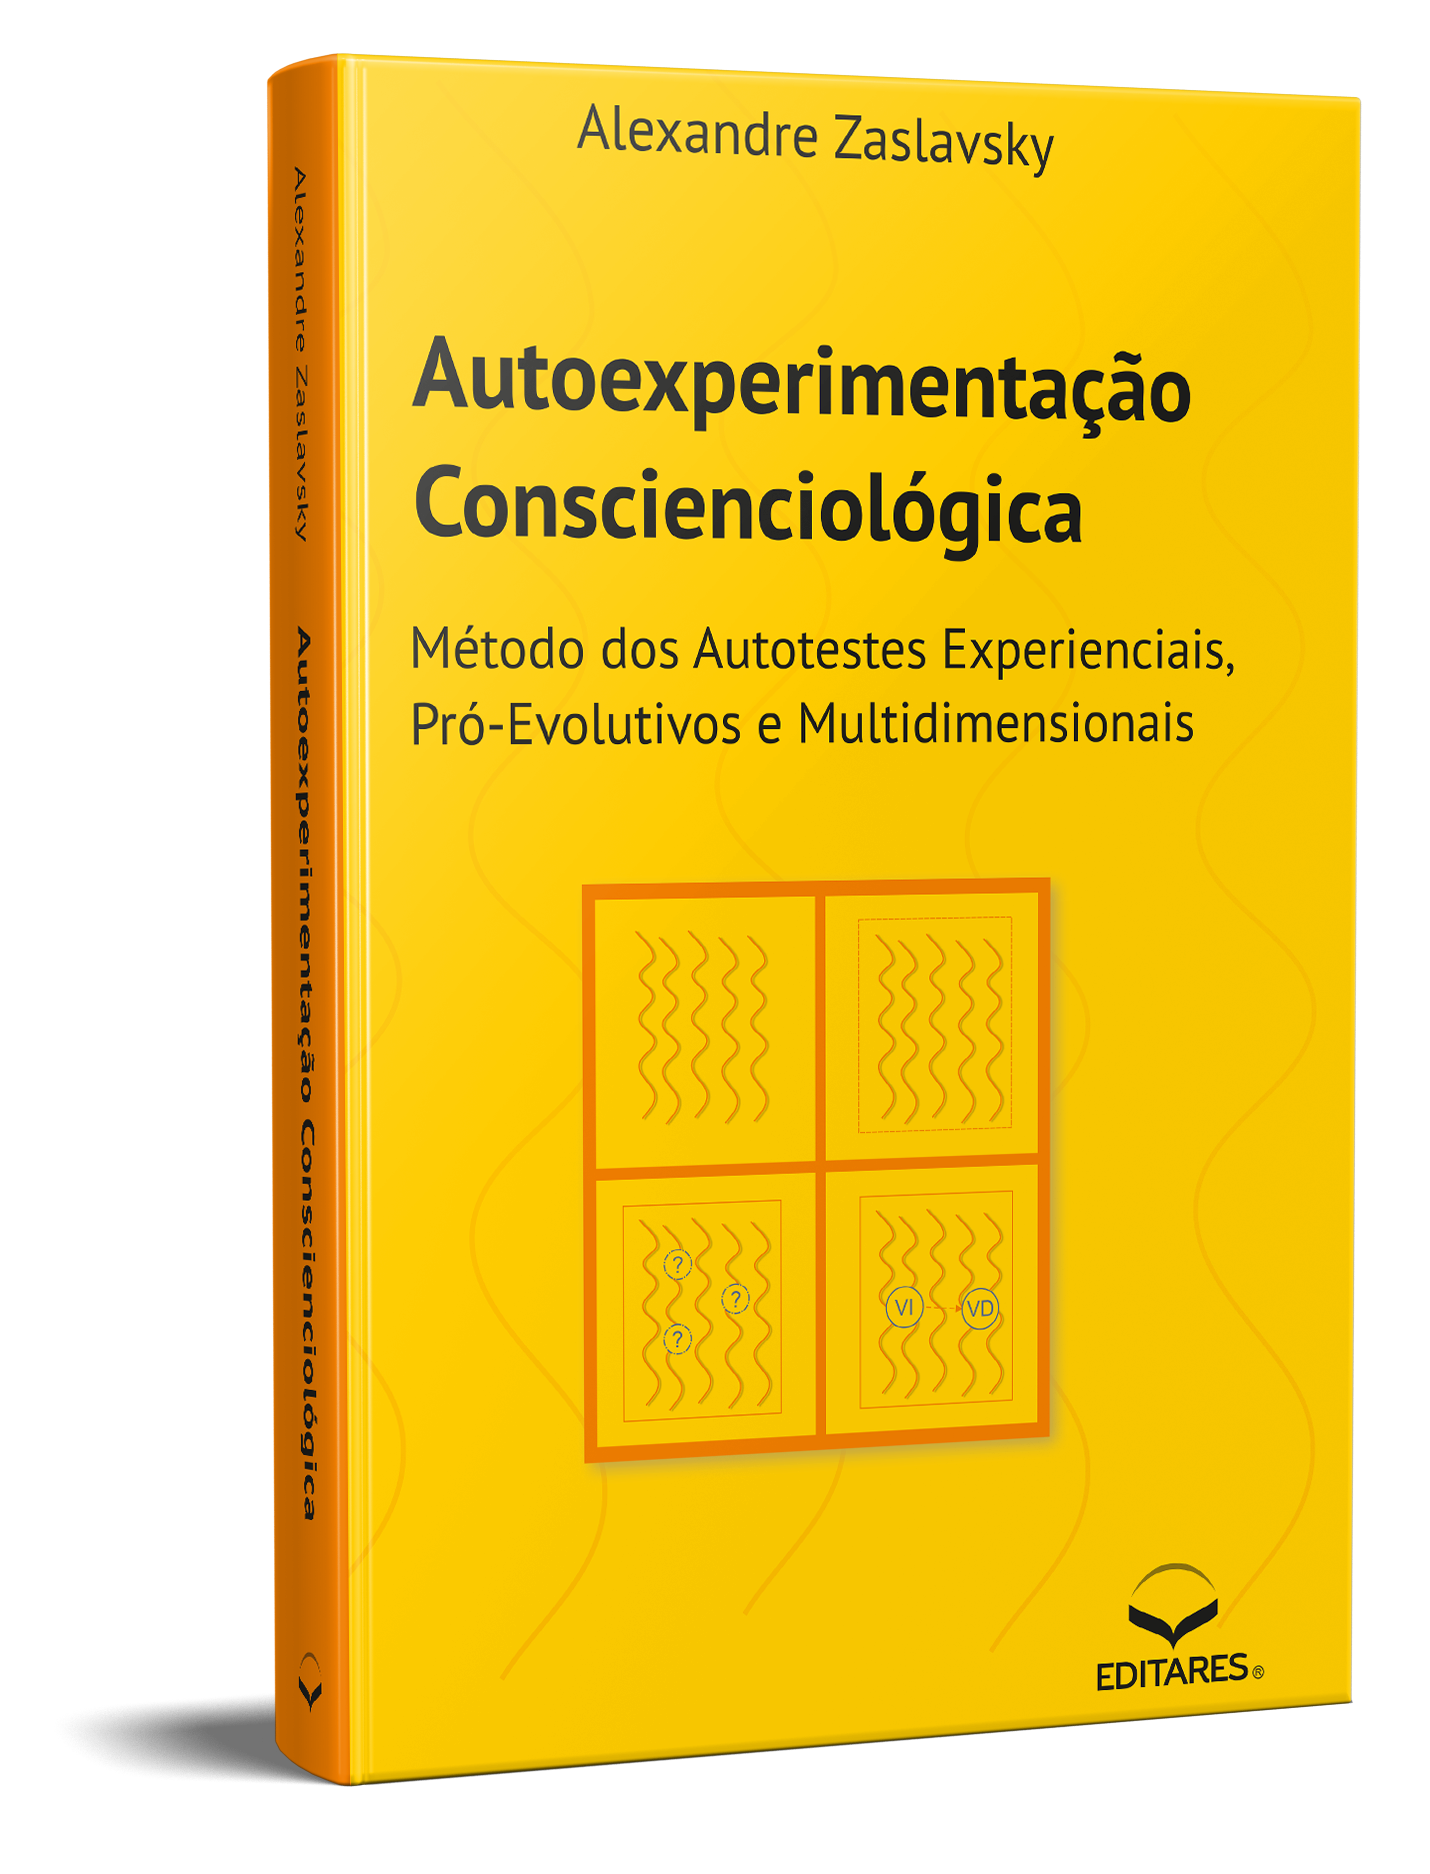
\includegraphics[width=4cm]{articles/entrevista/mockups/Alexandre-Zas.png}
%\end{center}

    \begin{center}
        %  trim={<left> <lower> <right> <upper>}
        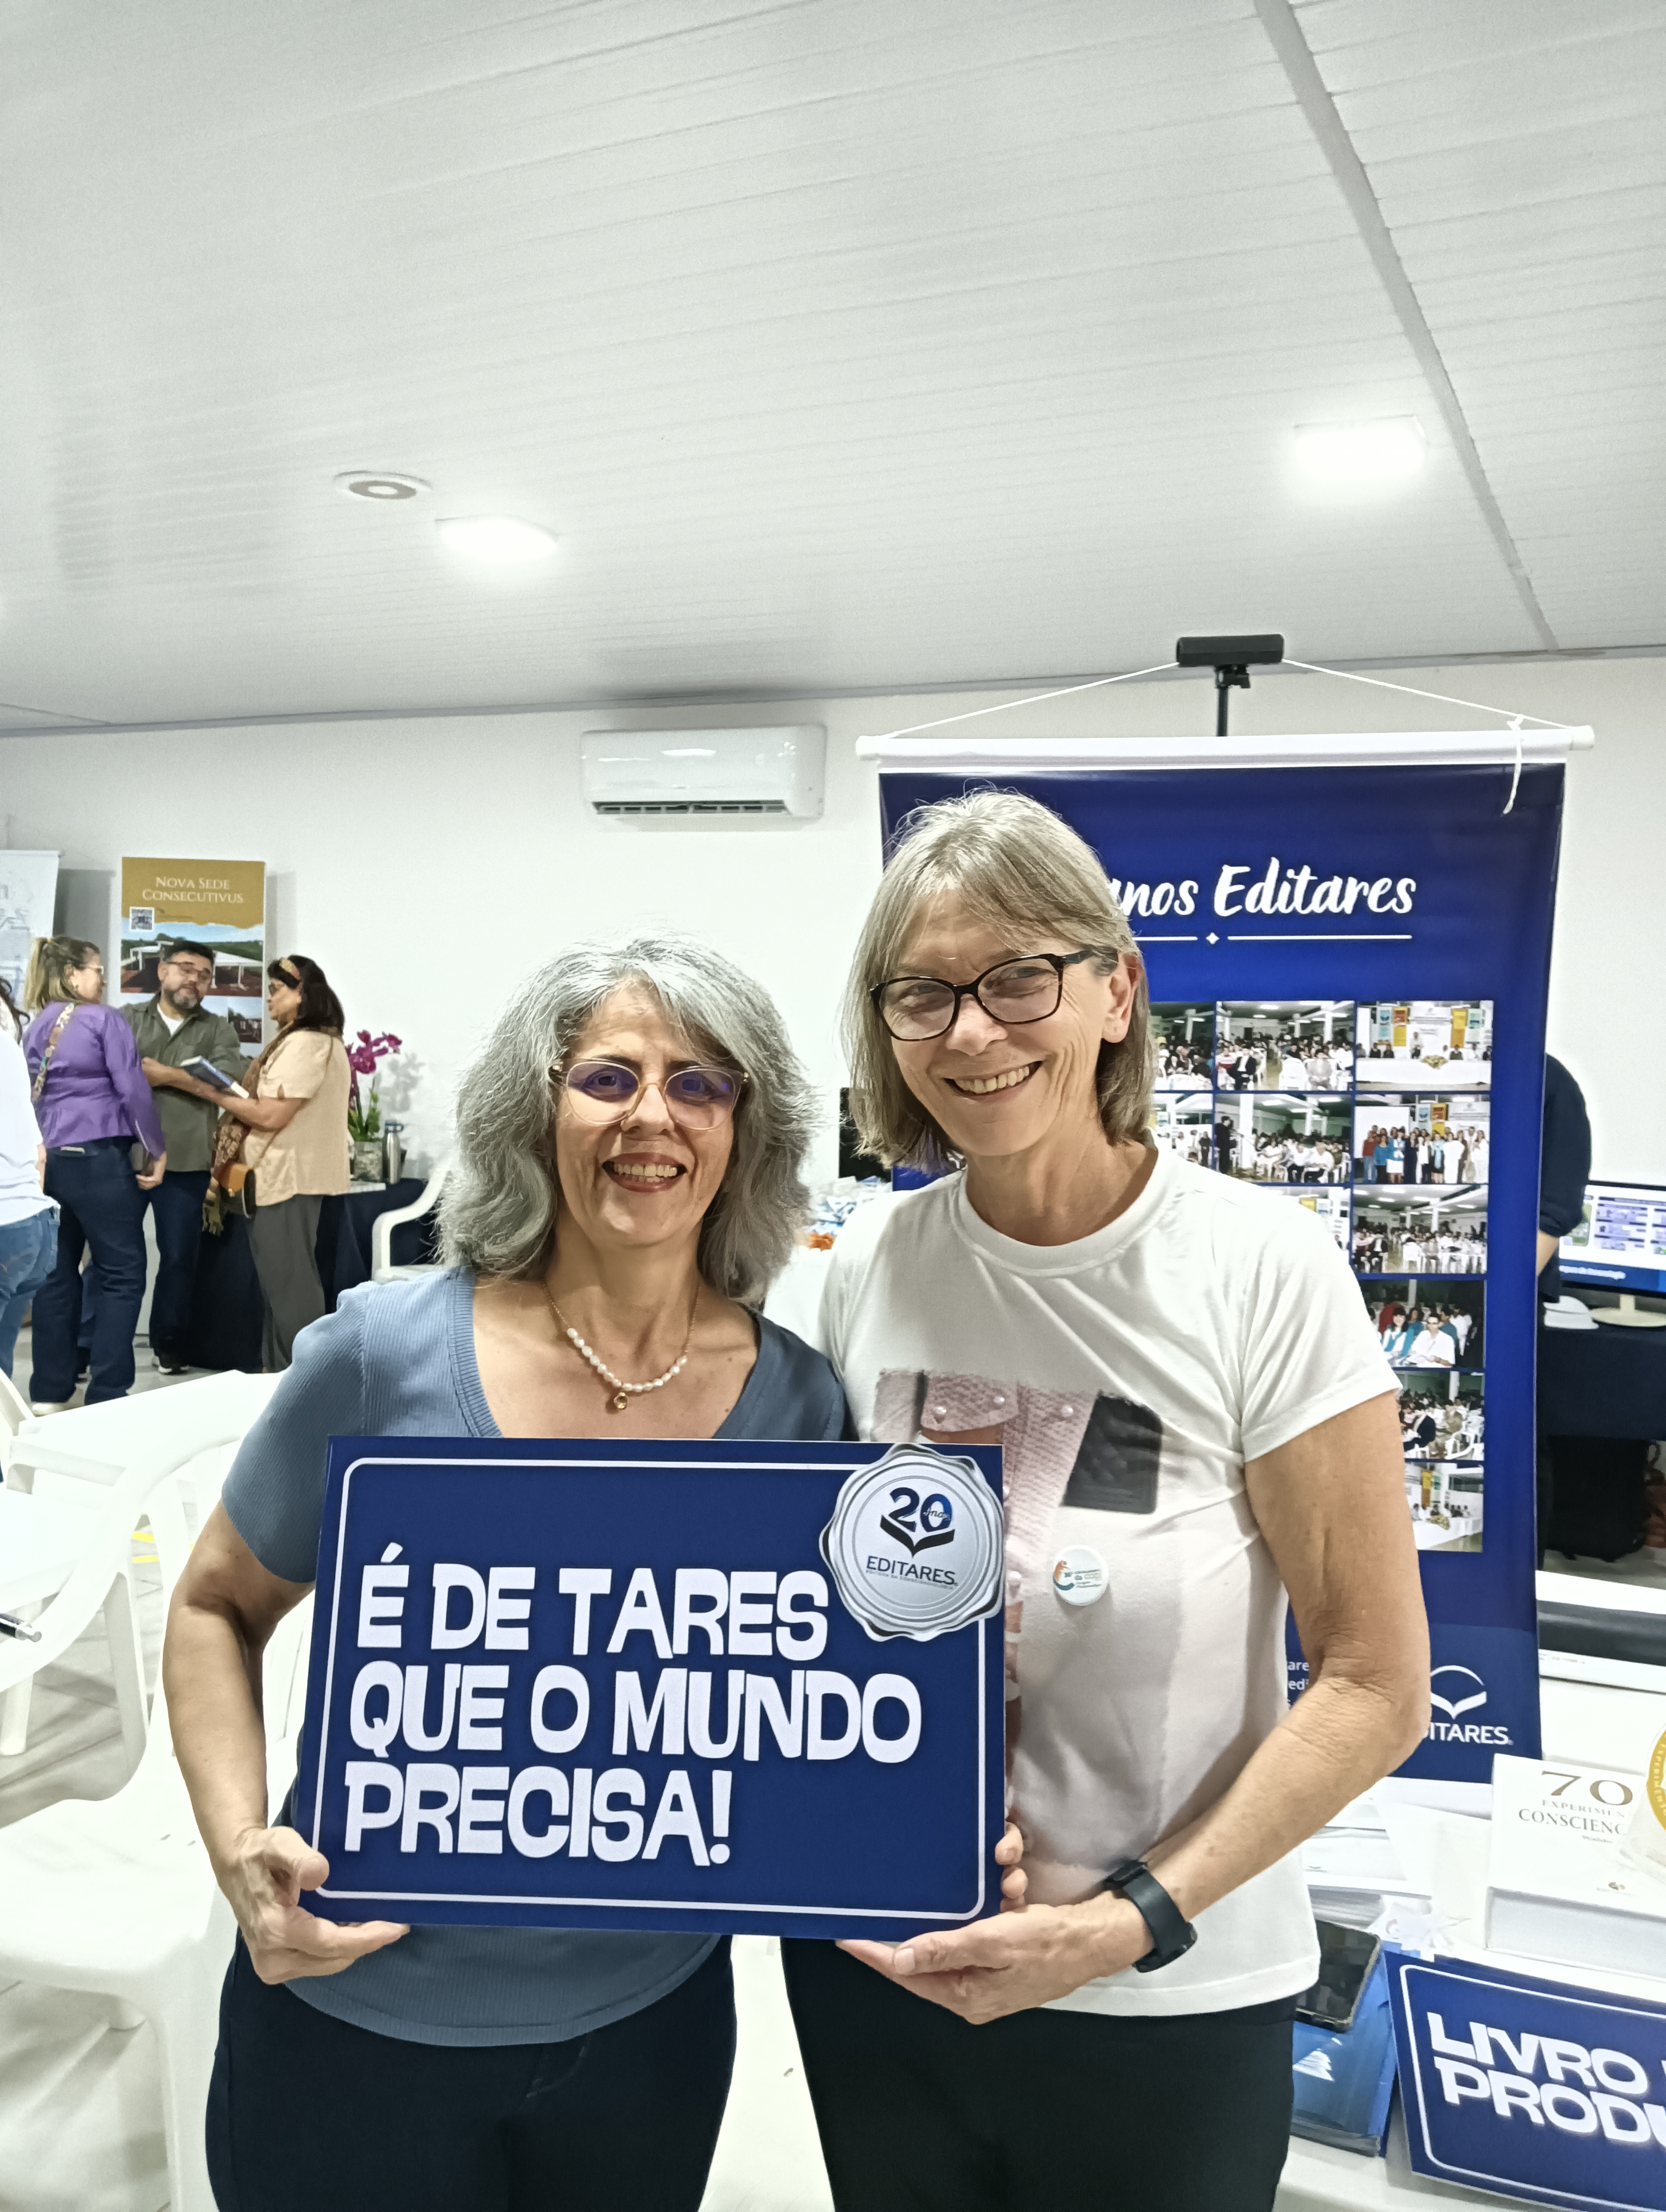
\includegraphics[width=8cm,trim={100 0 100 1100},clip]{articles/resumo/fotos/materia2/IMG20241208144410.jpg}
    \end{center}



\textbf{Como foi o convite ou o processo de chegada de vocês à coordenação da Editares? Quais eram suas expectativas ao assumir e como elas se confirmaram ou mudaram nesses dois anos?}

\textbf{Ana:} Foi um convite bastante refletido. Precisei pensar muito antes de aceitar, porque já tinha diversas atividades. Houve um grande investimento da liderança da Editares para que eu assumisse a coordenação, e uma condição era ter coordenação em dupla. Então, Cristina Ellwanger convidou a Magda.

\textbf{Magda:} Eu já tinha decidido que só toparia se fosse com a Ana. Se ela aceitasse, eu ficaria junto.

\textbf{Ana:} No início, eu não tinha muitas expectativas. As ideias foram surgindo com o tempo e fomos fazendo acontecer. Começamos organizando os contratos de cessão de direitos e planejando a mudança da sala, para acomodar melhor a equipe e atender os autores e neo-autores.

\textbf{Magda:} Eu tinha feito o curso de preparação de lideranças da Unicin, mas na época não compreendia bem o que representava. No curso, cheguei a dizer que não assumiria nenhuma gestão. Perguntaram do que eu estava me escondendo --- e essa pergunta ficou ecoando, me fazendo refletir.

\textbf{Ana:} Eu também não pensava em coordenação, nem em voluntariar na Editares. Mas, ao publicar o livro Antologia da Técnica de Mais 1 Ano de Vida Intrafísica, juntamente com mais 3 organizadoras, senti vontade de ajudar mais, pois me identifiquei com o trabalho. Aos poucos, percebi o quanto isso se conectava com a minha proéxis: auxiliar outras pessoas a escreverem seus livros.

\begin{pullquote}
``Aos poucos, percebi o quanto isso se conecta com a minha proéxis: auxiliar outras pessoas a escreverem seus livros.''
\end{pullquote}

\textbf{Quais foram os maiores desafios enfrentados na gestão da editora nesse período? Que aprendizados pessoais e grupais vocês destacariam dessa experiência?}

\textbf{Ana:} Um dos maiores desafios foi formar equipes e reestruturar o Conselho Editorial e o fluxo editorial. Outro, foi dar mais celeridade às publicações preservando a qualidade. Isso só foi possível graças ao envolvimento dos voluntários, autores, editores e de voluntários da CCCI. Mostramos do que somos capazes quando trabalhamos juntos. Conseguimos organizar o fluxo de chegada das obras, fazer o acompanhamento até a publicação e manter um bom ritmo. Essa “máquina” só funciona porque contamos com especialistas para revisão, conferência e apoio editorial. Hoje, tudo flui bem em razão do esforço coletivo.

\textbf{Magda:} Essa experiência exigiu um amadurecimento na gestão, porque tivemos que desenvolver uma visão de conjunto. Para mim, um desafio marcante foi a perda das informações  do sistema de gestão de vendas dos livros. Perdemos dados atualizados e tivemos que fazer um esforço enorme para recuperá-los. Trabalhei lado a lado com a Angélica {[funcionária da Editares]} nessa fase. A Ana estava viajando, e isso acabou ajudando, porque ela conseguia me acalmar e me manter focada na solução. Essa parceria na coordenação funcionou muito bem: quando uma estava sobrecarregada, a outra dava suporte.

\textbf{Que efeitos essa experiência trouxe para a autopesquisa e a proéxis de cada uma?}

\textbf{Ana:} Para mim, foi como se eu tivesse me localizado na proéxis. É como se tivesse feito um ``download'' não só da intermissão, mas também de experiências de outras vidas. Estar na linha de frente, na ``vitrine'', não era algo natural para mim. Aprendi a lidar com a exposição, a assumir responsabilidades com mais maturidade e a mostrar quem eu realmente sou --- com meus traf\emph{o}res, traf\emph{a}res e traf\emph{ai}s. Um dos maiores aprendizados foi não limitar meus potenciais por medo de errar ou aparecer. A vivência me ajudou a superar essas barreiras internas.

\textbf{Magda:} Para mim, a gestão ampliou muito minha visão. Passei a enxergar melhor o funcionamento do grupo, amadureci e desenvolvi um senso maior de pertencimento à Comunidade Conscienciológica. Essa sensação de estar integrada e contribuir para algo maior é muito gratificante.

\textbf{Como vocês imaginam o futuro da editoração conscienciológica?}

\textbf{Ana:} Gostaria que conseguíssemos dar ainda mais celeridade às publicações. Para isso, precisamos que as obras cheguem mais bem estruturadas, o que permitiria avançar com mais rapidez sem perder a qualidade. Estamos trabalhando nesse sentido.

\textbf{Magda:} A parceria com a Uniescon pode contribuir bastante nesse processo.

\textbf{Ana:} Além disso, seria importante ampliar o engajamento de voluntários da CCCI, especialmente aqueles com disponibilidade para atuar nas revisões.

\textbf{Que mensagem final gostariam de deixar para os leitores e voluntários da Conscienciologia?}

\textbf{Ana:} Se uma oportunidade ou desafio bater à sua porta, abrace-o e leve até o fim. No final, reflita: \emph{o que aprendi com isso?}

\begin{pullquote}
``Se uma oportunidade ou desafio bater à sua porta, abrace-o e leve até o fim. No final, reflita: \emph{o que aprendi com isso?}''
\end{pullquote}

\textbf{Magda:} Apesar dos desafios da coordenação, esse trabalho vale muito a pena. Ele contribui diretamente para o amadurecimento pessoal, grupal e intraconsciencial.

\coverart{../fundo-generico.png}

\textbf{Coordenadoras:} Agradecemos a todos os voluntários da Editares e da CCCI que contribuem e fazem parte desse trabalho interassistencial de publicação de obras conscienciológicas, ajudando a materializar as proéxis individuais e a maxiproéxis grupal!

%    \begin{center}
%        %  trim={<left> <lower> <right> <upper>}
%        
\includegraphics[width=8.5cm,trim={0 740 0 50},clip]{articles/resumo/fotos/editares-20anos.jpg}
%    \end{center}



%\begin{pullquote}
%``Aos poucos, percebi o quanto isso se conecta com a minha proéxis: auxiliar outras pessoas a escreverem seus livros.''
%\end{pullquote}

        
    \end{multicols}



% \begin{center}
%     \noindent\includegraphics[width=14cm, height=10cm]{example-image}
% \end{center}

\end{document}

    \documentclass{gescons}

\genre {Resumo do Biênio}
\author{Amanda Vieira}
\title{Editares Celebra 20 Anos com Programação Especial}

\begin{document}
    \makeentrevistatitle
    %\maketitle

    %\fullwidthimage{fields}{b}

    %\coverart{back/editorial}
    \coverart{../fundo-generico.png}
    
    \begin{multicols}{2}

%\begin{center}
%    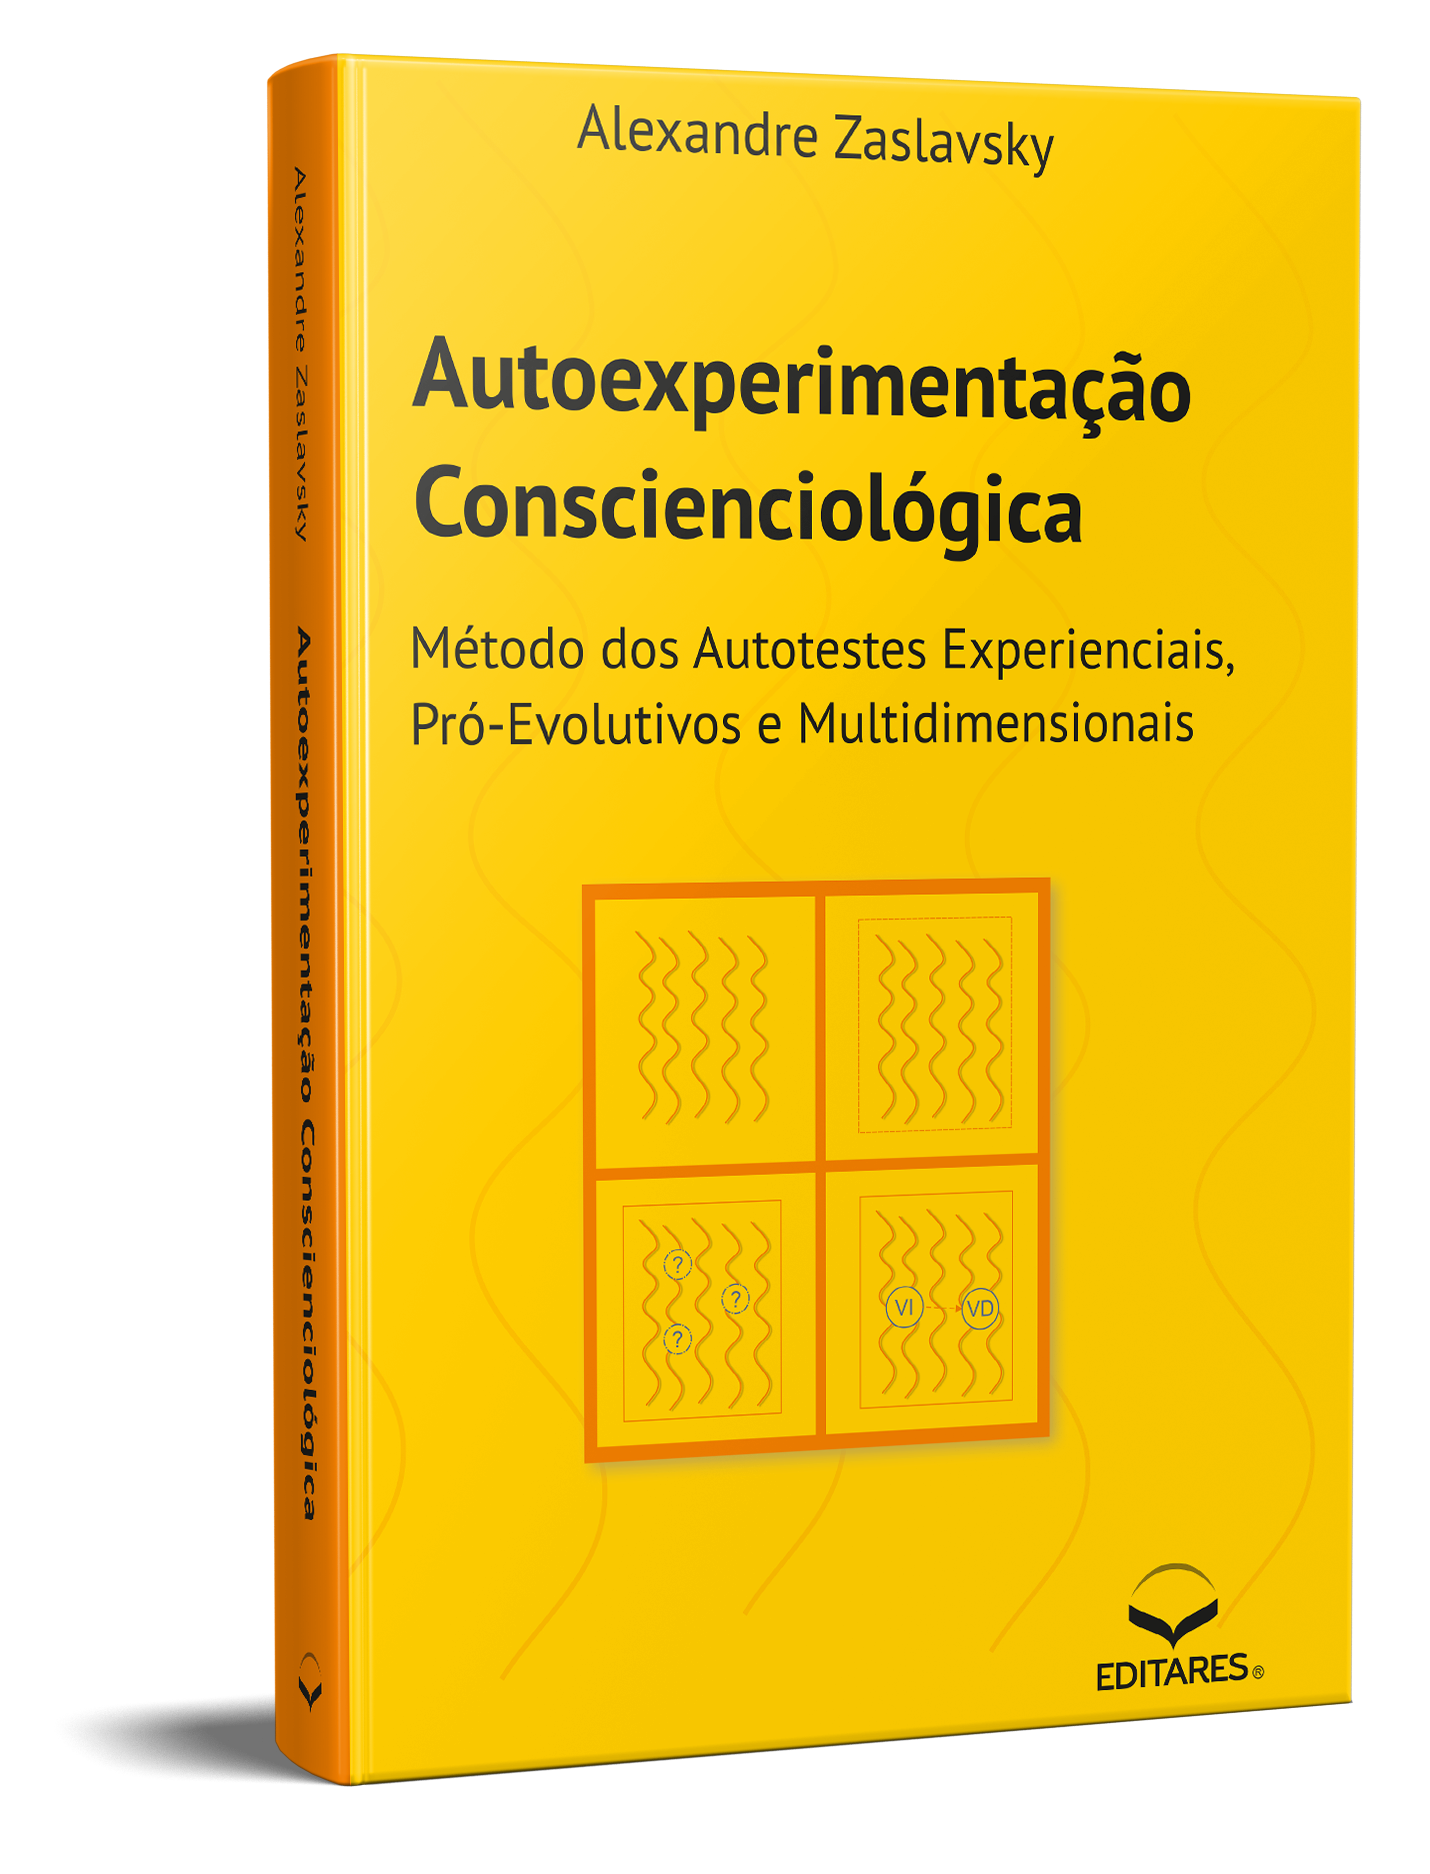
\includegraphics[width=4cm]{articles/entrevista/mockups/Alexandre-Zas.png}
%\end{center}

\textbf{}

\noindent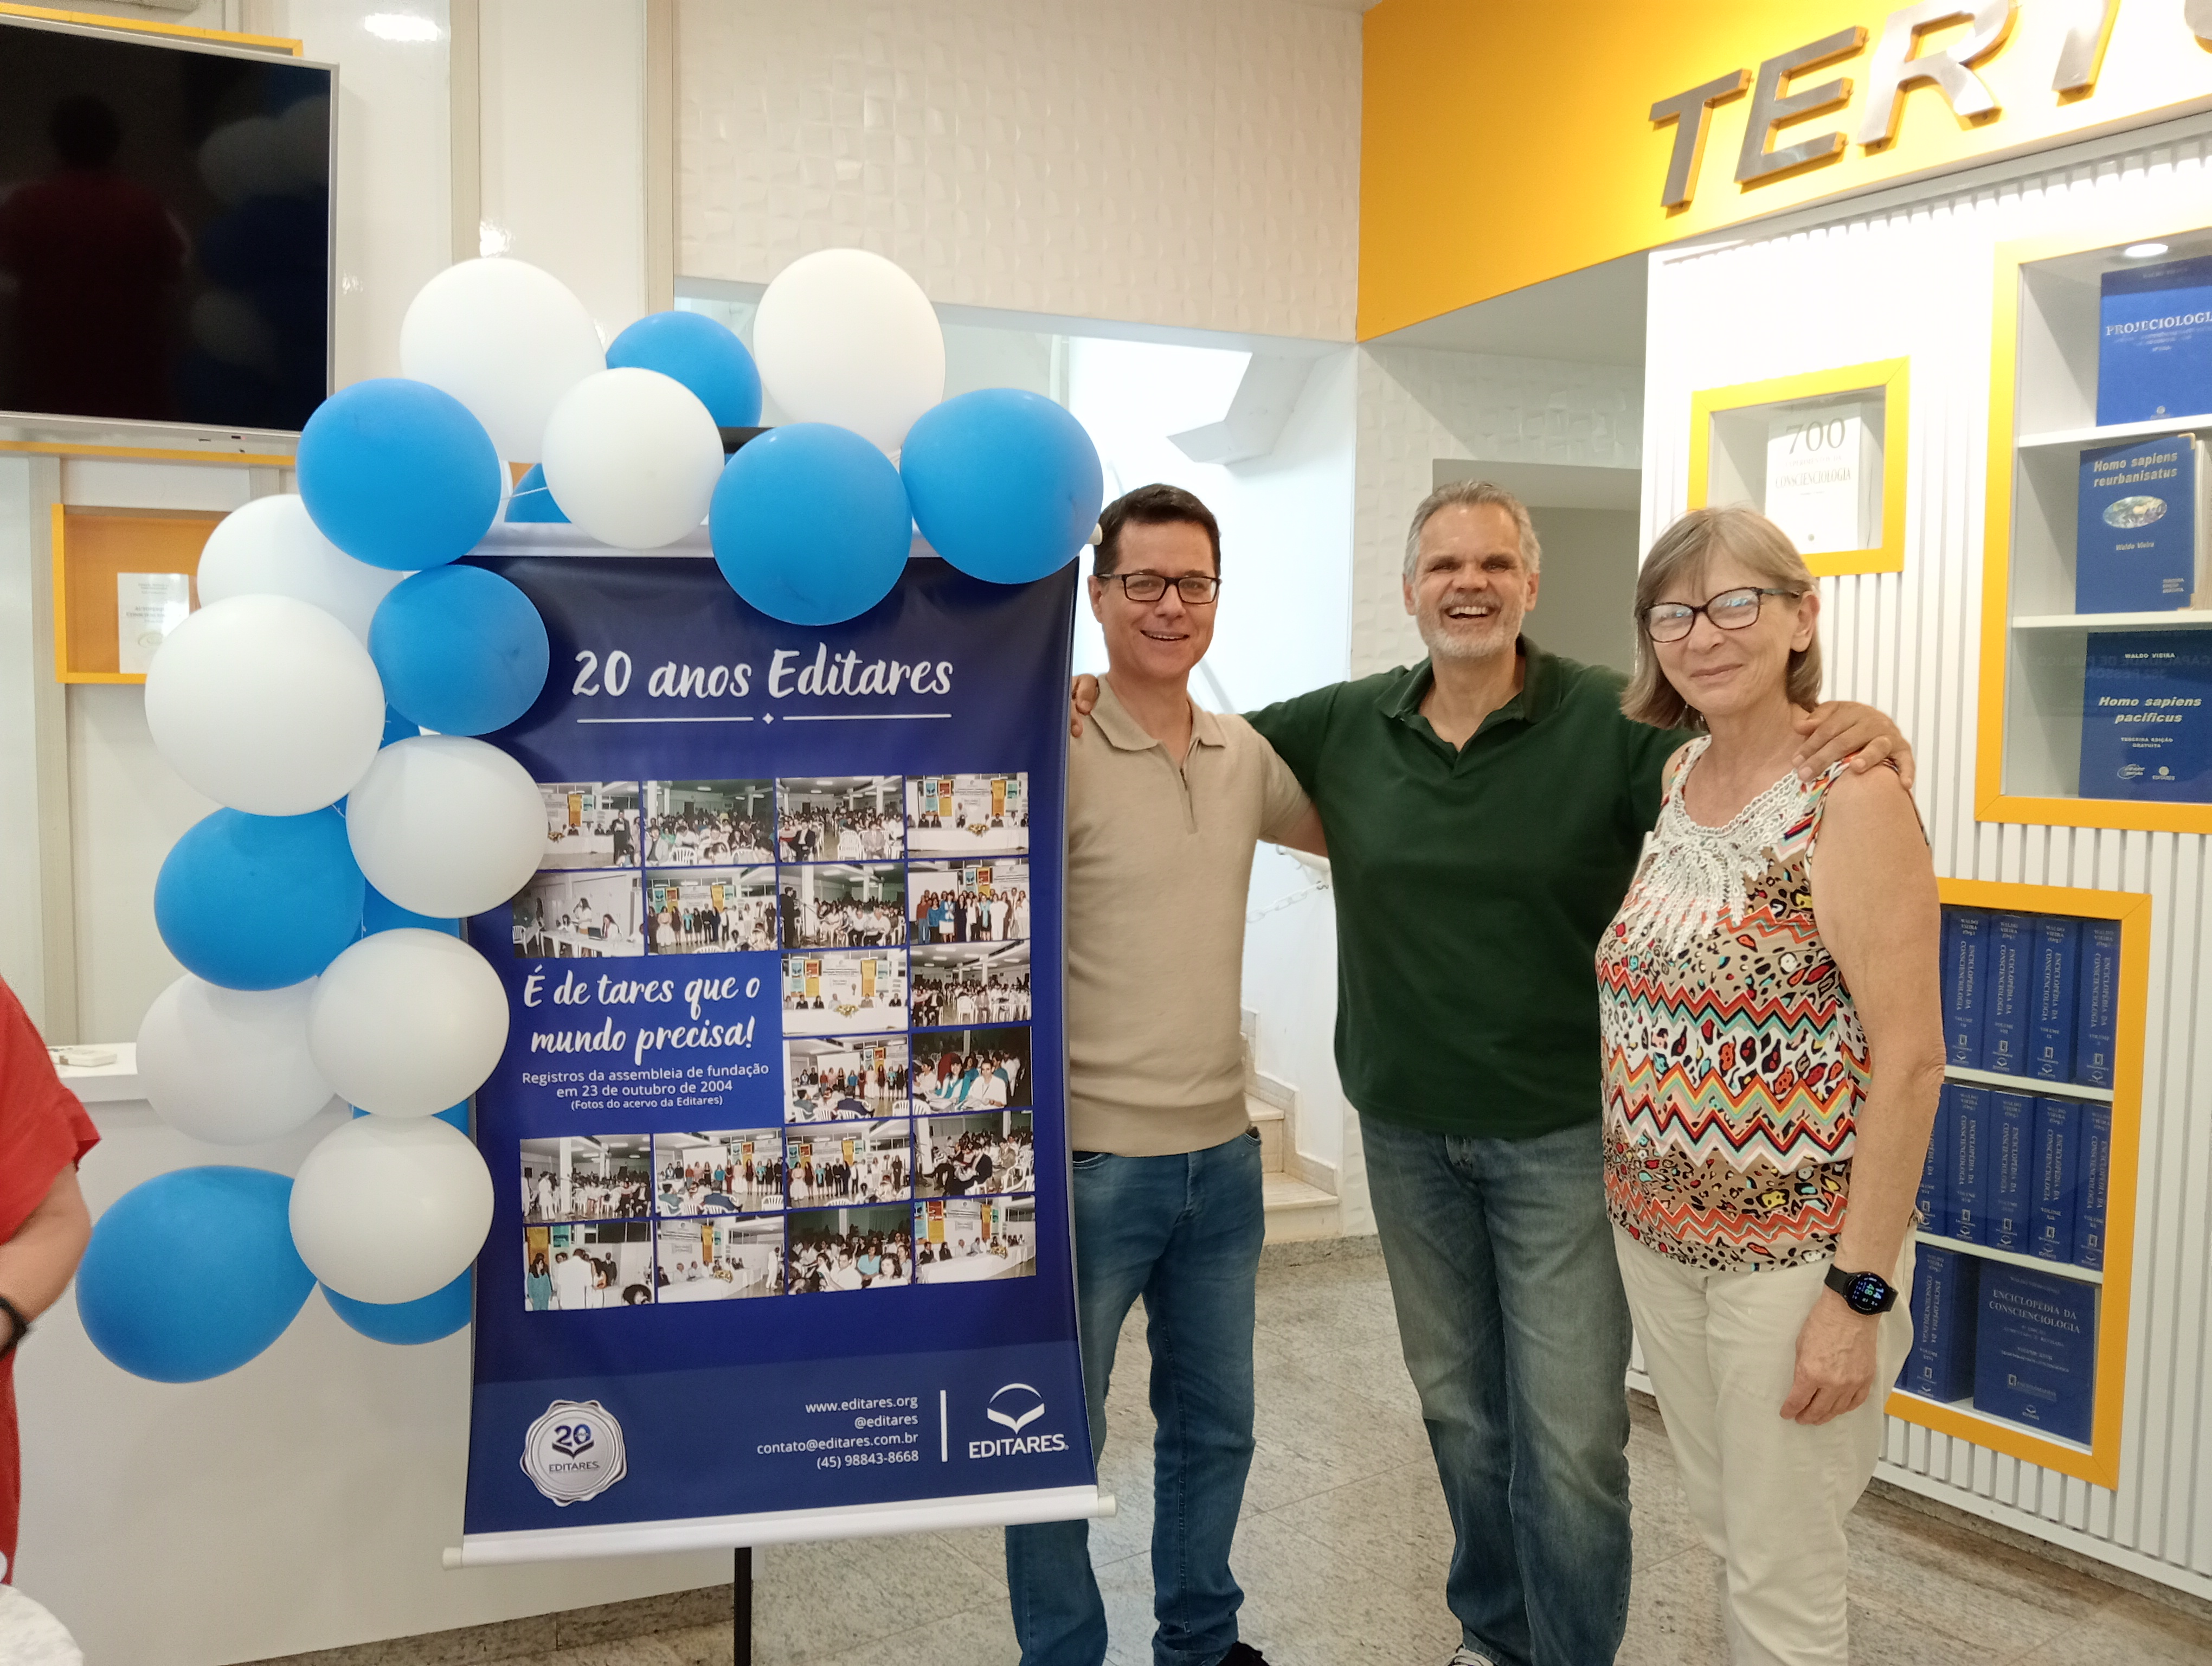
\includegraphics[width=9cm]{articles/resumo/fotos/materia1/IMG20241023144802.jpg}


No dia 23 de outubro de 2024, a~Editares completou duas décadas de atuação dedicada à~publicação técnico-científica de obras conscienciológicas. Para marcar os 20 anos de existência, a~editora promoveu uma série de atividades comemorativas ao longo da semana, integrando voluntários, autores e~leitores em momentos de reflexão, confraternização e~interassistência.

A programação contou com uma \textbf{semana de verbetes temáticos,} realizada no \emph{Tertuliarium} do CEAEC, com a~participação de autores e~leitores em debates e~apresentações de temas relacionados ao propósito editorial da Editares. Também houve um \textbf{Círculo Mentalsomático temático,} focado na escrita interassistencial e~na importância das publicações para a~expansão da Conscienciologia.

Um dos pontos altos da celebração foi o~\textbf{lançamento do livro ``Interassistência'',} de autoria da voluntária do Conselho Editorial, \textbf{Roberta Bouchardet.} A~obra amplia a~abordagem da assistência multidimensional.

Além das atividades de debate, os voluntários participaram de um \textbf{jantar temático português,} organizado pelo restaurante Primener, no campus do CEAEC. A~noite foi marcada pelo clima de gratidão e~união entre os voluntários da Editares e~convidados.

No dia 23, data oficial do aniversário, a~comemoração seguiu após a~Tertúlia, com \textbf{bolo comemorativo e~momentos de confraternização} entre voluntários, amigos e~apoiadores da Editares, celebrando o~continuísmo do trabalho em equipe e~o~compromisso com a~tarefa esclarecedora.

Com 20 anos de história, a~Editares reafirma seu papel na difusão da Conscienciologia por meio da escrita e~da publicação de obras que promovem o~esclarecimento e~a~evolução das consciências. A~celebração reforçou o~valor da escrita interassistencial ao modo de instrumento de mudança e~continuidade da maxiproéxis grupal.

% {[}COLOCAR ALGUMAS FOTOS{]} As fotos estão na pasta do drive: Matéria 1: Editares celebra 20 anos com programação especial - elas podem ser num tamanho pequeno; aparecer no final ou intercalando com o~texto

%\begin{pullquote}
%``A escrita de uma obra conscienciológica é~uma oportunidade evolutiva inigualável.''
%\end{pullquote}

\noindent
\includegraphics[width=9cm]{articles/resumo/fotos/materia1/IMG20241023143149.jpg}
        
    \end{multicols}
\end{document}

    \documentclass{gescons}

\genre {Resumo do Biênio}
\author{Amanda Vieira}
\title{Editares no XXXVI Congraçamento das ICs: Plaquinhas, sorrisos e escrita}

\begin{document}
    \makeentrevistatitle
    %\maketitle

    %\fullwidthimage{fields}{b}

    %\coverart{back/editorial}
    \coverart{../fundo-generico.png}
    
%    \begin{multicols}{2}

%\begin{center}
%    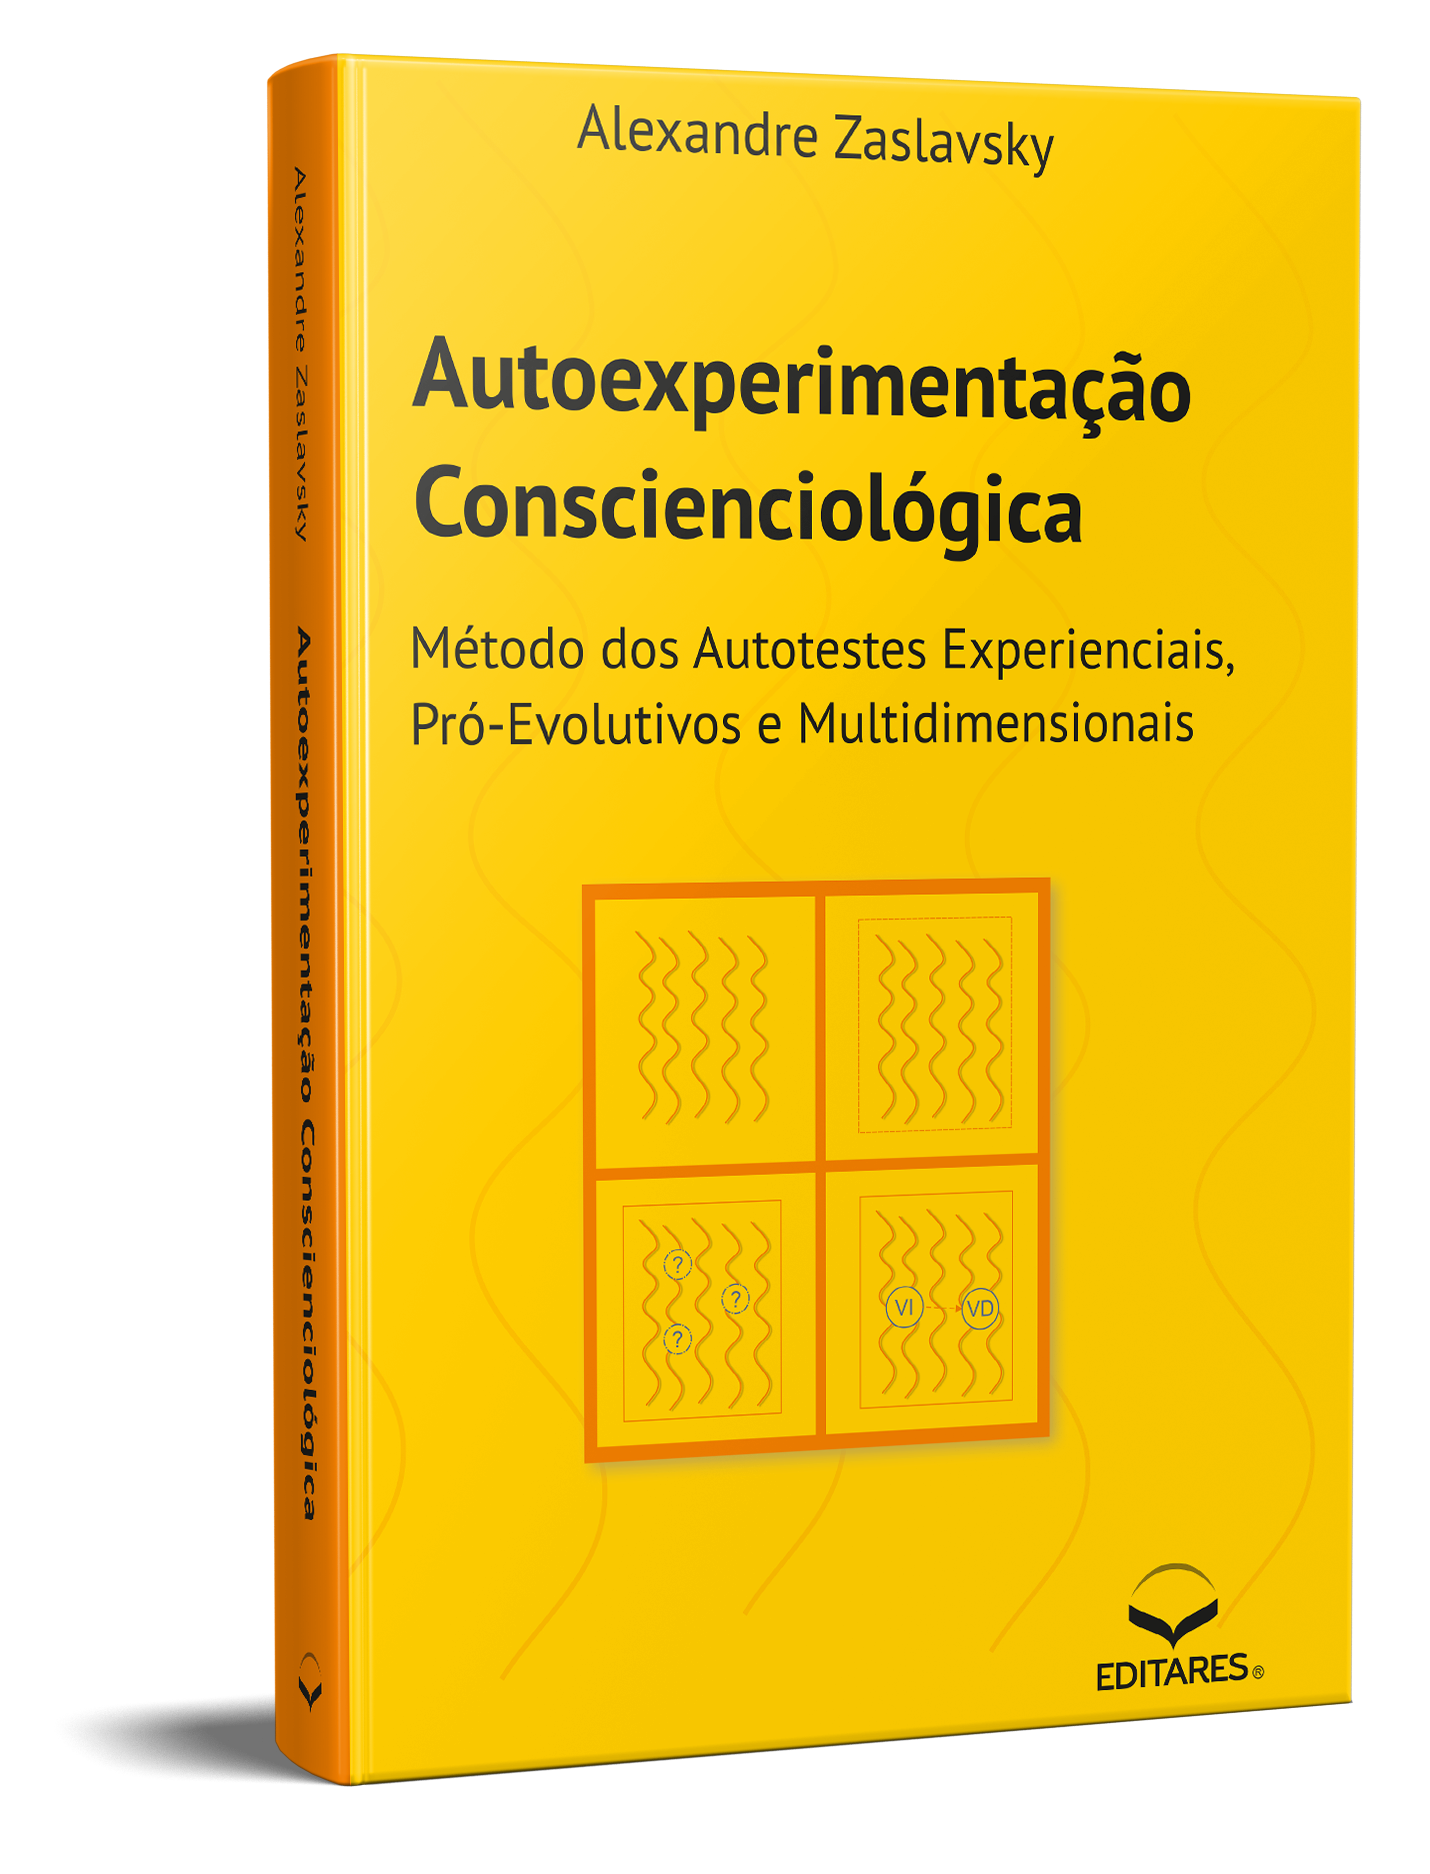
\includegraphics[width=4cm]{articles/entrevista/mockups/Alexandre-Zas.png}
%\end{center}





No dia 8 de dezembro de 2024, durante o tradicional \textbf{Congraçamento das ICs} -- evento anual de celebração do voluntariado conscienciológico --, a Editares marcou presença com uma ação voltada aos \textbf{autores e futuros autores}.

Com placas instigativas e frases de compromisso com a escrita, os voluntários foram convidados a tirar fotos simbolizando o engajamento na tarefa autoral. A atividade trouxe um clima de \textbf{descontração e leveza}, ao mesmo tempo em que reforçou a importância do autoposicionamento proexológico perante a escrita conscienciológica.

\textbf{Confira as fotos!}

  \begin{minipage}[b]{0.32\textwidth}
    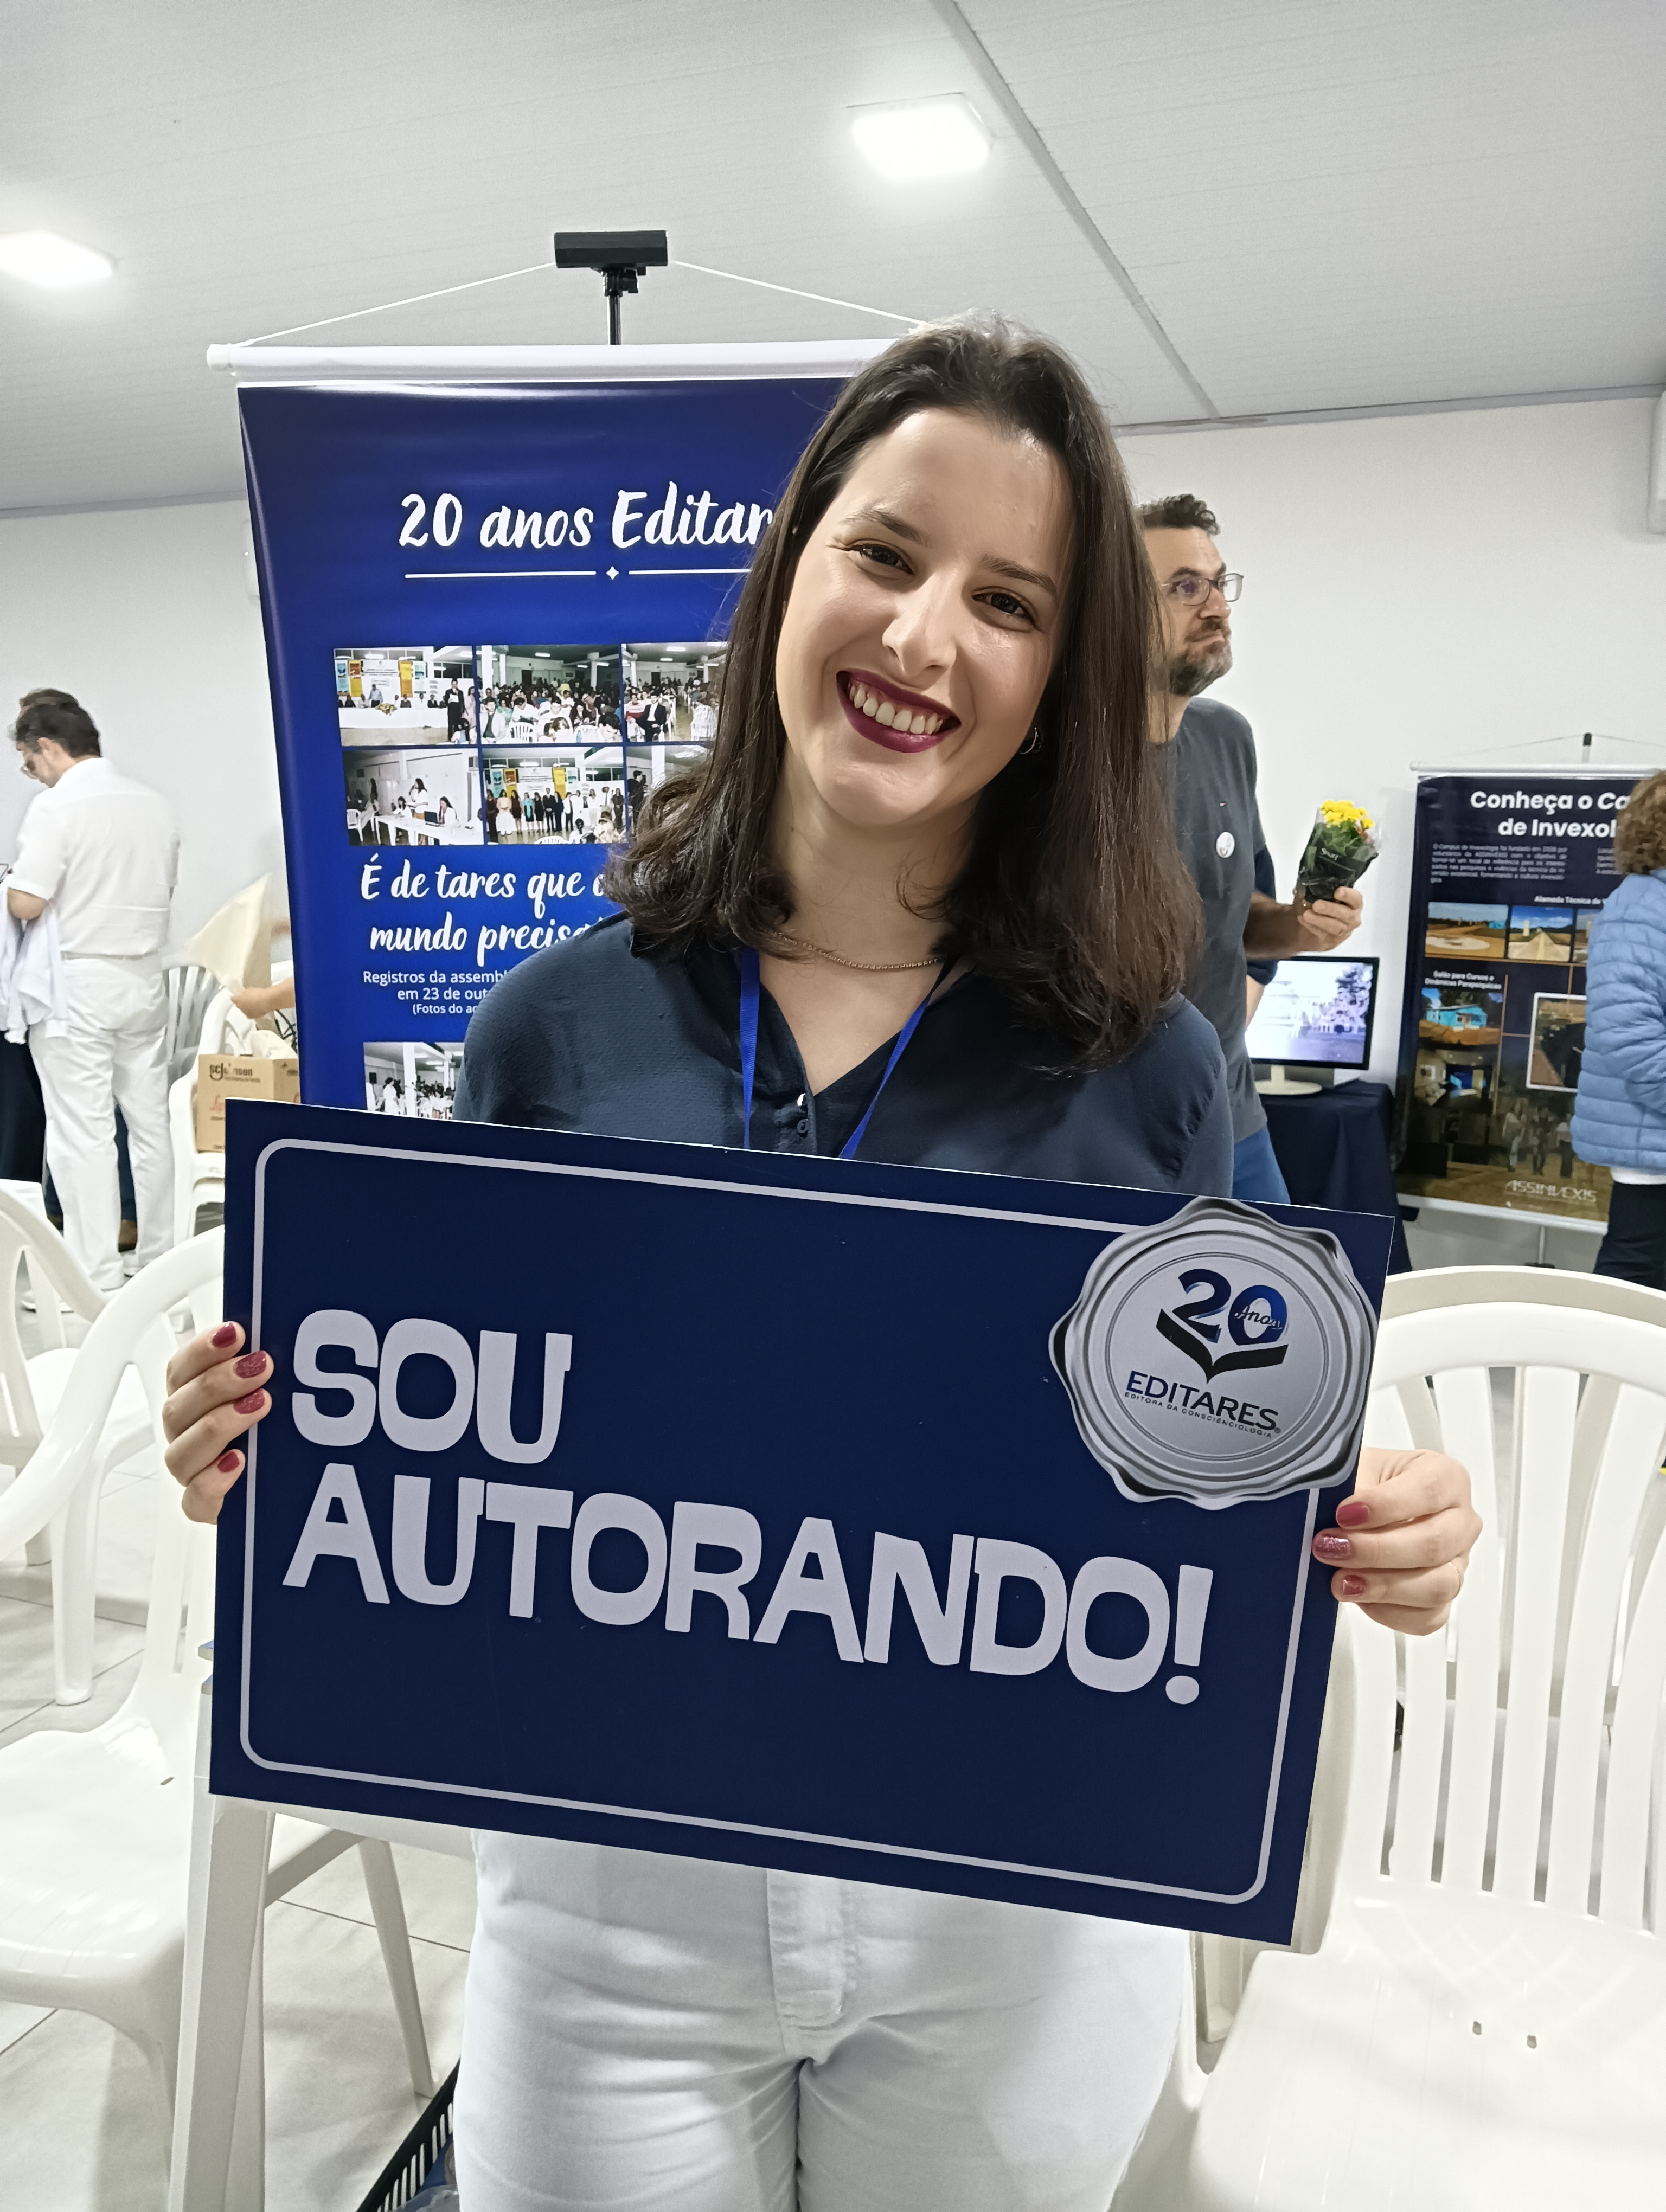
\includegraphics[width=\linewidth]{articles/resumo/fotos/materia2/IMG20241208144202.jpg}
  \end{minipage}\hfill
  \begin{minipage}[b]{0.32\textwidth}
    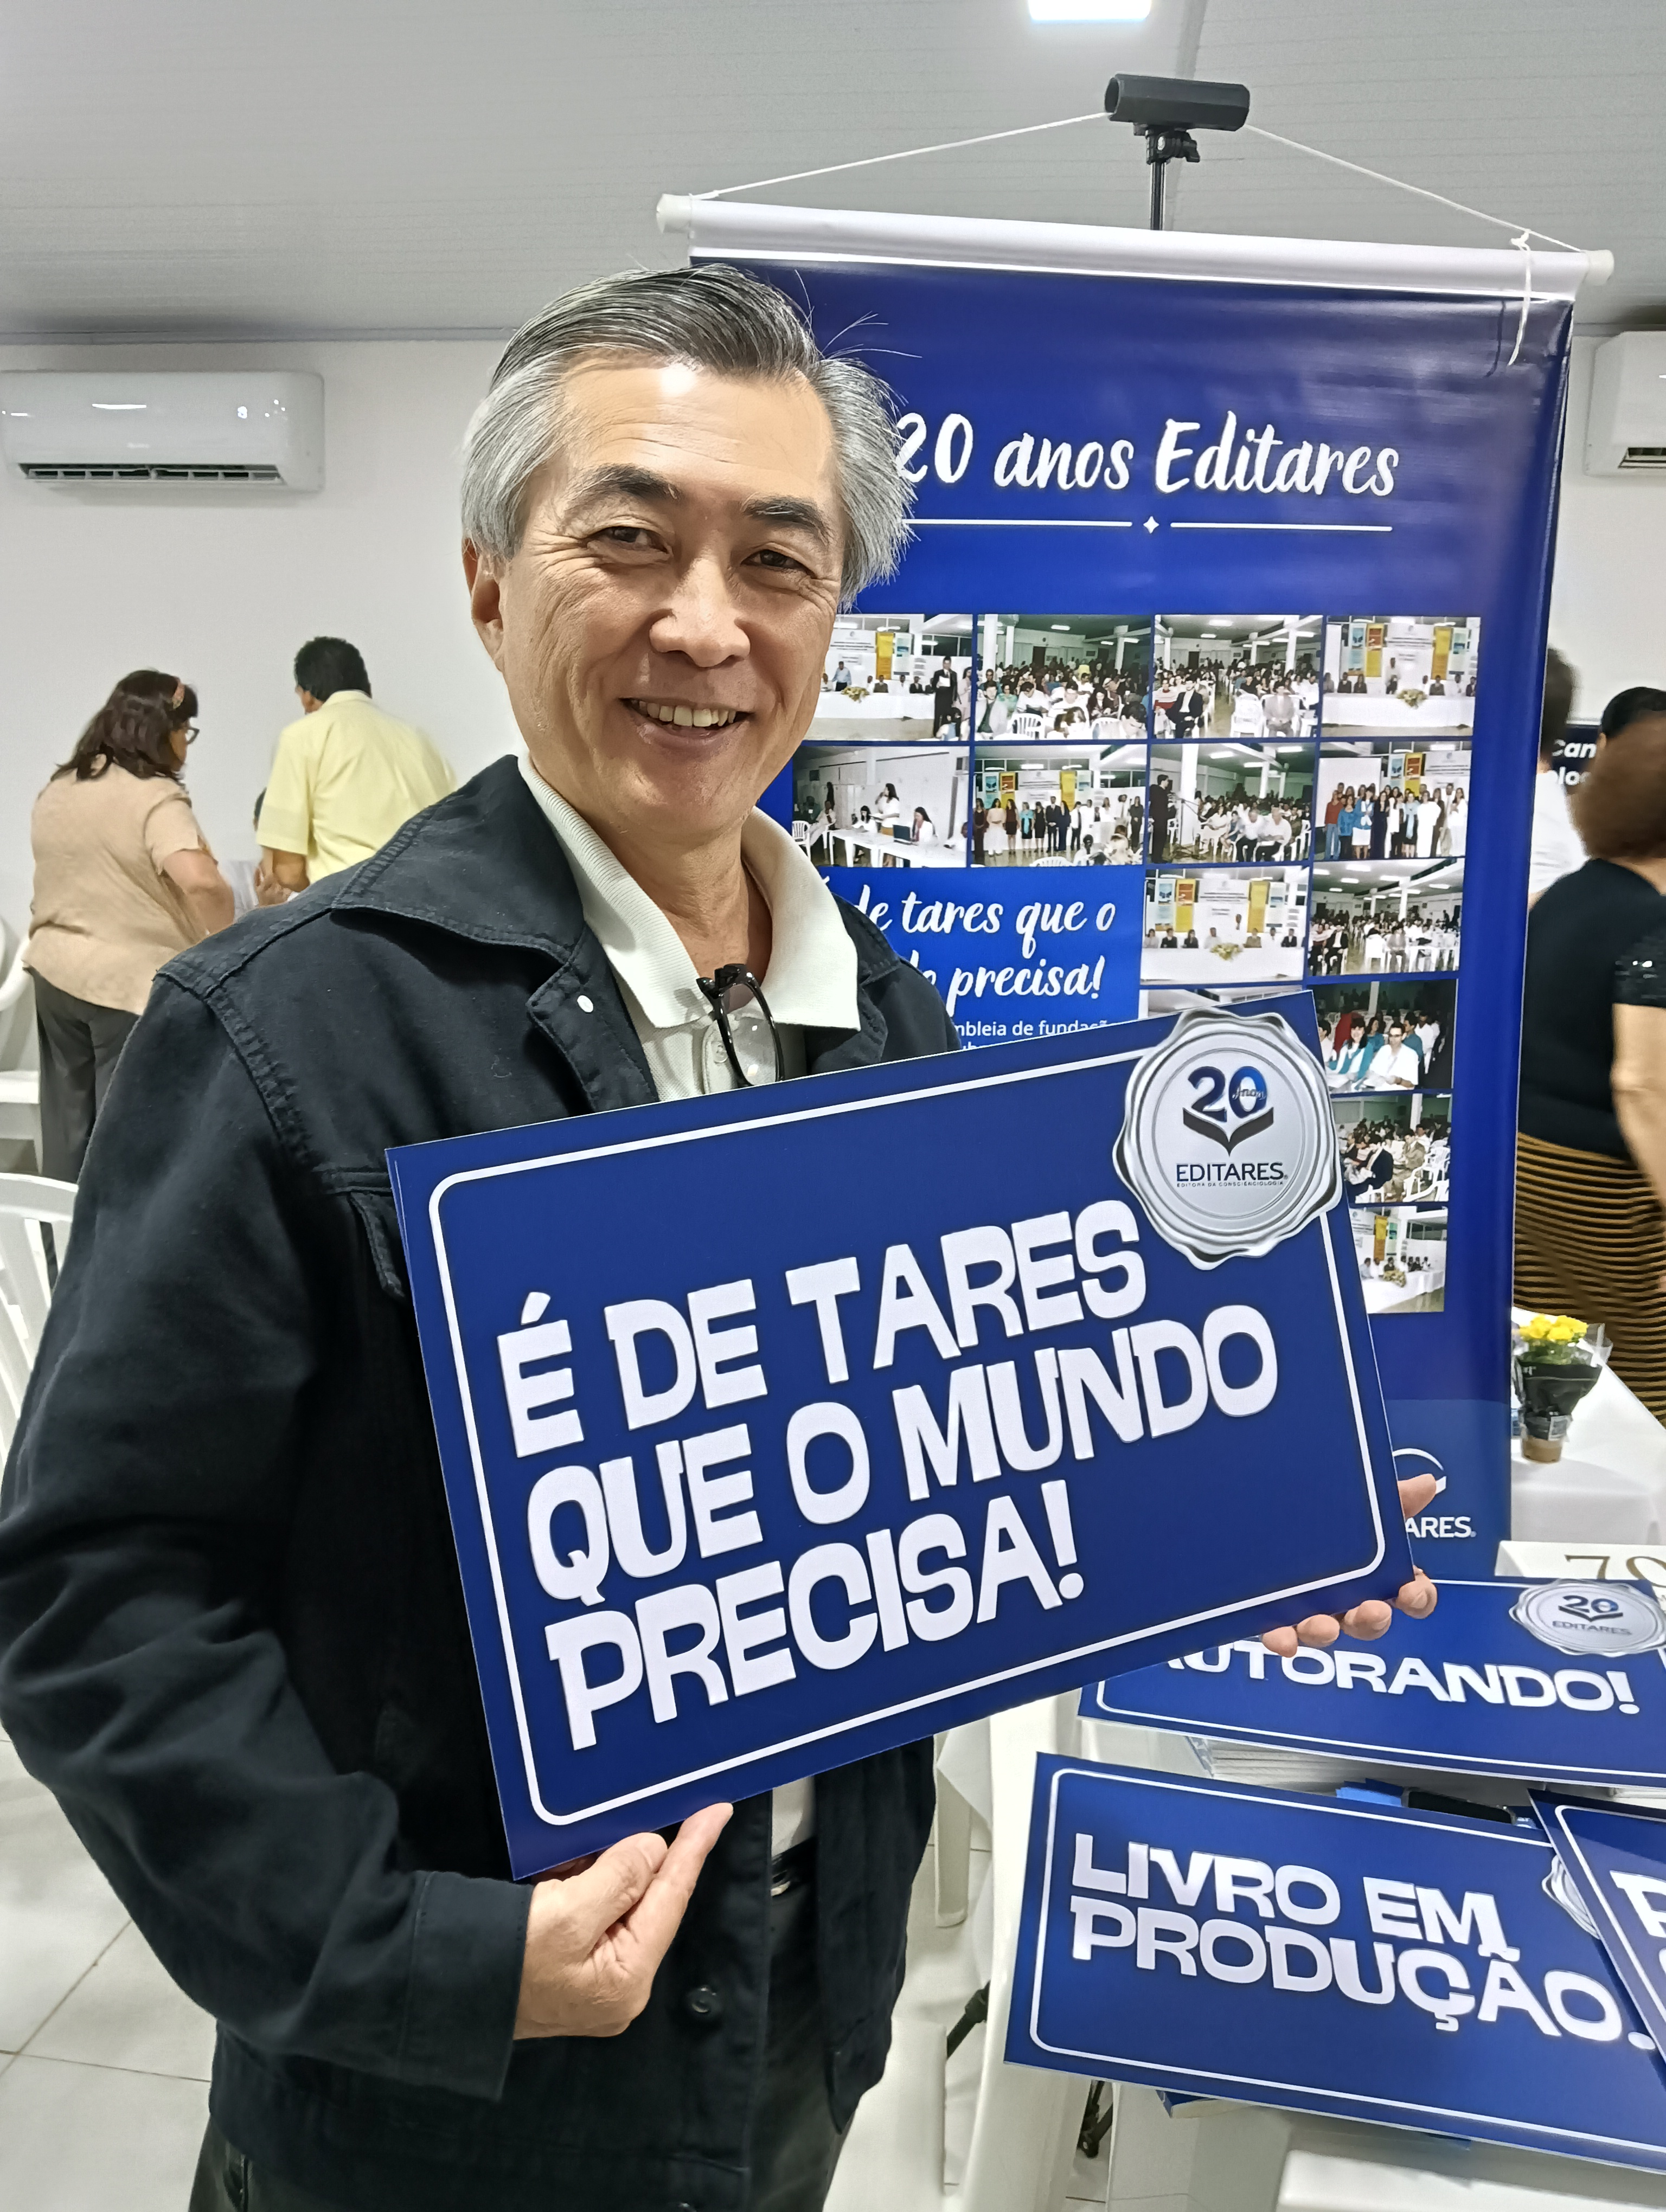
\includegraphics[width=\linewidth]{articles/resumo/fotos/materia2/IMG20241208145756.jpg}
  \end{minipage}\hfill
  \begin{minipage}[b]{0.32\textwidth}
    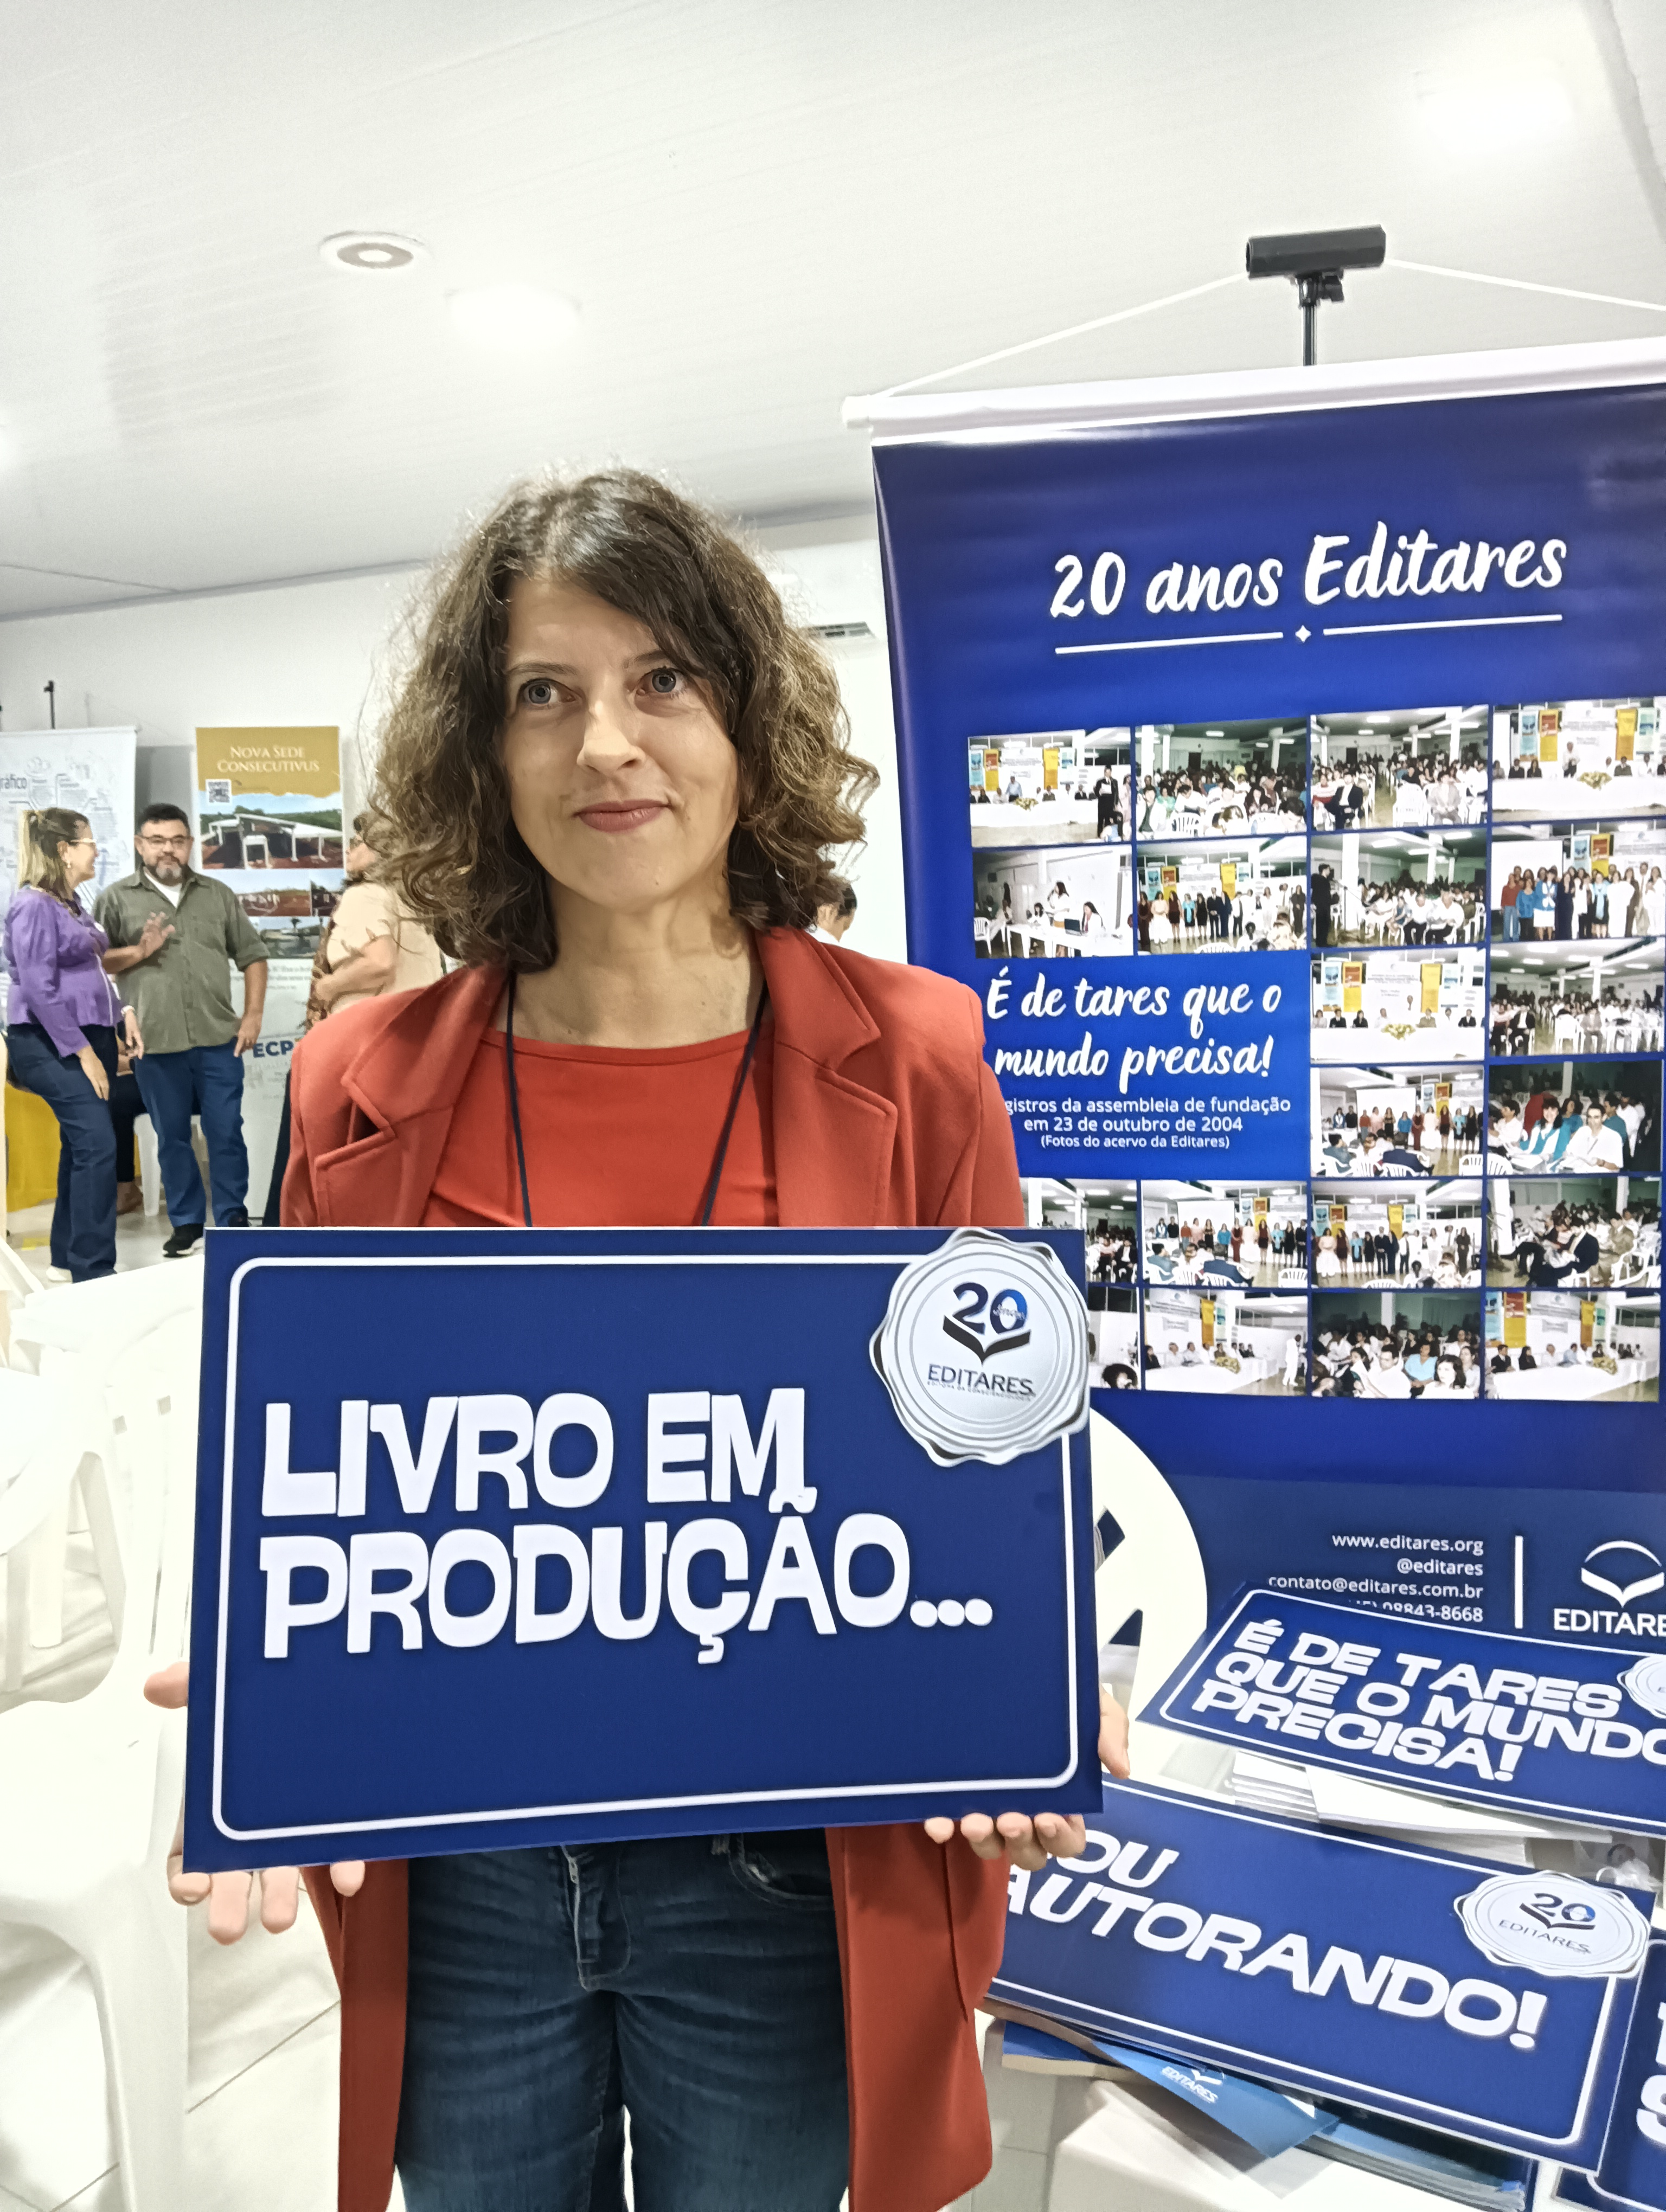
\includegraphics[width=\linewidth]{articles/resumo/fotos/materia2/IMG20241208144514.jpg}
  \end{minipage}
  
  \centering
  \begin{minipage}[b]{0.32\textwidth}
    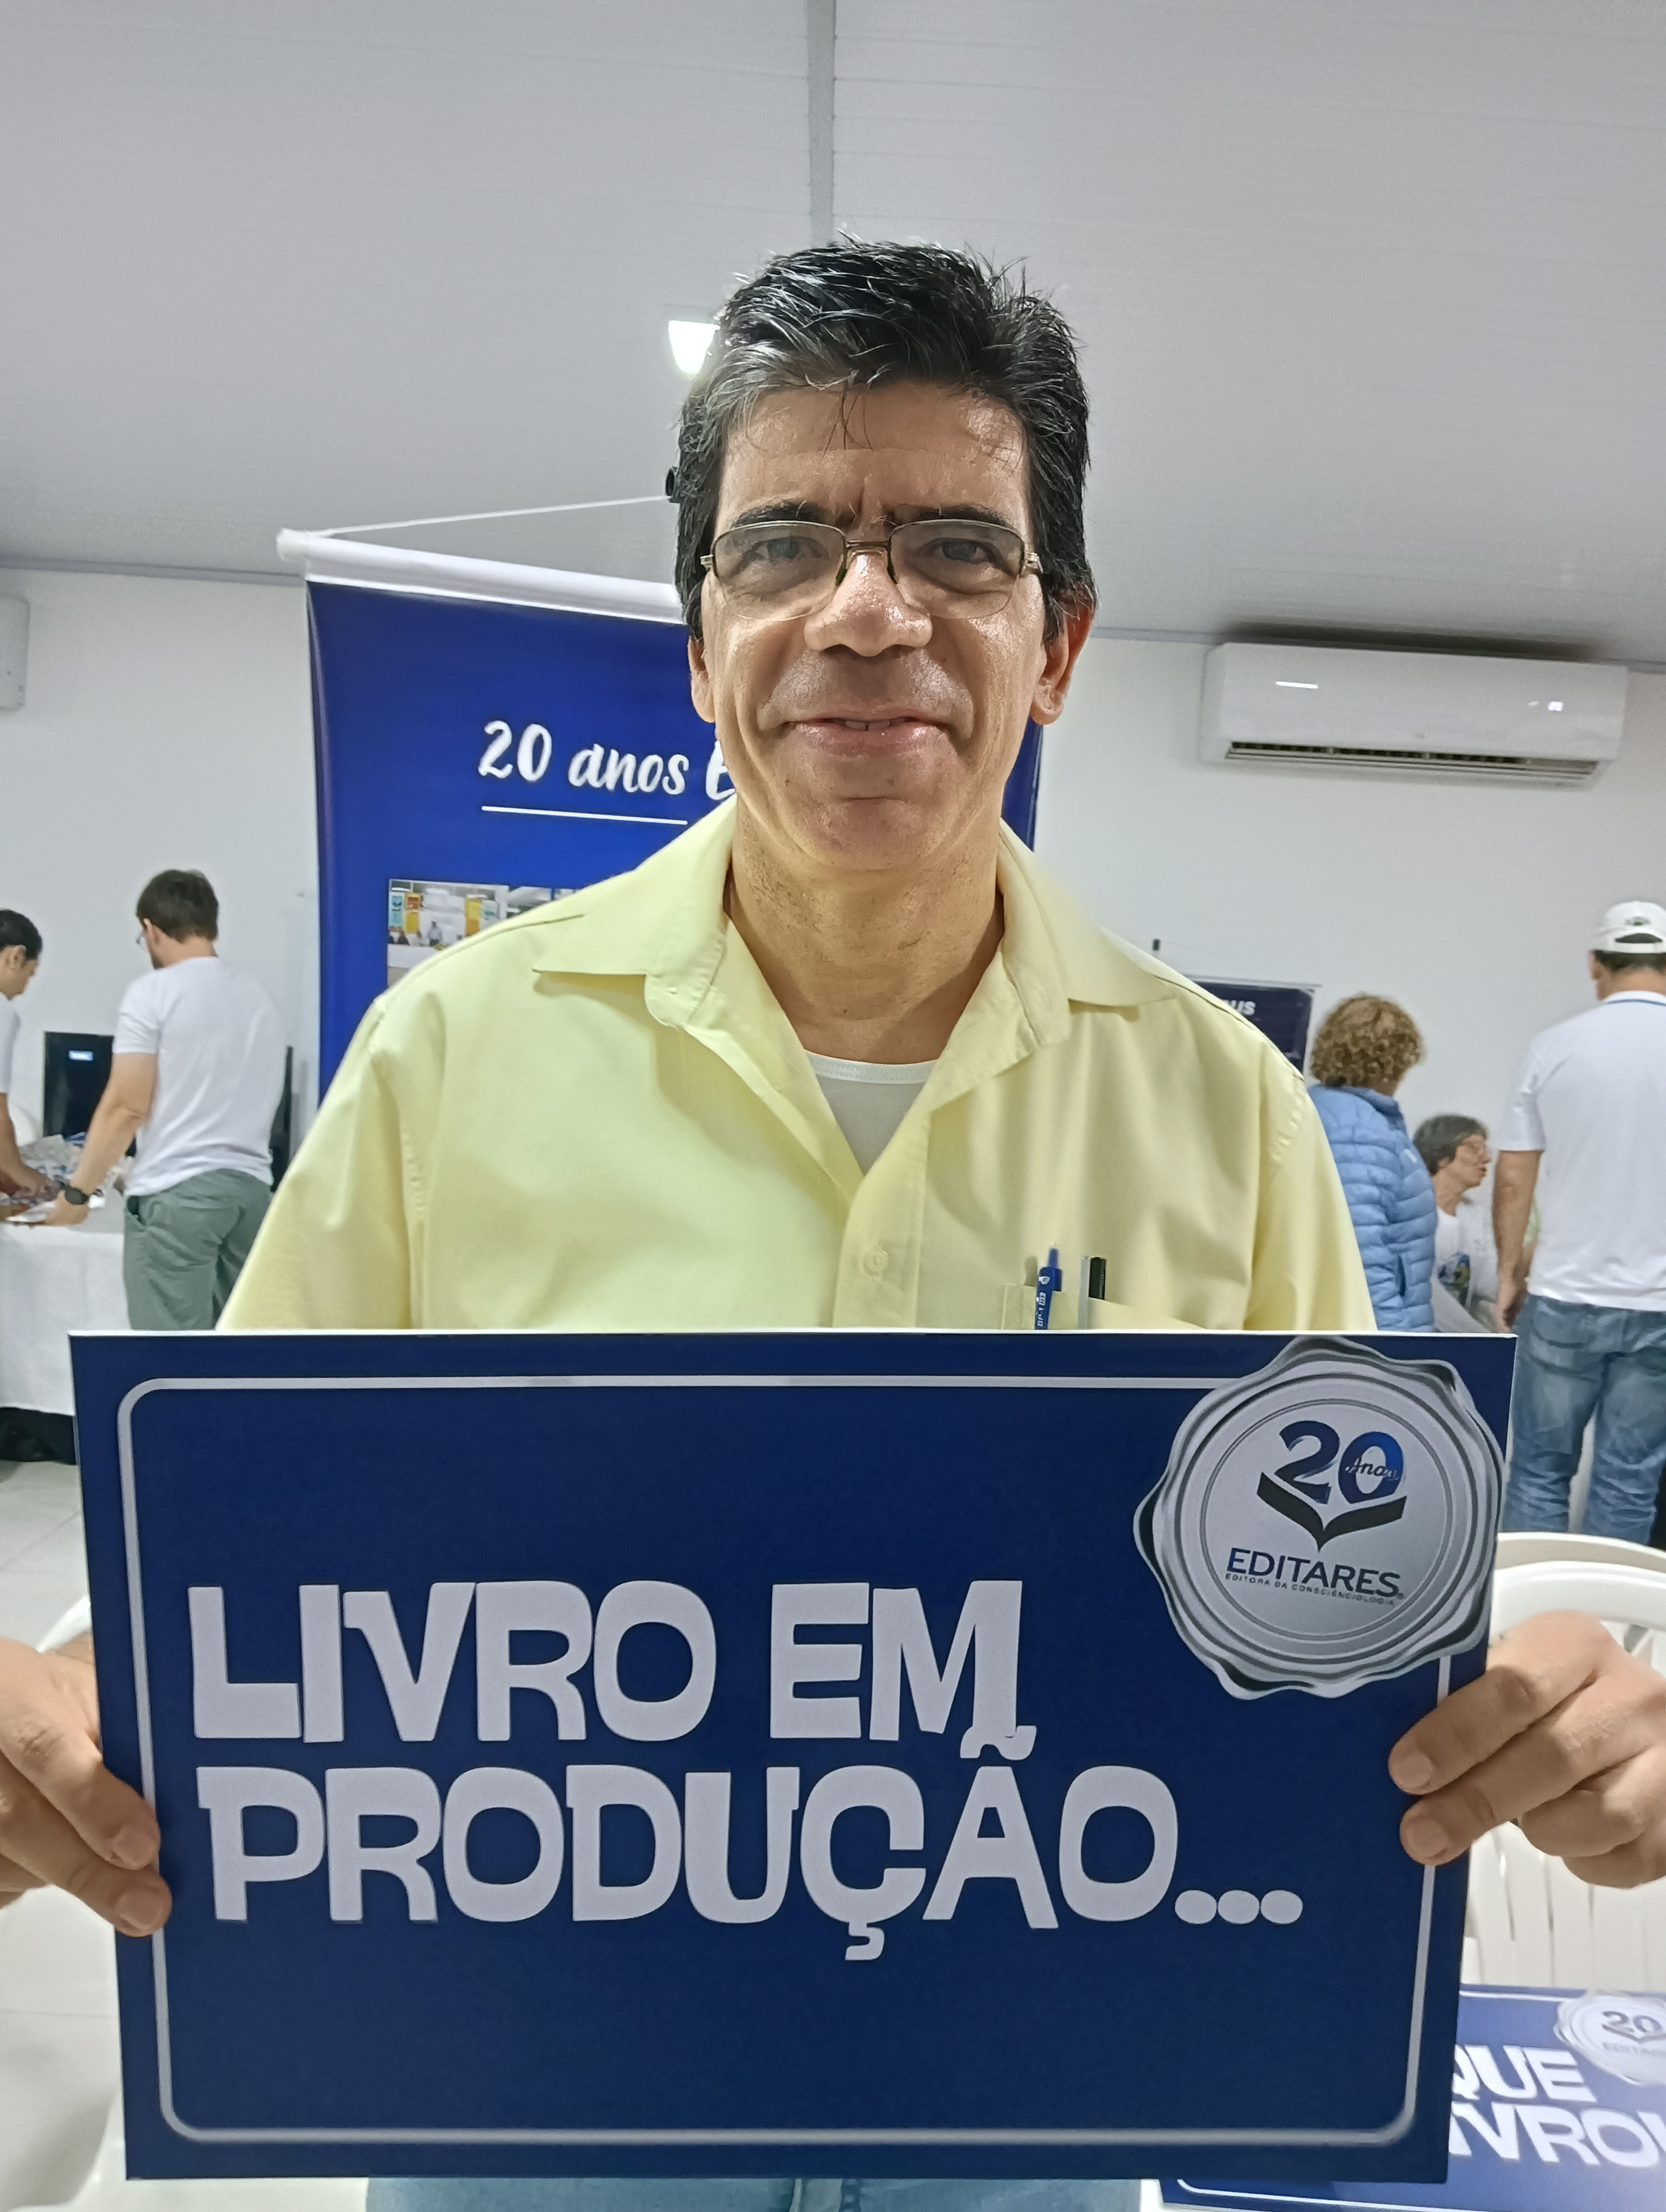
\includegraphics[height=5cm]{articles/resumo/fotos/materia2/IMG20241208144653.jpg}
  \end{minipage}\hfill
  \begin{minipage}[b]{0.55\textwidth}
    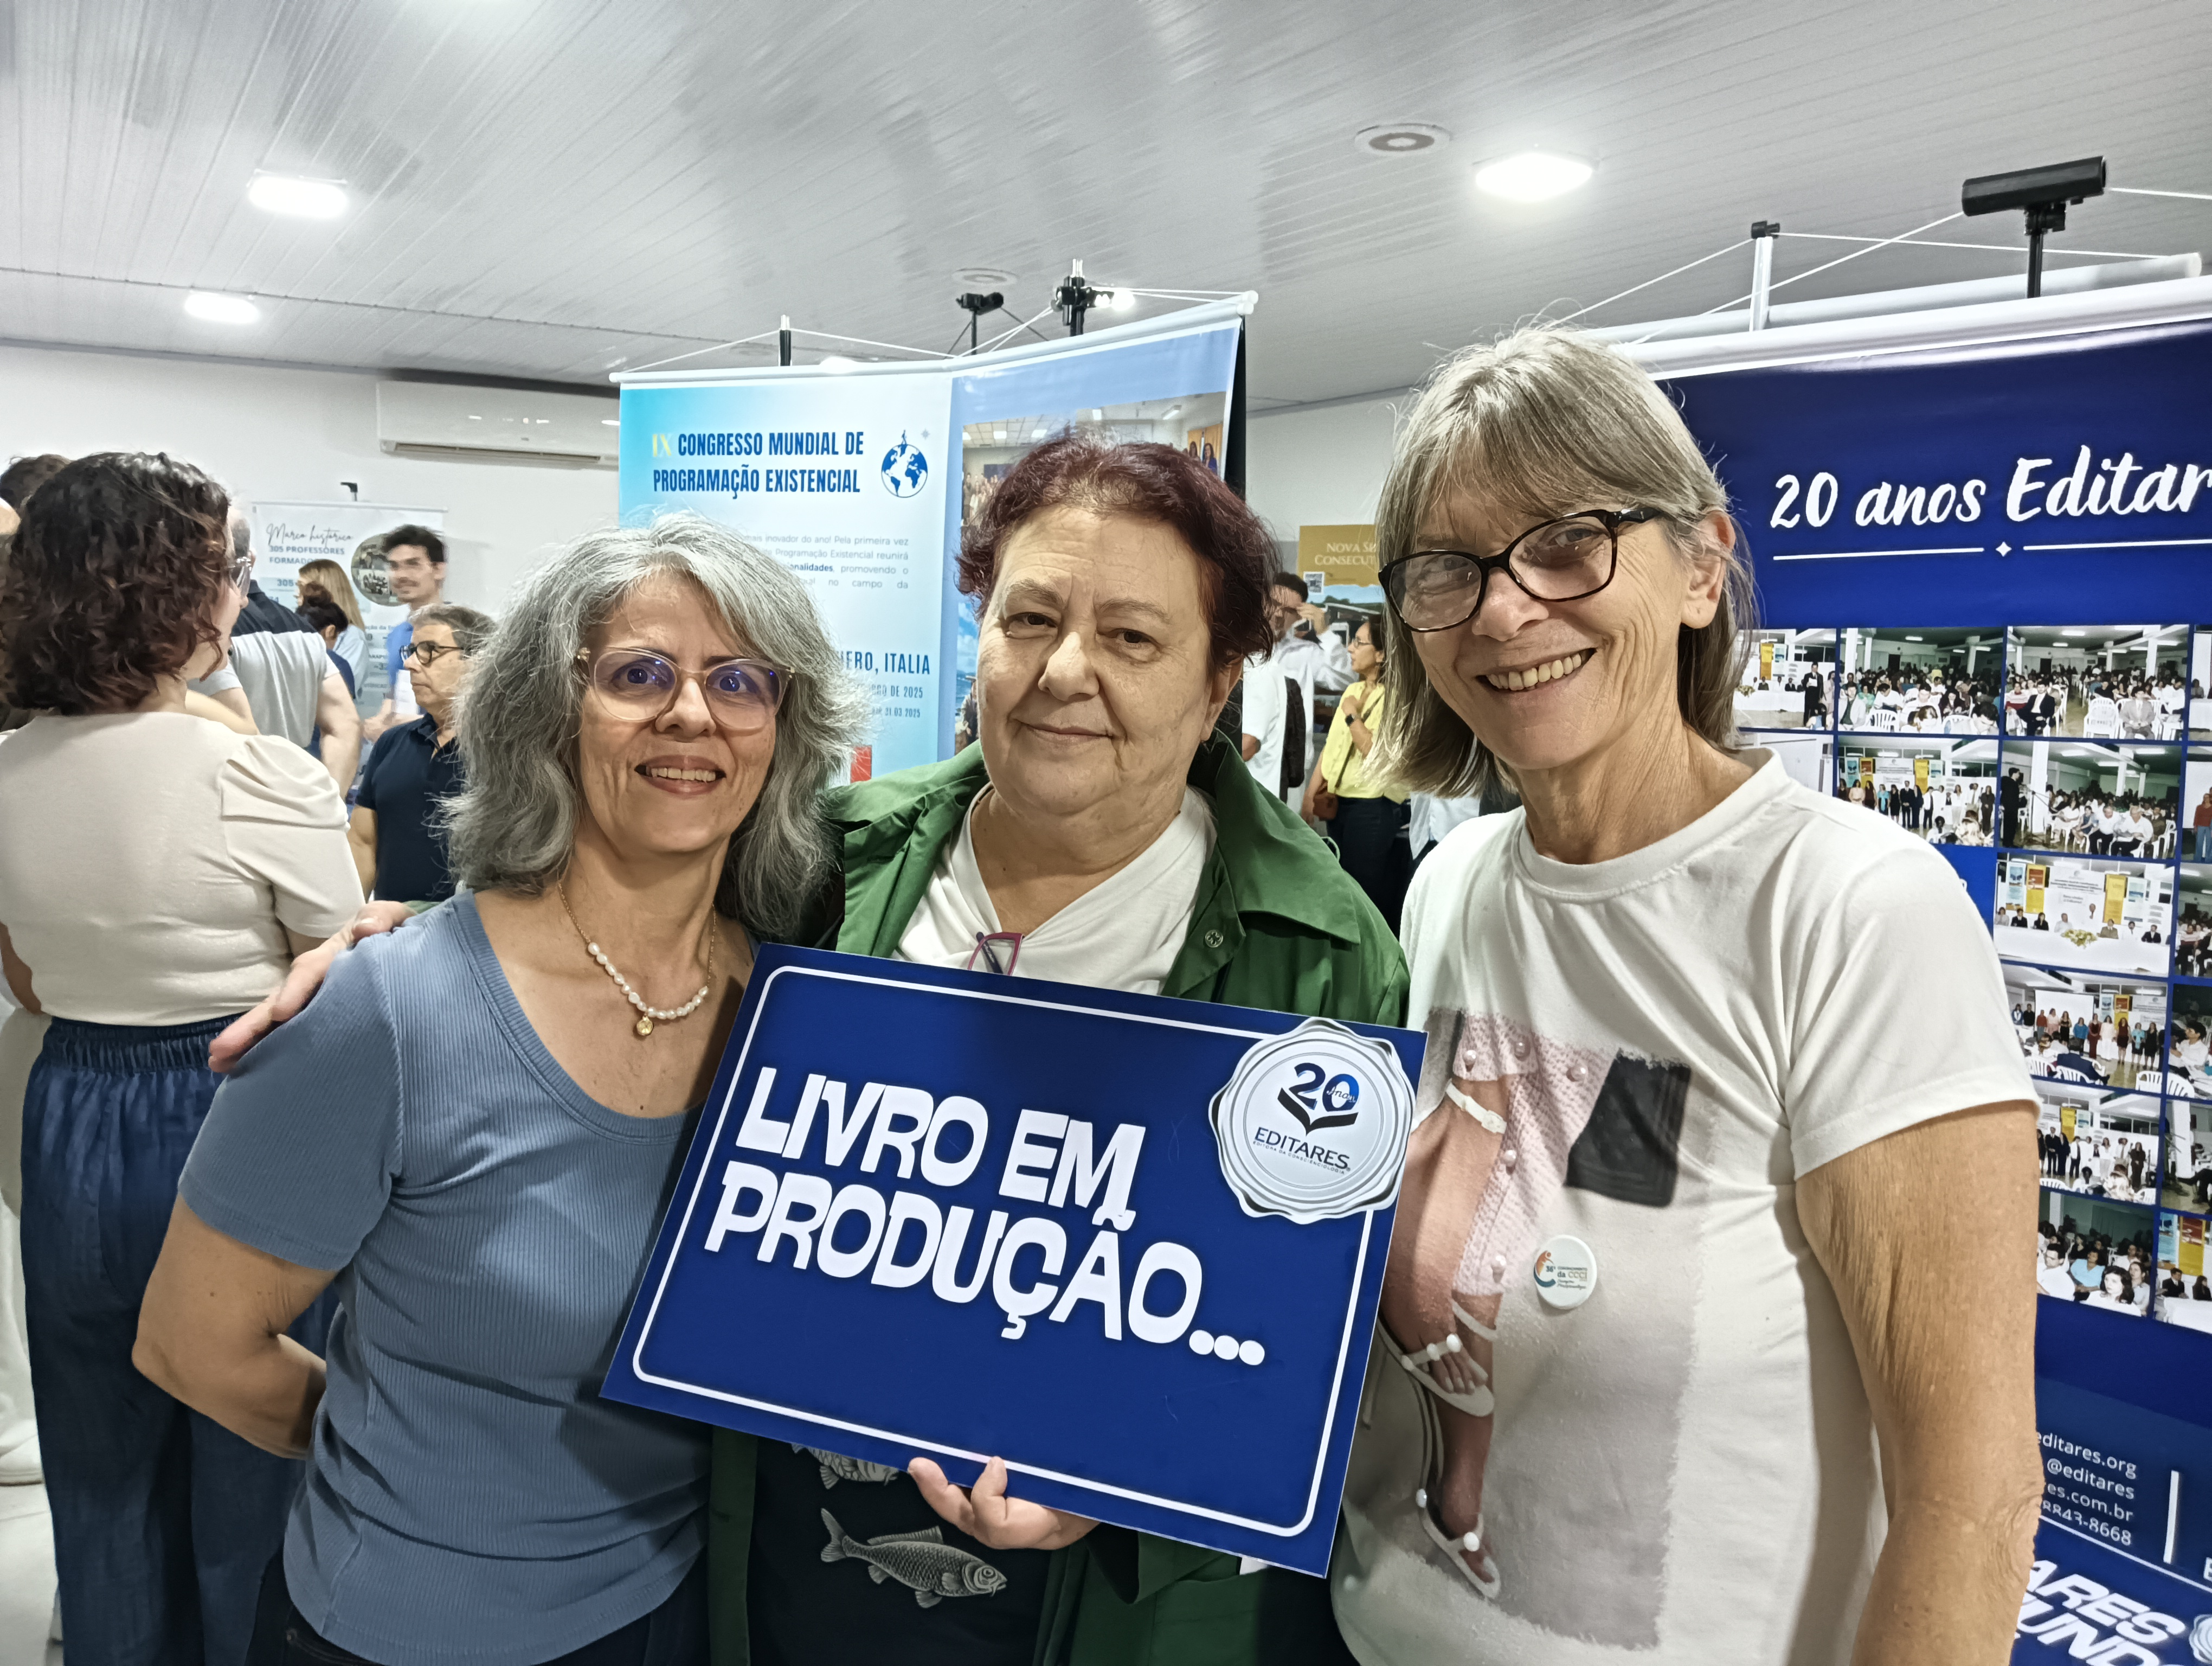
\includegraphics[height=5cm]{articles/resumo/fotos/materia2/IMG20241208155101.jpg}
  \end{minipage}

\coverart{../fundo-generico.png}

%{[}MURAL/MOSAICO DE FOTOS{]} Fotos na pasta matéria 2\ldots{} as fotos podem ocupar 2 páginas



        
%    \end{multicols}
\end{document}

    \documentclass{gescons}

\genre {Resumo do Biênio}
\author{Ana Claudia Prado e Magda Stapf Amancio}
\authorrole{Coordenadoras Editares -- Biênio 2024-2025}
\title{Editares Conquista a Certificação Institucional da UNICIN em 2024}

\begin{document}
    \makeentrevistatitle
    %\maketitle

    %\fullwidthimage{fields}{b}

    %\coverart{back/editorial}
    \coverart{../fundo-generico.png}
    
%    \begin{multicols}{2}

%\begin{center}
%    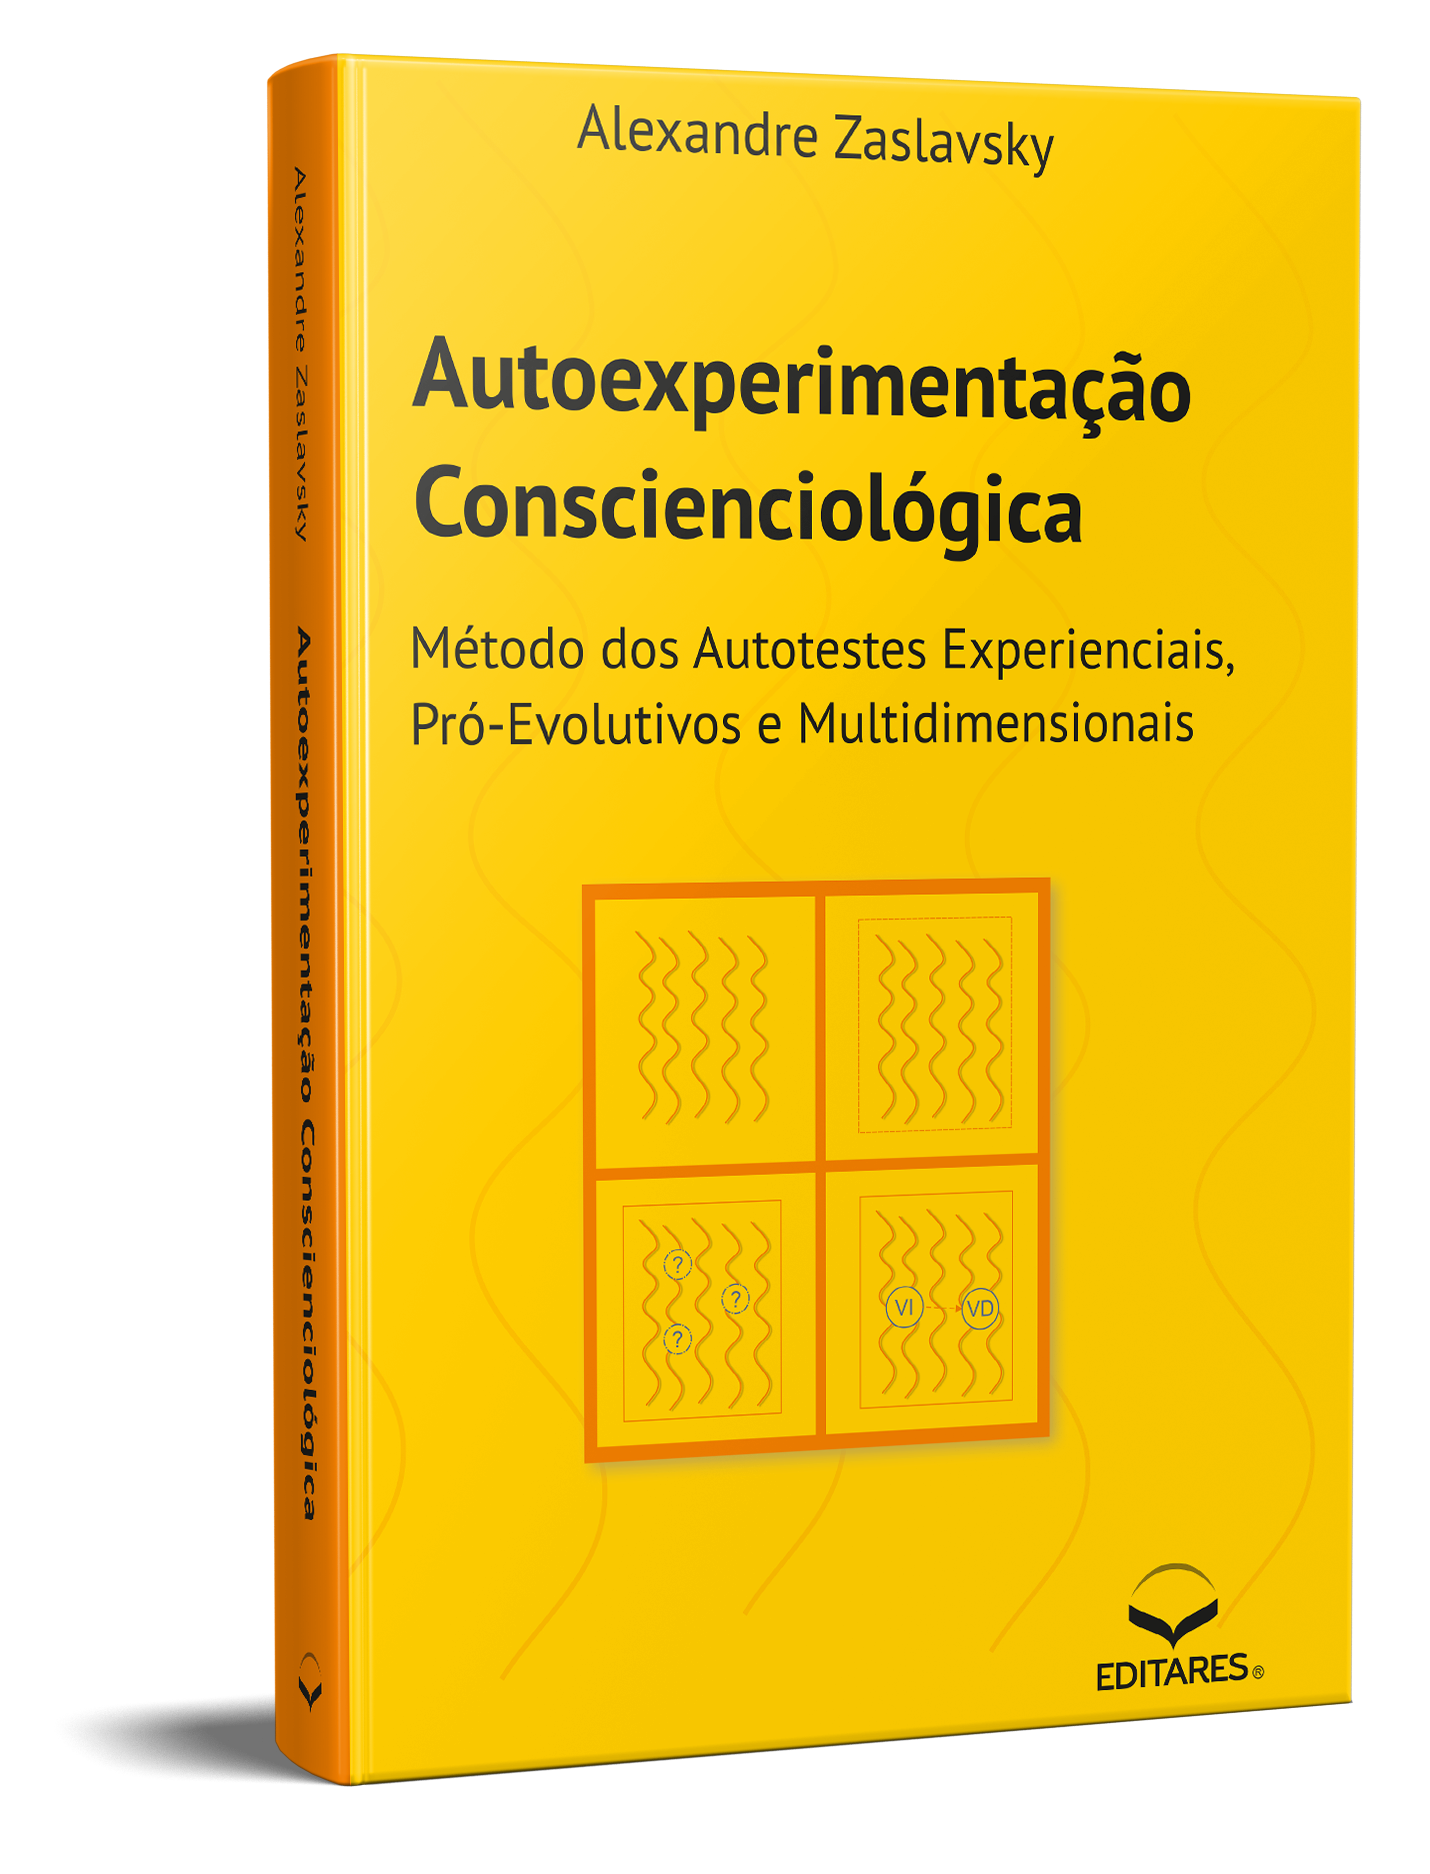
\includegraphics[width=4cm]{articles/entrevista/mockups/Alexandre-Zas.png}
%\end{center}


%\usepackage{graphicx}
%\usepackage{subcaption} % se quiser sublegendas

\begin{figure}[h]
  \centering
  \begin{subfigure}[b]{0.49\textwidth}
    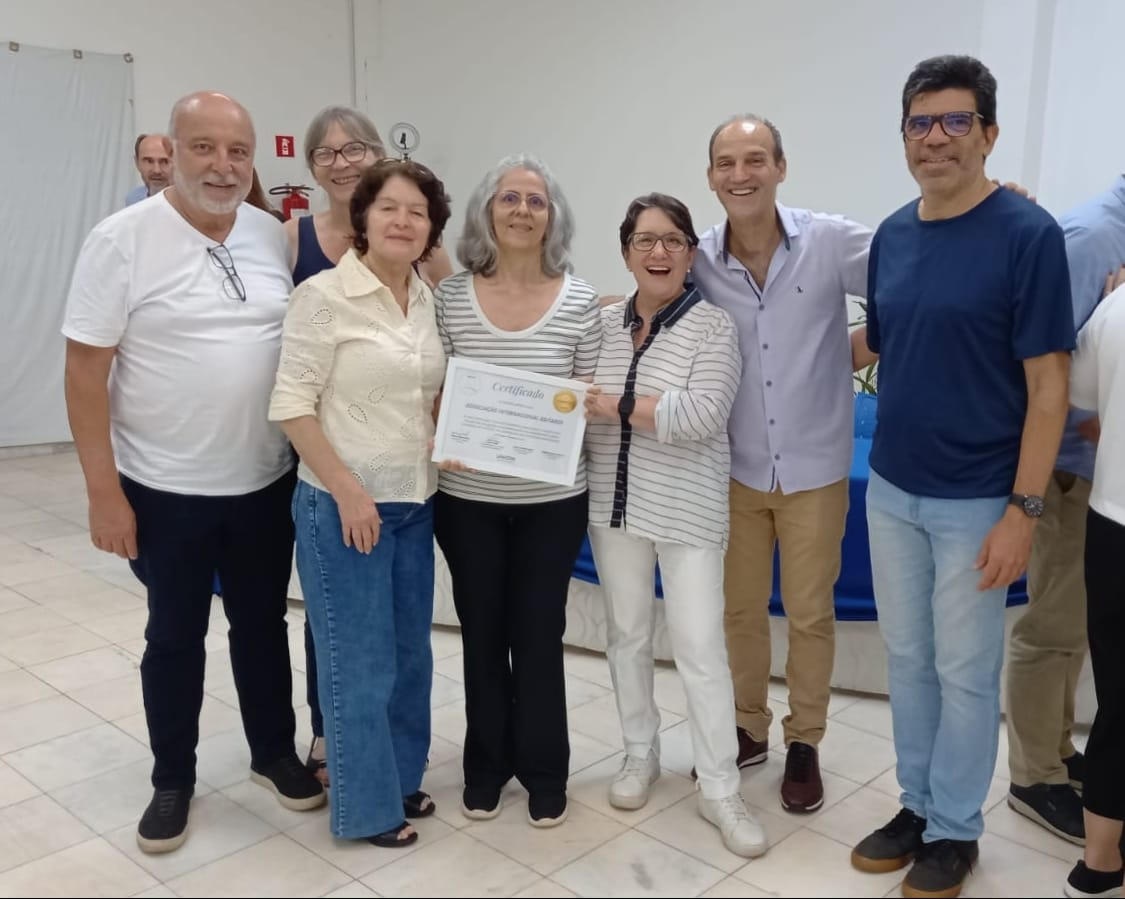
\includegraphics[height=60mm,keepaspectratio]{articles/resumo/fotos/materia3/d94f6571-cf63-48d2-976b-507cbf8cafc5.jpg}
\end{subfigure}
\begin{subfigure}[b]{0.49\textwidth}
    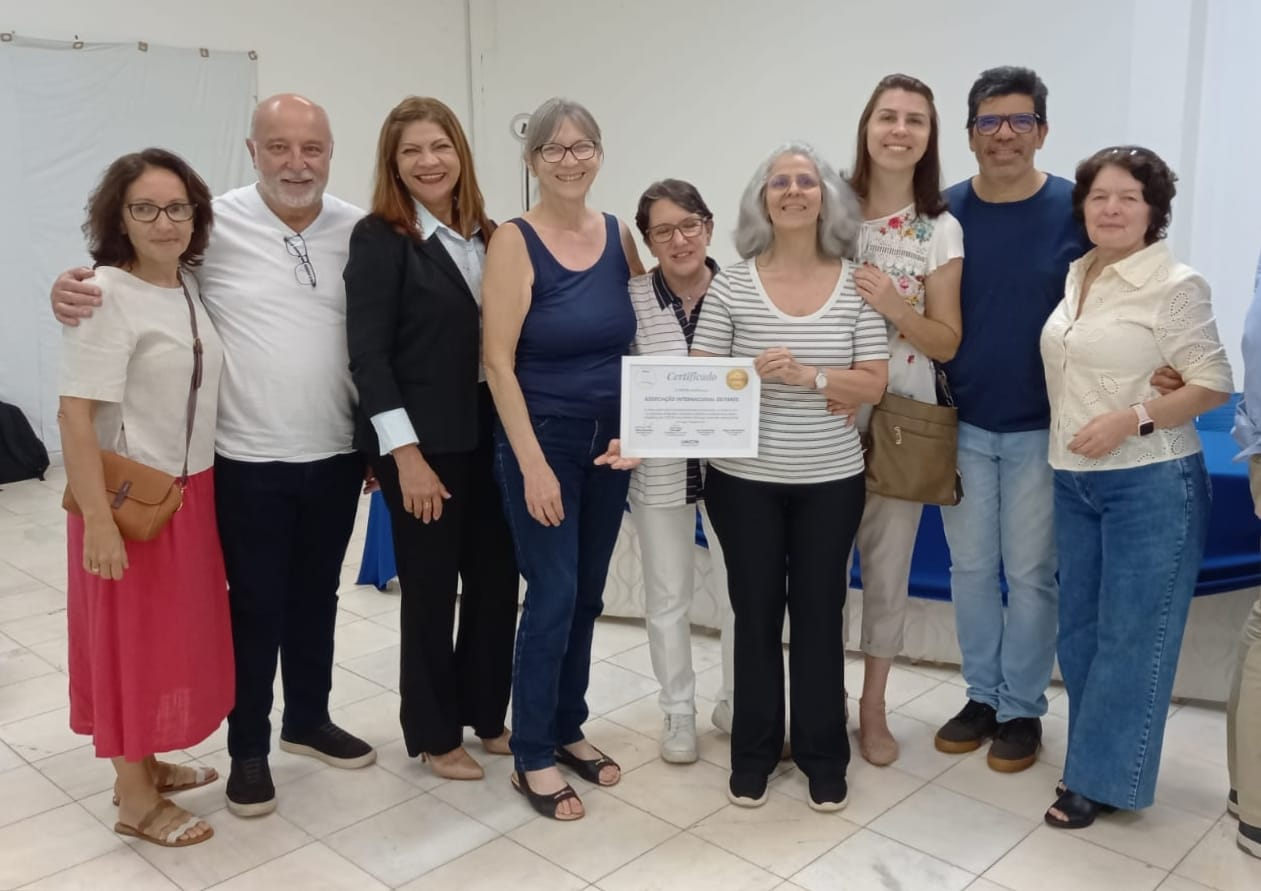
\includegraphics[height=60mm,keepaspectratio]{articles/resumo/fotos/materia3/06eb15bb-01a3-43d5-84e2-67f62c13a53e.jpg}
  \end{subfigure}
\end{figure}


%\noindent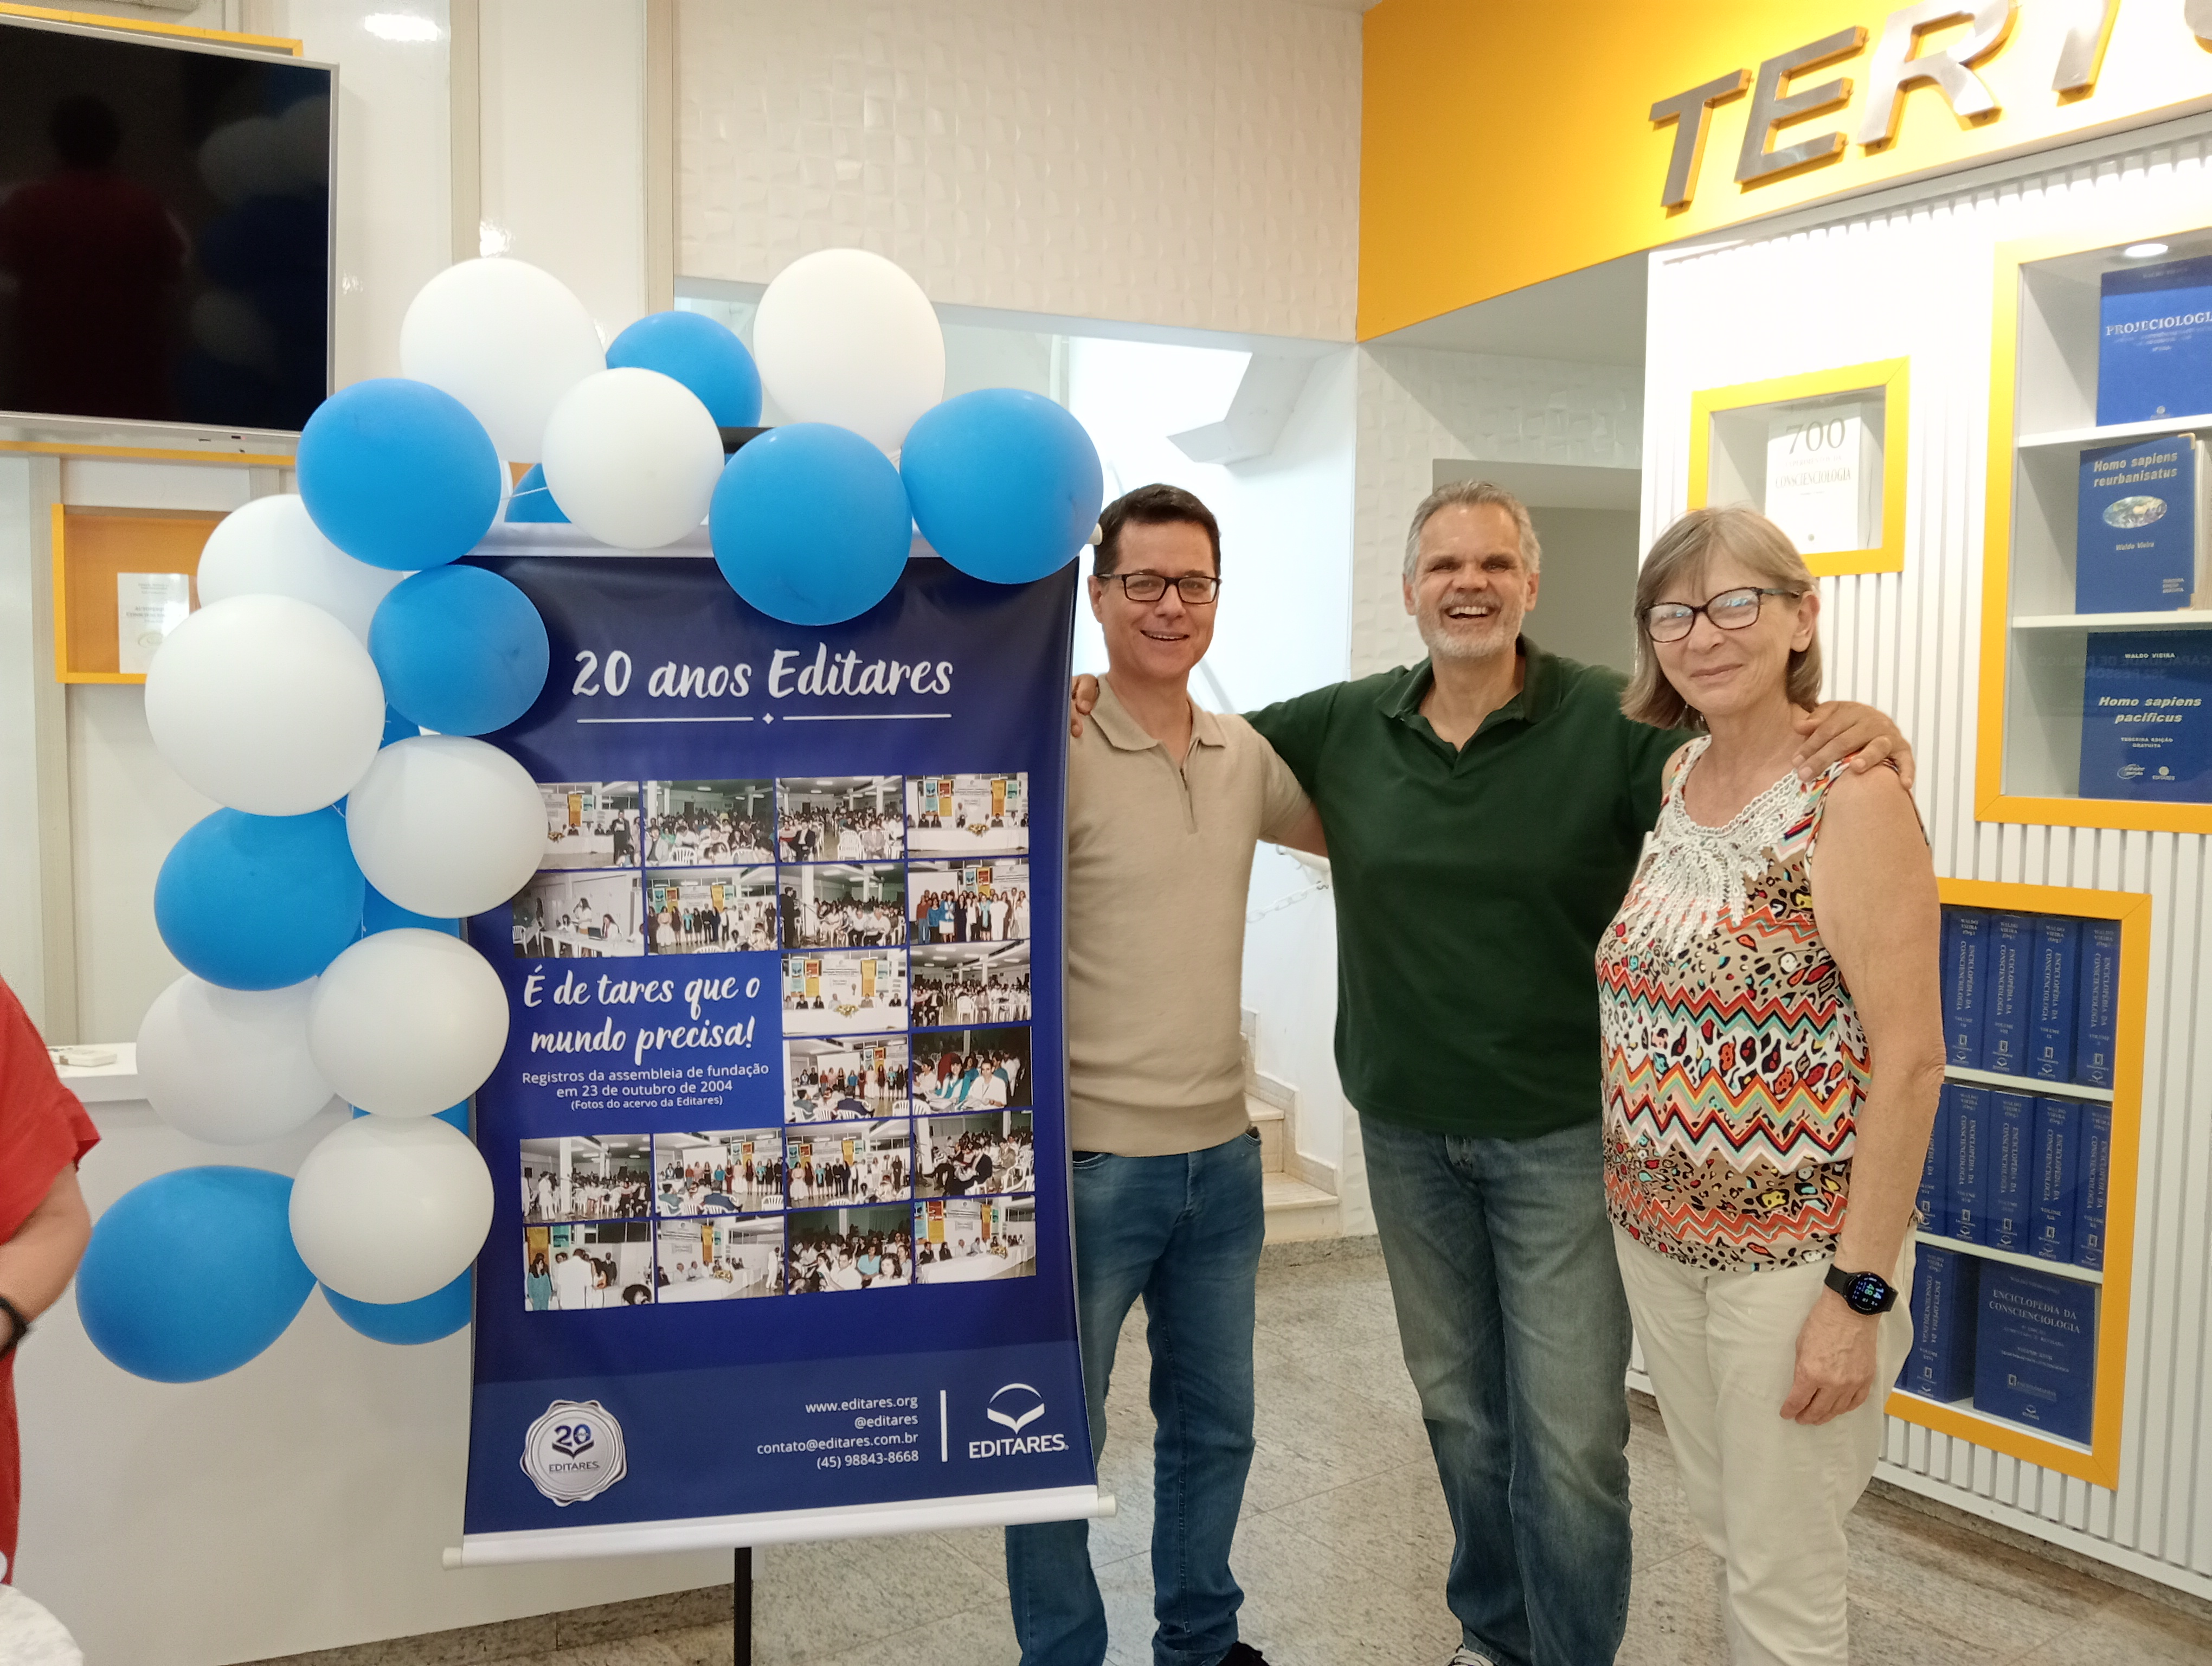
\includegraphics[width=9cm, height=9cm]{articles/resumo/fotos/materia1/IMG20241023144802.jpg}

A Editares recebeu, pela segunda vez, a \emph{Certificação Institucional
da UNICIN,} após avaliação realizada em 2024. A primeira certificação
ocorreu em 2019. Esse reconhecimento reforça o alinhamento da IC à
maxiproéxis grupal da \emph{Comunidade Conscienciológica Cosmoética
Internacional} (CCCI) e ao compromisso contínuo com a
interassistencialidade tarística.

A \emph{Certificação Institucional} promovida pela UNICIN não tem
caráter técnico ou legal como as certificações normativas nacionais, mas
representa um \emph{aval grupal,} validando a atuação funcional e
interassistencial da IC dentro do fluxo da CCCI.

O processo é coordenado pelo \emph{Comitê Conscienciocêntrico da
UNICIN,} que envia um formulário-padrão às \emph{Instituições
Conscienciocêntricas} (ICs). As respostas são analisadas por conselhos
especializados:

\begin{itemize}
\item
  Conselho de Interassistência Jurídica da Conscienciologia (CIAJUC)
\item
  Conselho Intercientífico
\item
  Conselho de Parapedagogia
\item
  Conselho Intervoluntariado
\item
  Conselho de Interassistência em Economia, Finanças e Orientação Fiscal
  (CIEFFI)
\end{itemize}

A certificação visa verificar o grau de maturidade institucional em
aspectos como gestão, interassistência, parapedagogia, voluntariado e
sustentabilidade organizacional, sempre sob a ótica dos princípios
conscienciais.

A conquista da certificação pela Editares em 2024 reflete o esforço
coletivo dos voluntários e a consolidação do trabalho editorial
tarístico, contribuindo com a reurbex planetária e a expansão da
Conscienciologia.

Editares agradece à UNICIN e aos conselhos envolvidos pela seriedade no
processo, e renova seu compromisso com a interassistência tarística e o
fortalecimento da maxiproéxis grupal.


%v \textbf{{[}INSERIR UMA DAS FOTOS DA PASTA ``MATÉRIA 3''{]}}



%\noindent
\includegraphics[width=9cm, height=9cm]{articles/resumo/fotos/materia1/IMG20241023143149.jpg}
        
%    \end{multicols}
\end{document}

    \documentclass{gescons}

\genre {Resumo do Biênio}
\author{Por Luziânia Medeiros e Paulo Abrantes}
\title{Conscienciologia em Expansão: Distribuição de Publicações no Japão e Europa}

\begin{document}
    \makeentrevistatitle
    %\maketitle

    %\fullwidthimage{fields}{b}

    %\coverart{back/editorial}
    \coverart{../fundo-generico.png}
    
%    \begin{multicols}{2}

%\begin{center}
%    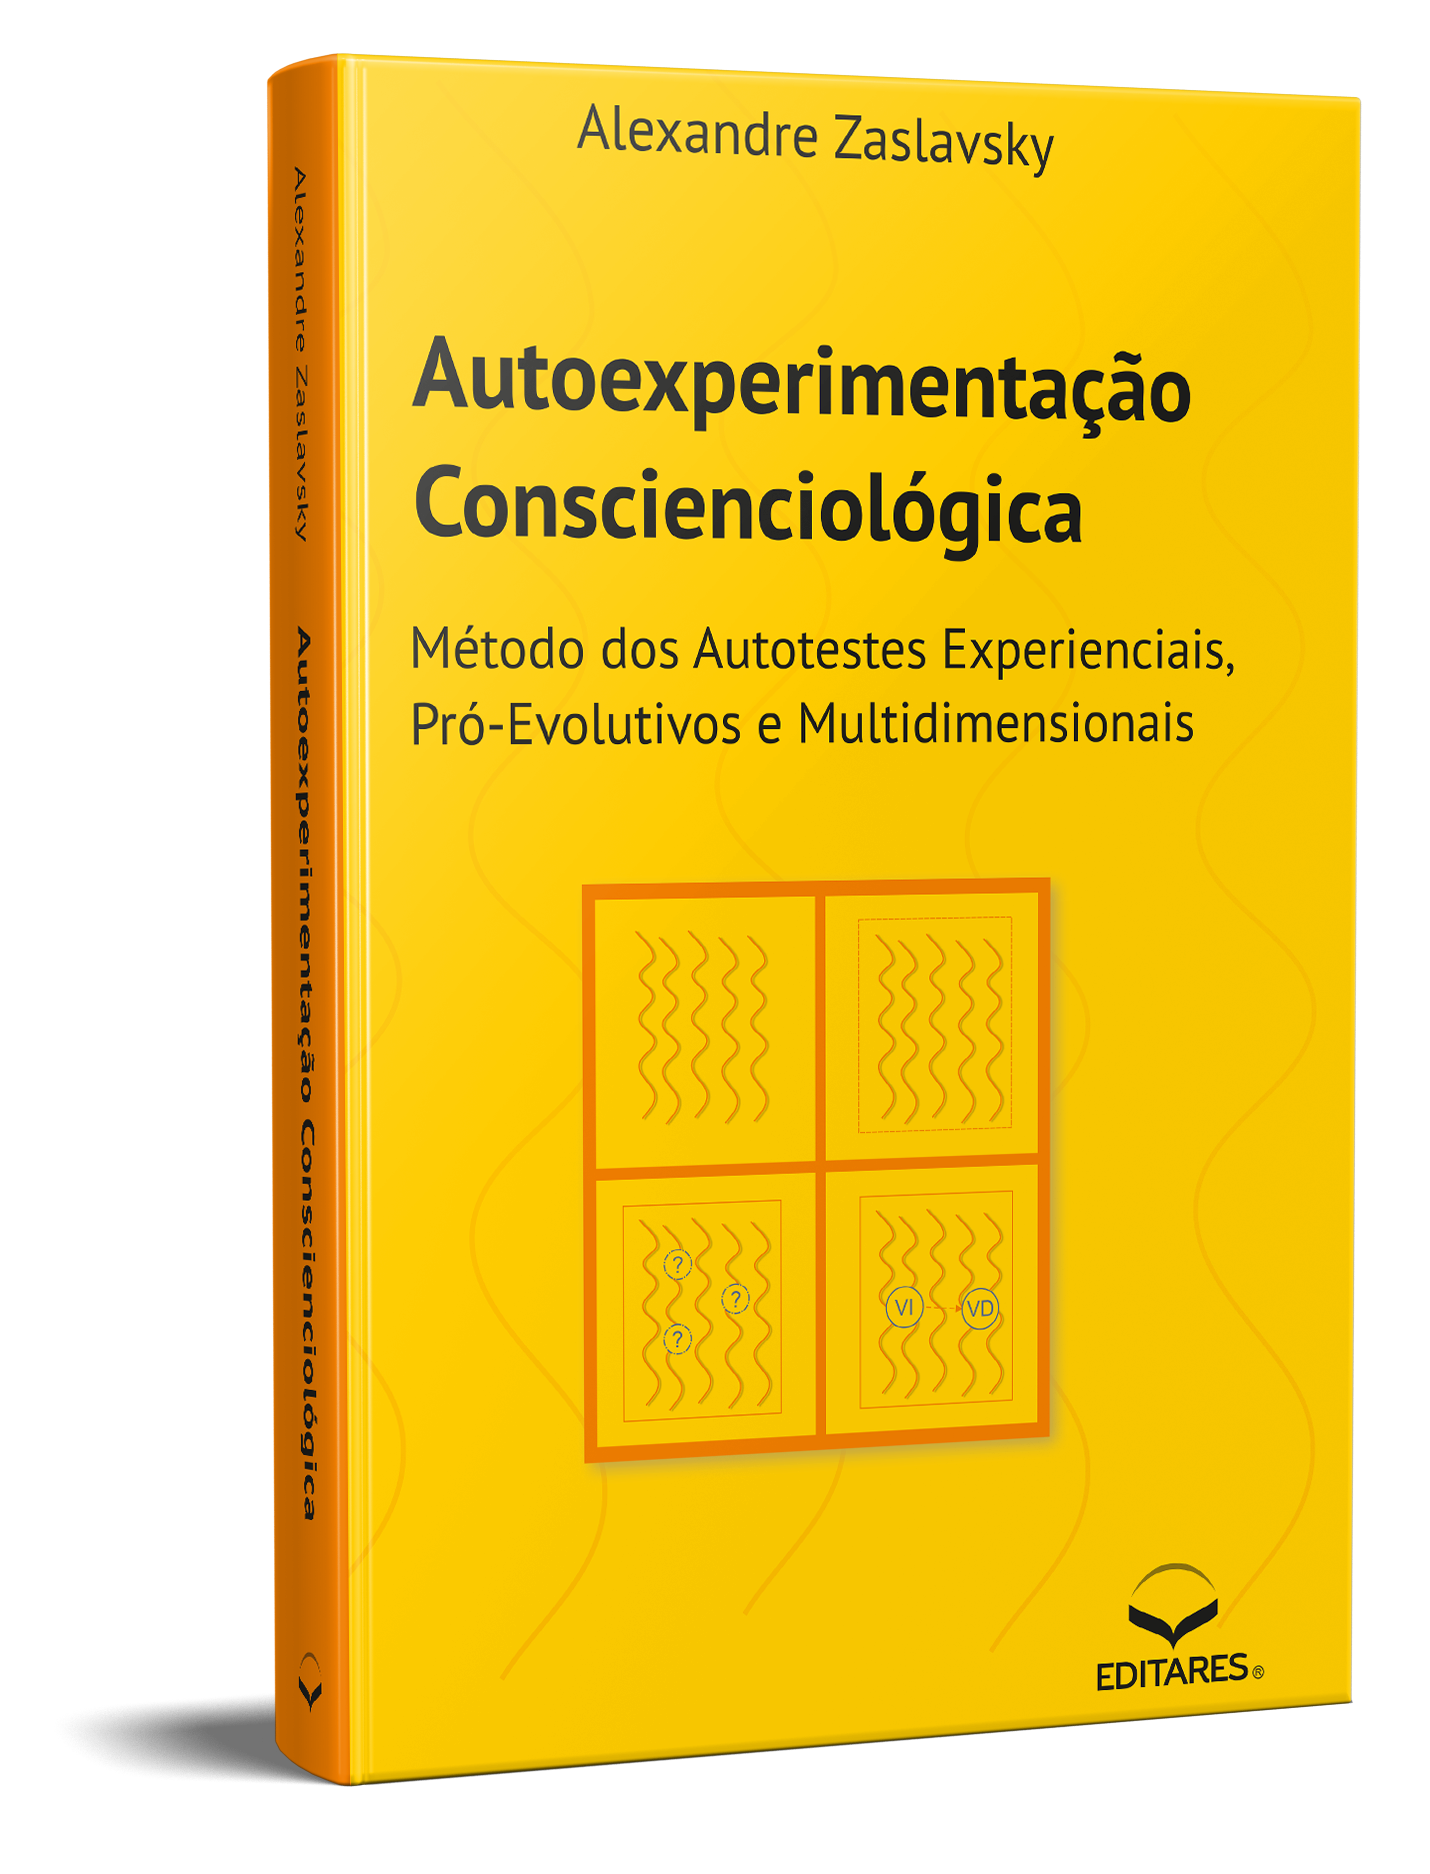
\includegraphics[width=4cm]{articles/entrevista/mockups/Alexandre-Zas.png}
%\end{center}


% \subsection*{Coordenadores da Expedição Paracientífica Expo 2025 Osaka}

A \emph{Expedição Paracientífica Expo 2025 Osaka} consistiu numa viagem técnica grupal, planejada em detalhes durante 2 anos, incluindo instrumentos de registro e documentação para coleta, sistematização, discussão, aprofundamento e síntese dos achados e parachados. Tudo isso visando pensar o \emph{Megacentro Cultural Holoteca} em ambiente universalista, pacífico e multicultural de uma Expo Mundial.

\subsection*{Gestação de publicações}

Para fazermos a interlocução com o público da Expo, observou-se a necessidade de apresentar a Cognópolis, a neociência Conscienciologia, seu propositor e pesquisadores, e os principais projetos, dentre eles o Jovem Pesquisador e o projeto do Megacentro Cultural Holoteca. Daí nasceu o projeto \emph{Holothecology Supplement}, \textbf{primeira versão} da revista em inglês.

Parte da equipe da Expedição estava há 1 ano e meio trabalhando no projeto do dicionário de termos da Conscienciologia em japonês. Sugerimos à equipe avaliar a possibilidade de publicar a primeira edição gratuita com termos produzidos até o momento, em formato de miniglossário, para ser distribuído entre os japoneses, presenteando-os com neovocábulos no idioma local. A equipe da Nipoteca da Holoteca aceitou prontamente o desafio e \textbf{fez a obra acontecer em 2 meses.}

\subsection*{A força do grupo: financiamento e distribuição das publicações}

A produção dessas publicações estava a todo vapor, porém havia um desafio: como financiar as impressões. Daí surgiu a ideia de captação por meio de um item colecionável, uma edição limitada da moeda comemorativa da Expedição. As doações ganharam força e o recurso arrecadado possibilitou a impressão de \textbf{1000 revistas e 500 mini-glossários.} Essa realização foi grupal, voluntária e com o propósito de divulgar as ideias da Conscienciologia para o público internacional mais amplo.

O material chegou há tempo de ser levado por alguns pesquisadores que estavam de viagem para vários países da Europa, em curso itinerante do \emph{Cosmovisão} promovido pela Assinvéxis. Foram disponibilizados dezenas de exemplares da revista \emph{Holothecology,} distribuídos em países como Inglaterra, França, Áustria e Suíça. Segundo relatos, a revista ajudou a criar pontes de interlocução em diferentes contextos ao longo da viagem. \textbf{A união faz a força!}

\subsection*{Balanço e prospectivas}

Distribuímos no Japão 260 \emph{Miniglossários}, 215 \emph{Holothecology}, 36 \emph{Our Evolution}, 2 \emph{Léxicos de Ortopensatas} e 1 \emph{Manual dos Megapensenes Trivocabulares}. As publicações foram deixadas em 8 cidades do Japão, incluindo bibliotecas, sebos, universidades e instituições, e na Expo circularam em pelo menos 43 pavilhões de países dos 5 continentes, e em pavilhões de instituições internacionais como ONU, União Europeia, Cruz Vermelha e Bureau International des Expositions (BIE). Sem falar dos contatos espontâneos com japoneses em vários locais visitados no Japão e com pessoas de várias nacionalidades que visitavam a Expo.

Foram estabelecidos vários canais de contatos com pessoas e instituições, verdadeiras \textbf{pontes interassistenciais} de natureza variada a serem cultivadas e desenvolvidas ao longo dos próximos anos.

Essas iniciativas fortalecem o avanço do Megacentro Cultural Holoteca, um megaempreendimento grupal prioritário, de natureza policármica, abrangente, e que contribuirá para a consolidação da Conscienciologia no planeta.

%v \textbf{{[}INSERIR FOTOS DA PASTA MATÉRIA 4 - \emph{falta receber essas fotos}{]}}

%\noindent
\includegraphics[width=9cm, height=9cm]{articles/resumo/fotos/materia1/IMG20241023143149.jpg}
        
%    \end{multicols}
\end{document}

    \documentclass{gescons}

\genre {Resumo do Biênio}
\author{Ana Claudia Prado e~Magda Stapf Amancio}
\authorrole{Coordenadoras Gerais da Editares}
\title{Da Ideia do Autor às Mãos do Leitor: o~Fluxo Editorial Conscienciológico}

\begin{document}
    \makeentrevistatitle
    %\maketitle

    %\fullwidthimage{fields}{b}

    %\coverart{back/editorial}
    \coverart{../fundo-generico.png}
    
%    \begin{multicols}{2}

%\begin{center}
%    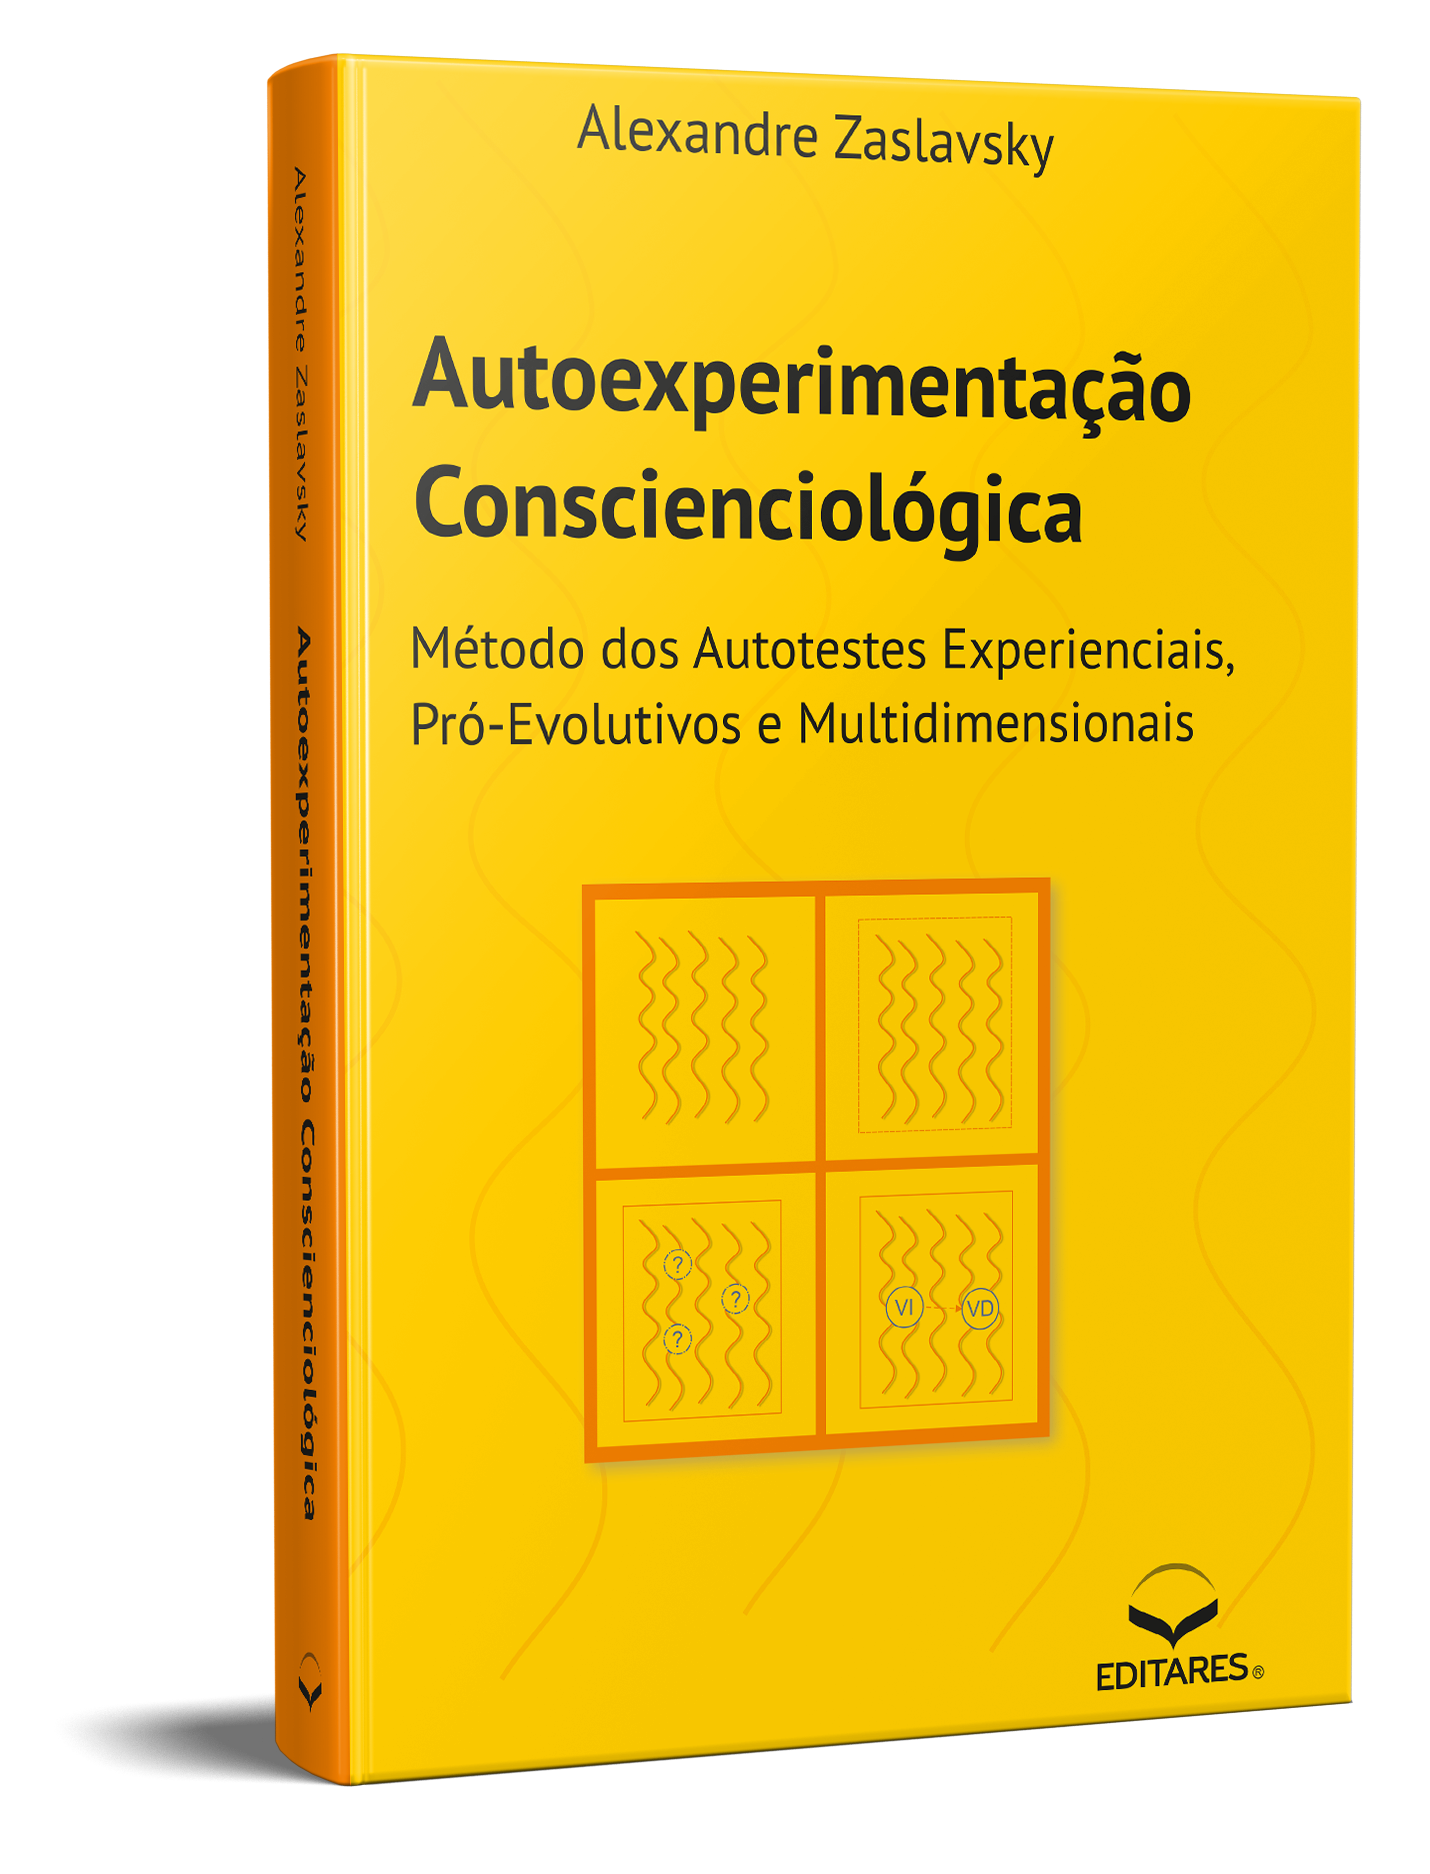
\includegraphics[width=4cm]{articles/entrevista/mockups/Alexandre-Zas.png}
%\end{center}

Publicar um livro não é~apenas escrever. Na Editares, cada obra passa por um processo integrado que alia rigor editorial, trabalho voluntário e~compromisso interassistencial tarístico para \textbf{garantir qualidade e~relevância} antes de chegar ao leitor.

O fluxo editorial começa com o~envio dos originais textuais pelo autor para o~\emph{e-mail} da Editares. Em seguida, o~material é~inserido na plataforma \emph{Trello Editorial} e~submetido à~pré-análise por uma equipe voluntária, que analisa conteúdo, estrutura e~a~forma. Quando necessário, o~texto retorna ao autor para melhorias até estar pronto para avançar.

Com a~aprovação da pré-análise, o~material textual ingressa no fluxo formal de produção editorial que contempla parecer técnico, assinatura do termo de cessão de direitos autorais e~revisões linguístico-textual e~de conteúdo e~forma --- conhecidas como \emph{Confor.} Durante esta etapa, o~editor e~revisores especializados trabalham em parceria com o~autor, garantindo autenticidade e~qualidade técnica.

Com o~texto finalizado, o~livro passa para a~diagramação, momento em que o~conteúdo ganha forma gráfica, tornando-se fluido e~agradável à~leitura. O~autor pode optar pela diagramação voluntária da Editares ou contratar um profissional externo. Antes de seguir para a~impressão, uma prova física é~cuidadosamente revisada para assegurar o~acabamento.

Após a~definição do orçamento e~da tiragem, a~obra é~encaminhada para a~gráfica. Paralelamente, a~equipe de comunicação prepara o~lançamento do livro, um \textbf{momento de celebração da conquista do autor} e~de início da circulação da obra entre leitores em geral.

Mais do que um produto editorial, cada título publicado pela Editares representa a~\textbf{difusão da Conscienciologia,} fortalecendo a~interassistência e~promovendo o~crescimento evolutivo de todos os envolvidos.

% \textbf{FLUXO EDITORIAL DE OBRA CONSCIENCIOLÓGICA}

%\emph{{[}IMAGEM DO FLUXO EDITORIAL ESTÁ NA PASTA FLUXO EDITORIAL{]}}

% \begin{center}
%     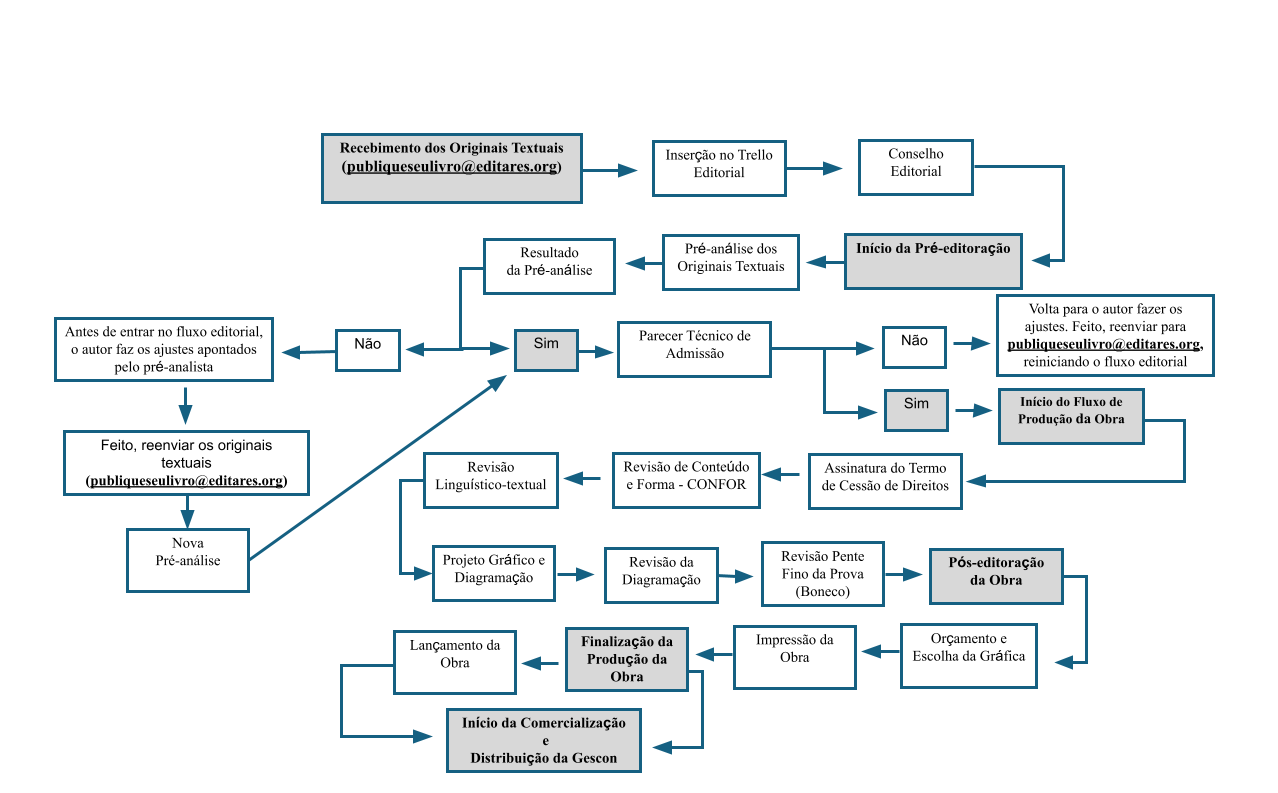
\includegraphics[width=16cm]{articles/resumo/fotos/fluxo-editorial/fluxo-editorial-artigo.png}
% \end{center}

\begin{figure}[h]
  \centering
  \caption*{Fluxo editorial de obra conscienciológica.} % sem numeração
  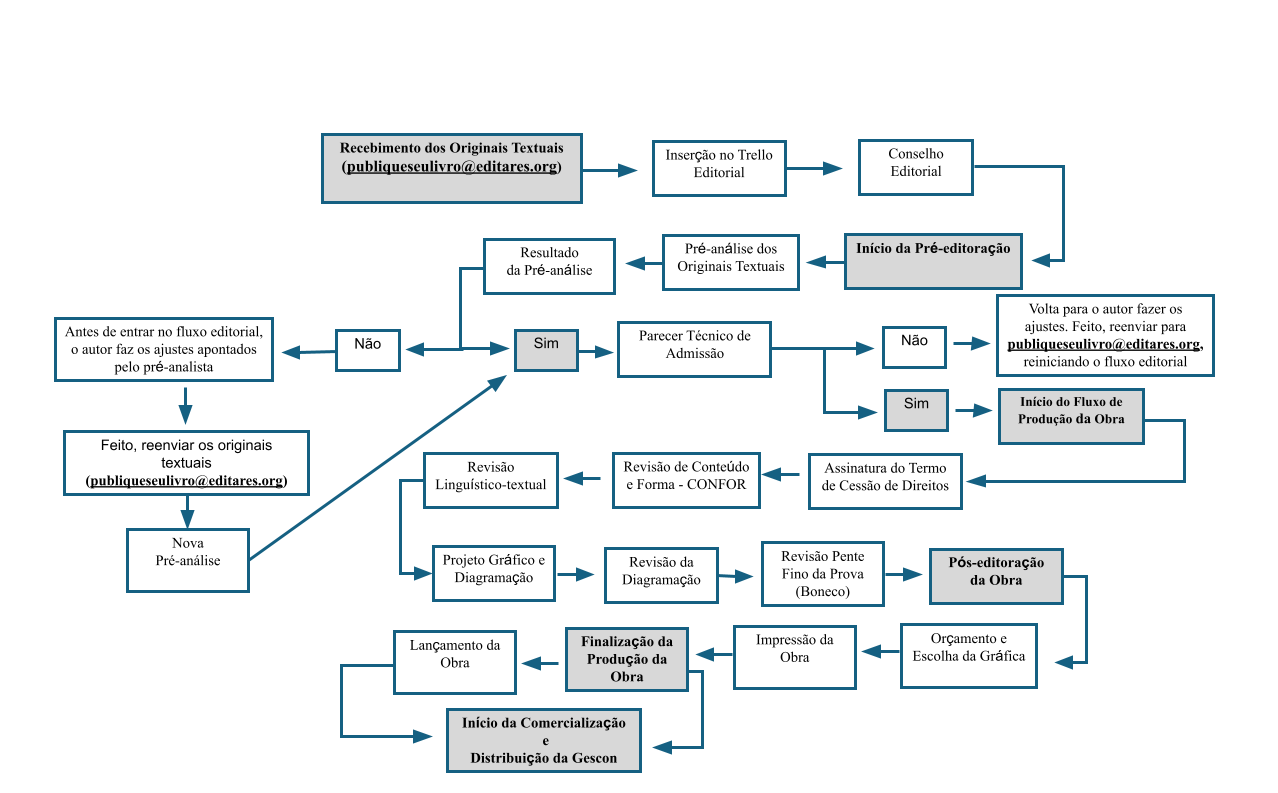
\includegraphics[width=18cm]{articles/resumo/fotos/fluxo-editorial/fluxo-editorial-artigo.png}
\end{figure}


%\noindent
\includegraphics[width=9cm, height=9cm]{articles/resumo/fotos/materia1/IMG20241023143149.jpg}
        
%    \end{multicols}
\end{document}

    \documentclass{gescons}

\genre {Resumo do Biênio}
\author{Amanda Vieira}
\title{Números do Biênio}

\begin{document}
    \makeentrevistatitle
    %\maketitle

    %\fullwidthimage{fields}{b}

    %\coverart{back/editorial}
    \coverart{../fundo-generico.png}
    
%    \begin{multicols}{2}

\section*{Lançamentos de obras em Português}

\begin{longtable}[]{@{}
  >{\raggedright\arraybackslash}p{(\linewidth - 4\tabcolsep) * \real{0.6627}}
  >{\raggedright\arraybackslash}p{(\linewidth - 4\tabcolsep) * \real{0.2304}}
  >{\raggedright\arraybackslash}p{(\linewidth - 4\tabcolsep) * \real{0.1069}}@{}}
\toprule\noalign{}
\begin{minipage}[b]{\linewidth}\centering
\textbf{Título}
\end{minipage} & \begin{minipage}[b]{\linewidth}\centering
\textbf{Autor}
\end{minipage} & \begin{minipage}[b]{\linewidth}\centering
\textbf{Lançamento}
\end{minipage} \\
\hline
\begin{minipage}[b]{\linewidth}\raggedright
Autolegado Evolutivo
\end{minipage} & \begin{minipage}[b]{\linewidth}\raggedright
Haydée Melo
\end{minipage} & \begin{minipage}[b]{\linewidth}\raggedright
06/04/2024
\end{minipage} \\
\hline
\begin{minipage}[b]{\linewidth}\raggedright
Mutatis Mutandis: Teoria e Prática da Reciclagem Existencial
\end{minipage} & \begin{minipage}[b]{\linewidth}\raggedright
Luimara Schmit
\end{minipage} & \begin{minipage}[b]{\linewidth}\raggedright
10/08/2024
\end{minipage} \\
\hline
\begin{minipage}[b]{\linewidth}\raggedright
Megapensenes Trivocabulares Pró-evolutivos
\end{minipage} & \begin{minipage}[b]{\linewidth}\raggedright
Michel Chad
\end{minipage} & \begin{minipage}[b]{\linewidth}\raggedright
17/08/2024
\end{minipage} \\
\hline
\begin{minipage}[b]{\linewidth}\raggedright
Epicentrismo Consciencial: Casuísticas Recinológicas
\end{minipage} & \begin{minipage}[b]{\linewidth}\raggedright\addlinespace[2pt]
Ana Luiza Rezende e Mabel Teles
\end{minipage} & \begin{minipage}[b]{\linewidth}\raggedright
24/08/2024
\end{minipage} \\
\hline
\begin{minipage}[b]{\linewidth}\raggedright
Interassistência: Teoria e Prática sob a Ótica da Conscienciologia
\end{minipage} & \begin{minipage}[b]{\linewidth}\raggedright
Roberta Bouchardet
\end{minipage} & \begin{minipage}[b]{\linewidth}\raggedright
19/10/2024
\end{minipage} \\
\hline
\begin{minipage}[b]{\linewidth}\raggedright
Gratidão: Reconhecer, Expressar e Retribuir
\end{minipage} & \begin{minipage}[b]{\linewidth}\raggedright
Karine Brito
\end{minipage} & \begin{minipage}[b]{\linewidth}\raggedright
16/11/2024
\end{minipage} \\
\hline
\begin{minipage}[b]{\linewidth}\raggedright
Autoexperimentação Conscienciológica
\end{minipage} & \begin{minipage}[b]{\linewidth}\raggedright
Alexandre Zaslavsky
\end{minipage} & \begin{minipage}[b]{\linewidth}\raggedright
23/11/2024
\end{minipage} \\
\hline
\begin{minipage}[b]{\linewidth}\raggedright
O Calidoscópio da evolução consciencial
\end{minipage} & \begin{minipage}[b]{\linewidth}\raggedright
Maria Cristina Bassanesi
\end{minipage} & \begin{minipage}[b]{\linewidth}\raggedright
30/11/2024
\end{minipage} \\
\hline
\begin{minipage}[b]{\linewidth}\raggedright
Ortoprincípios Norteadores da Invéxis
\end{minipage} & \begin{minipage}[b]{\linewidth}\raggedright
Ricardo Rezende
\end{minipage} & \begin{minipage}[b]{\linewidth}\raggedright
07/10/2024
\end{minipage} \\
\hline
\begin{minipage}[b]{\linewidth}\raggedright
Ações Antifanatismo
\end{minipage} & \begin{minipage}[b]{\linewidth}\raggedright
Daniel Mamede
\end{minipage} & \begin{minipage}[b]{\linewidth}\raggedright
26/04/2025
\end{minipage} \\
\hline
\begin{minipage}[b]{\linewidth}\raggedright
Autoidentificação Proexológica
\end{minipage} & \begin{minipage}[b]{\linewidth}\raggedright
Ricardo Rezende
\end{minipage} & \begin{minipage}[b]{\linewidth}\raggedright
28/06/2025
\end{minipage} \\
\hline
\begin{minipage}[b]{\linewidth}\raggedright
Eitologia: Teática Inversiva
\end{minipage} & \begin{minipage}[b]{\linewidth}\raggedright
Pedro Borges
\end{minipage} & \begin{minipage}[b]{\linewidth}\raggedright
12/07/2025
\end{minipage} \\
\hline
\begin{minipage}[b]{\linewidth}\raggedright
Retomada de Tarefa: Reencontro com o Paradever Intermissivo
\end{minipage} & \begin{minipage}[b]{\linewidth}\raggedright
Ana Mazzonetto
\end{minipage} & \begin{minipage}[b]{\linewidth}\raggedright
19/07/2025
\end{minipage} \\
\hline
\begin{minipage}[b]{\linewidth}\raggedright
Autoinversão Existencial: Compreensão e Vivência
\end{minipage} & \begin{minipage}[b]{\linewidth}\raggedright
Paula Gabriella Barbosa
\end{minipage} & \begin{minipage}[b]{\linewidth}\raggedright
26/07/2025
\end{minipage} \\
\hline
\begin{minipage}[b]{\linewidth}\raggedright
Estado Vibracional: 100 Perguntas e Respostas
\end{minipage} & \begin{minipage}[b]{\linewidth}\raggedright
Victor Bolfe
\end{minipage} & \begin{minipage}[b]{\linewidth}\raggedright
02/08/2025
\end{minipage} \\
\hline
\begin{minipage}[b]{\linewidth}\raggedright
Migrações Proexológicas Internacionais
\end{minipage} & \begin{minipage}[b]{\linewidth}\raggedright
Virgínia Ruiz
\end{minipage} & \begin{minipage}[b]{\linewidth}\raggedright
30/08/2025
\end{minipage} \\
\hline
\begin{minipage}[b]{\linewidth}\raggedright
Autoconscientização Grafopensênica
\end{minipage} & \begin{minipage}[b]{\linewidth}\raggedright
Denise Paro
\end{minipage} & \begin{minipage}[b]{\linewidth}\raggedright
07/09/2025
\end{minipage} \\
\hline
\begin{minipage}[b]{\linewidth}\raggedright
Tanatofobia: da Ressignificação da Existência à Superação do\,Medo\,da\,Morte
\end{minipage} & \begin{minipage}[b]{\linewidth}\raggedright
Walderley Carvalho
\end{minipage} & \begin{minipage}[b]{\linewidth}\raggedright
14/09/2025
\end{minipage} \\
\hline
\begin{minipage}[b]{\linewidth}\raggedright
Diário de um Iniciante na Tenepes
\end{minipage} & \begin{minipage}[b]{\linewidth}\raggedright
Ghunter Kismann
\end{minipage} & \begin{minipage}[b]{\linewidth}\raggedright
20/09/2025
\end{minipage} \\
\hline
\begin{minipage}[b]{\linewidth}\raggedright
Imobilidade Física Vígil: Autopesquisa Experimentológica
\end{minipage} & \begin{minipage}[b]{\linewidth}\raggedright
Fátima Fernandes
\end{minipage} & \begin{minipage}[b]{\linewidth}\raggedright
27/09/2025
\end{minipage} \\
\hline
\begin{minipage}[b]{\linewidth}\raggedright
Seleção Consciencial
\end{minipage} & \begin{minipage}[b]{\linewidth}\raggedright
Roberto Kunz
\end{minipage} & \begin{minipage}[b]{\linewidth}\raggedright
04/10/2025
\end{minipage} \\
\hline
\begin{minipage}[b]{\linewidth}\raggedright\addlinespace[2pt]
Libertações Evolutivas: Trajetória Semperaprendente Sob Olhar Conscienciológico
\end{minipage} & \begin{minipage}[b]{\linewidth}\raggedright
Helena Araújo
\end{minipage} & \begin{minipage}[b]{\linewidth}\raggedright
11/10/2025
\end{minipage} \\
\hline
\begin{minipage}[b]{\linewidth}\raggedright\addlinespace[2pt]
Da Labilidade Parapsíquica A Assistencialidade Lúcida: Uma Trajetória Evolutiva
\end{minipage} & \begin{minipage}[b]{\linewidth}\raggedright
Luis Claudio Resende
\end{minipage} & \begin{minipage}[b]{\linewidth}\raggedright
08/11/2025
\end{minipage} \\
\hline
\begin{minipage}[b]{\linewidth}\raggedright
A Lógica do Pensene
\end{minipage} & \begin{minipage}[b]{\linewidth}\raggedright
Isabela Collares
\end{minipage} & \begin{minipage}[b]{\linewidth}\raggedright
15/11/2025
\end{minipage} \\
\hline
\begin{minipage}[b]{\linewidth}\raggedright
Coadjuvantes da Invéxis
\end{minipage} & \begin{minipage}[b]{\linewidth}\raggedright
Felipe Oliveira
\end{minipage} & \begin{minipage}[b]{\linewidth}\raggedright
22/11/2025
\end{minipage} \\
\hline
\begin{minipage}[b]{\linewidth}\raggedright
Dicionário de Paradireito: Exemplarium
\end{minipage} & \begin{minipage}[b]{\linewidth}\raggedright
Marlene Roque
\end{minipage} & \begin{minipage}[b]{\linewidth}\raggedright
06/12/2025
\end{minipage} \\
\midrule\noalign{}
\endhead
\bottomrule\noalign{}
\endlastfoot
\end{longtable}

\section*{Reedições de obras}

\begin{longtable}[]{@{}
  >{\raggedright\arraybackslash}p{(\linewidth - 4\tabcolsep) * \real{0.6966}}
  >{\raggedright\arraybackslash}p{(\linewidth - 4\tabcolsep) * \real{0.1765}}
  >{\raggedright\arraybackslash}p{(\linewidth - 4\tabcolsep) * \real{0.1269}}@{}}
\toprule\noalign{}
\begin{minipage}[b]{\linewidth}\centering
\textbf{Título}
\end{minipage} & \begin{minipage}[b]{\linewidth}\centering
\textbf{Autor}
\end{minipage} & \begin{minipage}[b]{\linewidth}\centering
\textbf{Edição}
\end{minipage} \\
\hline
\begin{minipage}[b]{\linewidth}\raggedright
Estado Vibracional: Vivências e Autoqualificação
\end{minipage} & \begin{minipage}[b]{\linewidth}\raggedright
Victor Bolfe
\end{minipage} & \begin{minipage}[b]{\linewidth}\raggedright
2ª Edição
\end{minipage} \\
\hline
\begin{minipage}[b]{\linewidth}\raggedright
Conscienciograma
\end{minipage} & \begin{minipage}[b]{\linewidth}\raggedright
Waldo Vieira
\end{minipage} & \begin{minipage}[b]{\linewidth}\raggedright
2ª Edição
\end{minipage} \\
\hline
\begin{minipage}[b]{\linewidth}\raggedright
Profilaxia das Manipulações Conscienciais
\end{minipage} & \begin{minipage}[b]{\linewidth}\raggedright
Mabel Teles
\end{minipage} & \begin{minipage}[b]{\linewidth}\raggedright
3ª Edição
\end{minipage} \\
\hline
\begin{minipage}[b]{\linewidth}\raggedright
Manual de Publicações da Editares
\end{minipage} & \begin{minipage}[b]{\linewidth}\raggedright
Lane Galdino
\end{minipage} & \begin{minipage}[b]{\linewidth}\raggedright
2ª Edição
\end{minipage} \\
\hline
\begin{minipage}[b]{\linewidth}\raggedright
Higiene Consciencial: Reconquistando a Homeostase no microuniverso
\end{minipage} & \begin{minipage}[b]{\linewidth}\raggedright
Eduardo Martins
\end{minipage} & \begin{minipage}[b]{\linewidth}\raggedright
3ª Edição
\end{minipage} \\
\hline
\begin{minipage}[b]{\linewidth}\raggedright
Mentalsomaticidade Evolutiva: Estudos Iniciais
\end{minipage} & \begin{minipage}[b]{\linewidth}\raggedright
Ricardo Rezende
\end{minipage} & \begin{minipage}[b]{\linewidth}\raggedright
2ª Edição
\end{minipage} \\
\hline
\begin{minipage}[b]{\linewidth}\raggedright
Sem Medo da Morte: Construindo uma Realidade Multidimensional
\end{minipage} & \begin{minipage}[b]{\linewidth}\raggedright
Vera Hoffmann
\end{minipage} & \begin{minipage}[b]{\linewidth}\raggedright
2ª Edição
\end{minipage} \\
\hline
\begin{minipage}[b]{\linewidth}\raggedright
Qualificações da Consciência
\end{minipage} & \begin{minipage}[b]{\linewidth}\raggedright
Júlio Almeida
\end{minipage} & \begin{minipage}[b]{\linewidth}\raggedright
2ª Edição
\end{minipage} \\
\hline
\begin{minipage}[b]{\linewidth}\raggedright
Voluntariado Conscienciológico Interassistencial
\end{minipage} & \begin{minipage}[b]{\linewidth}\raggedright
Ricardo Rezende
\end{minipage} & \begin{minipage}[b]{\linewidth}\raggedright
2ª Edição
\end{minipage} \\
\midrule\noalign{}
\endhead
\bottomrule\noalign{}
\endlastfoot
\end{longtable}

\clearpage
\coverart{../fundo-generico.png}
\section*{Lançamentos de obras impressas em outros idiomas}

\begin{longtable}[]{@{}
  >{\raggedright\arraybackslash}p{(\linewidth - 4\tabcolsep) * \real{0.5966}}
  >{\raggedright\arraybackslash}p{(\linewidth - 4\tabcolsep) * \real{0.2765}}
  >{\raggedright\arraybackslash}p{(\linewidth - 4\tabcolsep) * \real{0.1269}}@{}}
\toprule\noalign{}
\begin{minipage}[b]{\linewidth}\centering
\textbf{Título}
\end{minipage} & \begin{minipage}[b]{\linewidth}\centering
\textbf{Autor}
\end{minipage} & \begin{minipage}[b]{\linewidth}\centering
\textbf{Idioma}
\end{minipage} \\
\hline
\begin{minipage}[b]{\linewidth}\raggedright
Der Kleine Forscher - Multidimensionalität
\end{minipage} & \begin{minipage}[b]{\linewidth}\raggedright
Débora Klippel
\end{minipage} & \begin{minipage}[b]{\linewidth}\raggedright
Alemão
\end{minipage} \\
\hline
\begin{minipage}[b]{\linewidth}\raggedright
Glossário Árabe -- Inglês
\end{minipage} & \begin{minipage}[b]{\linewidth}\raggedright\addlinespace[2pt]
Orgs. Mohammed Alamassi e Fátima Yahya
\end{minipage} & \begin{minipage}[b]{\linewidth}\raggedright
Árabe
\end{minipage} \\
\hline
\begin{minipage}[b]{\linewidth}\raggedright
Nossa Evolução
\end{minipage} & \begin{minipage}[b]{\linewidth}\raggedright
Waldo Vieira
\end{minipage} & \begin{minipage}[b]{\linewidth}\raggedright
Árabe
\end{minipage} \\
\hline
\begin{minipage}[b]{\linewidth}\raggedright
La Vida Sigue
\end{minipage} & \begin{minipage}[b]{\linewidth}\raggedright
Betânia Abreu
\end{minipage} & \begin{minipage}[b]{\linewidth}\raggedright
Espanhol
\end{minipage} \\
\hline
\begin{minipage}[b]{\linewidth}\raggedright
Síndrome de la Dispersión Conciencial
\end{minipage} & \begin{minipage}[b]{\linewidth}\raggedright
Neida Cardoso
\end{minipage} & \begin{minipage}[b]{\linewidth}\raggedright
Espanhol
\end{minipage} \\
\begin{minipage}[b]{\linewidth}\raggedright
Prescripciones para el autodesasedio
\end{minipage} & \begin{minipage}[b]{\linewidth}\raggedright
Maxmiliano Haymann
\end{minipage} & \begin{minipage}[b]{\linewidth}\raggedright
Espanhol
\end{minipage} \\
\hline
\begin{minipage}[b]{\linewidth}\raggedright
Nuestra Evolución
\end{minipage} & \begin{minipage}[b]{\linewidth}\raggedright
Waldo Vieira
\end{minipage} & \begin{minipage}[b]{\linewidth}\raggedright
Espanhol
\end{minipage} \\
\hline
\begin{minipage}[b]{\linewidth}\raggedright
Que és la Concienciología
\end{minipage} & \begin{minipage}[b]{\linewidth}\raggedright
Waldo Vieira
\end{minipage} & \begin{minipage}[b]{\linewidth}\raggedright
Espanhol
\end{minipage} \\
\hline
\begin{minipage}[b]{\linewidth}\raggedright
Manual de la Teneper
\end{minipage} & \begin{minipage}[b]{\linewidth}\raggedright
Waldo Vieira
\end{minipage} & \begin{minipage}[b]{\linewidth}\raggedright
Espanhol
\end{minipage} \\
\hline
\begin{minipage}[b]{\linewidth}\raggedright
Glossário Francês-Português
\end{minipage} & \begin{minipage}[b]{\linewidth}\raggedright
Org. Marlise Combet et al
\end{minipage} & \begin{minipage}[b]{\linewidth}\raggedright
Francês
\end{minipage} \\
\hline
\begin{minipage}[b]{\linewidth}\raggedright
Courage to Evolve
\end{minipage} & \begin{minipage}[b]{\linewidth}\raggedright
Luciano Vicenzi
\end{minipage} & \begin{minipage}[b]{\linewidth}\raggedright
Inglês
\end{minipage} \\
\hline
\begin{minipage}[b]{\linewidth}\raggedright
Megastrongtrait
\end{minipage} & \begin{minipage}[b]{\linewidth}\raggedright
Dayane Rossa
\end{minipage} & \begin{minipage}[b]{\linewidth}\raggedright
Inglês
\end{minipage} \\
\hline
\begin{minipage}[b]{\linewidth}\raggedright
Anti Energetic Rubbish
\end{minipage} & \begin{minipage}[b]{\linewidth}\raggedright
Katia Arakaki
\end{minipage} & \begin{minipage}[b]{\linewidth}\raggedright
Inglês
\end{minipage} \\
\hline
\begin{minipage}[b]{\linewidth}\raggedright
Life Goes On
\end{minipage} & \begin{minipage}[b]{\linewidth}\raggedright
Betânia Abreu
\end{minipage} & \begin{minipage}[b]{\linewidth}\raggedright
Inglês
\end{minipage} \\
\hline
\begin{minipage}[b]{\linewidth}\raggedright
Manuale del Ceneper
\end{minipage} & \begin{minipage}[b]{\linewidth}\raggedright
Waldo Vieira
\end{minipage} & \begin{minipage}[b]{\linewidth}\raggedright
Italiano
\end{minipage} \\
\hline
\begin{minipage}[b]{\linewidth}\raggedright
Manuale della Proesis
\end{minipage} & \begin{minipage}[b]{\linewidth}\raggedright
Waldo Vieira
\end{minipage} & \begin{minipage}[b]{\linewidth}\raggedright
Italiano
\end{minipage} \\
\hline
\begin{minipage}[b]{\linewidth}\raggedright
Il Piccolo Ricercatore
\end{minipage} & \begin{minipage}[b]{\linewidth}\raggedright
Débora Klippel
\end{minipage} & \begin{minipage}[b]{\linewidth}\raggedright
Italiano
\end{minipage} \\
\hline
\begin{minipage}[b]{\linewidth}\raggedright
The English-Japanese Mini-Glossary of Conscientiology Terms
\end{minipage} & \begin{minipage}[b]{\linewidth}\raggedright
Orgs. Keiko Asaoka et al
\end{minipage} & \begin{minipage}[b]{\linewidth}\raggedright
Japonês
\end{minipage} \\
\hline
\begin{minipage}[b]{\linewidth}\raggedright
Barbara zboară către stele
\end{minipage} & \begin{minipage}[b]{\linewidth}\raggedright
Jayme Pereira
\end{minipage} & \begin{minipage}[b]{\linewidth}\raggedright
Romeno
\end{minipage} \\
\hline
\begin{minipage}[b]{\linewidth}\raggedright
Evoluția noastră
\end{minipage} & \begin{minipage}[b]{\linewidth}\raggedright
Waldo Vieira
\end{minipage} & \begin{minipage}[b]{\linewidth}\raggedright
Romeno
\end{minipage} \\
\midrule\noalign{}
\endhead
\bottomrule\noalign{}
\endlastfoot
\end{longtable}

\clearpage
\coverart{../fundo-generico.png}
\section*{Reimpressões de Obras no Biênio}

\begin{longtable}[]{@{}
  >{\raggedright\arraybackslash}p{(\linewidth - 2\tabcolsep) * \real{0.5805}}
  >{\raggedright\arraybackslash}p{(\linewidth - 2\tabcolsep) * \real{0.4195}}@{}}
\toprule\noalign{}
\begin{minipage}[b]{\linewidth}\centering
\textbf{Título}
\end{minipage} & \begin{minipage}[b]{\linewidth}\centering
\textbf{Autor}
\end{minipage} \\
\hline
\begin{minipage}[b]{\linewidth}\raggedright
Acoplamento Energético
\end{minipage} & \begin{minipage}[b]{\linewidth}\raggedright\addlinespace[2pt]
Alexandre Nonato; Dayane Rossa; Flávio Buononato; Lilian Zolet e Valdirene Royer
\end{minipage} \\
\hline
\begin{minipage}[b]{\linewidth}\raggedright
Aleia dos Gênios da Humanidade
\end{minipage} & \begin{minipage}[b]{\linewidth}\raggedright
Juvenal Silva
\end{minipage} \\
\hline
\begin{minipage}[b]{\linewidth}\raggedright
A Vida Segue: Diário de Experiências Projetivas
\end{minipage} & \begin{minipage}[b]{\linewidth}\raggedright
Betânia Abreu
\end{minipage} \\
\hline
\begin{minipage}[b]{\linewidth}\raggedright
Antibagulhismo Energético
\end{minipage} & \begin{minipage}[b]{\linewidth}\raggedright
Kátia Arakaki
\end{minipage} \\
\hline
\begin{minipage}[b]{\linewidth}\raggedright\addlinespace[2pt]
Autoexperimentação conscienciológica: Método dos Autotestes Experienciais, Pró-evolutivos e Multidimensionais
\end{minipage} & \begin{minipage}[b]{\linewidth}\raggedright
Alexandre Zaslavsky
\end{minipage} \\
\hline
\begin{minipage}[b]{\linewidth}\raggedright
Autopesquisa Conscienciológicas: Práticas e Ferramentas
\end{minipage} & \begin{minipage}[b]{\linewidth}\raggedright
Beatriz Tenius e Tatiana Lopes
\end{minipage} \\
\hline
\begin{minipage}[b]{\linewidth}\raggedright
Clarividência: Teoria e Prática
\end{minipage} & \begin{minipage}[b]{\linewidth}\raggedright
Rodrigo Medeiros
\end{minipage} \\
\hline
\begin{minipage}[b]{\linewidth}\raggedright\addlinespace[2pt]
Competências Parapsíquicas: Técnicas para o Desenvolvimento do Parapsiquismo Interassistencial
\end{minipage} & \begin{minipage}[b]{\linewidth}\raggedright
Almir Justi, Amin Lascani, Dayane Rossa
\end{minipage} \\
\hline
\begin{minipage}[b]{\linewidth}\raggedright
Consciência Centrada na Assistência
\end{minipage} & \begin{minipage}[b]{\linewidth}\raggedright
Flávia Rogick
\end{minipage} \\
\hline
\begin{minipage}[b]{\linewidth}\raggedright\addlinespace[2pt]
Contrapontos do Parapsiquismo: Superação do Assédio Intercosnciencial rumo à Desassedialidade Permanente Total
\end{minipage} & \begin{minipage}[b]{\linewidth}\raggedright
Cirlene Couto
\end{minipage} \\
\hline
\begin{minipage}[b]{\linewidth}\raggedright
Descrenciograma: Fundamentos e Teáticas
\end{minipage} & \begin{minipage}[b]{\linewidth}\raggedright
Oswaldo Vernet
\end{minipage} \\
\hline
\begin{minipage}[b]{\linewidth}\raggedright
Desenvolvimento Conscienciográfico
\end{minipage} & \begin{minipage}[b]{\linewidth}\raggedright
Tatiana Lopes
\end{minipage} \\
\hline
\begin{minipage}[b]{\linewidth}\raggedright
Diário de Experiências Cognopolitanas
\end{minipage} & \begin{minipage}[b]{\linewidth}\raggedright
Ermânia Ribeiro
\end{minipage} \\
\hline
\begin{minipage}[b]{\linewidth}\raggedright
Energias: Você Percebe, Utiliza e Doa de modo Eficaz
\end{minipage} & \begin{minipage}[b]{\linewidth}\raggedright
Maria Tereza Bolzan
\end{minipage} \\
\hline
\begin{minipage}[b]{\linewidth}\raggedright
Estado Vibracional: Vivências e Autoqualificação
\end{minipage} & \begin{minipage}[b]{\linewidth}\raggedright
Victor Bolfe
\end{minipage} \\
\hline
\begin{minipage}[b]{\linewidth}\raggedright
Livros dos Credores Grupocármicos
\end{minipage} & \begin{minipage}[b]{\linewidth}\raggedright
Ernani Brito, Rosemary Sales e Sandra Tornieri
\end{minipage} \\
\hline
\begin{minipage}[b]{\linewidth}\raggedright
Manual da Invéxis
\end{minipage} & \begin{minipage}[b]{\linewidth}\raggedright
Alexandre Nonato
\end{minipage} \\
\hline
\begin{minipage}[b]{\linewidth}\raggedright
Manual do Materpensene: a Síntese da Consciência
\end{minipage} & \begin{minipage}[b]{\linewidth}\raggedright
Guilherme Kunz
\end{minipage} \\
\hline
\begin{minipage}[b]{\linewidth}\raggedright
Megatrafor: Estudo do Maior Consciencial sob a Ótica da Multiexistencialidade
\end{minipage} & \begin{minipage}[b]{\linewidth}\raggedright
Dayane Rossa
\end{minipage} \\
\hline
\begin{minipage}[b]{\linewidth}\raggedright
Mutatis Mutandis: Teoria e Prática da Reciclagem Existencial
\end{minipage} & \begin{minipage}[b]{\linewidth}\raggedright
Luimara Schmit
\end{minipage} \\
\hline
\begin{minipage}[b]{\linewidth}\raggedright
Nossa Evolução
\end{minipage} & \begin{minipage}[b]{\linewidth}\raggedright
Waldo Vieira
\end{minipage} \\
\hline
\begin{minipage}[b]{\linewidth}\raggedright
Onde a Religião Termina
\end{minipage} & \begin{minipage}[b]{\linewidth}\raggedright
Marcelo da Luz
\end{minipage} \\
\hline
\begin{minipage}[b]{\linewidth}\raggedright
Otimizações Pré-Tenepes
\end{minipage} & \begin{minipage}[b]{\linewidth}\raggedright
Kátia Arakaki
\end{minipage} \\
\hline
\begin{minipage}[b]{\linewidth}\raggedright
Pensenes: Pensamento, Sentimento e Energia
\end{minipage} & \begin{minipage}[b]{\linewidth}\raggedright
Ricardo Rezende
\end{minipage} \\
\hline
\begin{minipage}[b]{\linewidth}\raggedright
Prescrição para o Autodesassédio
\end{minipage} & \begin{minipage}[b]{\linewidth}\raggedright
Maximiliano Haymann
\end{minipage} \\
\hline
\begin{minipage}[b]{\linewidth}\raggedright
Projeções Assistenciais
\end{minipage} & \begin{minipage}[b]{\linewidth}\raggedright
Marilza de Andrade
\end{minipage} \\
\hline
\begin{minipage}[b]{\linewidth}\raggedright
Qualificação Assistencial
\end{minipage} & \begin{minipage}[b]{\linewidth}\raggedright
Júlio Almeida
\end{minipage} \\
\hline
\begin{minipage}[b]{\linewidth}\raggedright
Retrocognições: Pesquisa da Memória de Vivências Passadas
\end{minipage} & \begin{minipage}[b]{\linewidth}\raggedright
Wagner Alegretti
\end{minipage} \\
\hline
\begin{minipage}[b]{\linewidth}\raggedright
Sem Medo da Morte: Construindo uma Realidade Multidimensional
\end{minipage} & \begin{minipage}[b]{\linewidth}\raggedright
Vera Hoffmann
\end{minipage} \\
\hline
\begin{minipage}[b]{\linewidth}\raggedright
Superação da Labilidade Parapsíquica
\end{minipage} & \begin{minipage}[b]{\linewidth}\raggedright
Lilian Zolet
\end{minipage} \\
\hline
\begin{minipage}[b]{\linewidth}\raggedright
Teáticas da Tenepes
\end{minipage} & \begin{minipage}[b]{\linewidth}\raggedright
Flávio Amado
\end{minipage} \\
\hline
\begin{minipage}[b]{\linewidth}\raggedright
Tecnicidade conscienciológica
\end{minipage} & \begin{minipage}[b]{\linewidth}\raggedright
Adriana Kauati
\end{minipage} \\
\hline
\begin{minipage}[b]{\linewidth}\raggedright
Thesaurus Terminológico da Conscienciologia em Português
\end{minipage} & \begin{minipage}[b]{\linewidth}\raggedright\addlinespace[2pt]
Eliane Bianchi Wojslaw, Rita Sawaya, Marina Thomaz, Mércia Oliveira e Augusto Freire
\end{minipage} \\
\hline
\begin{minipage}[b]{\linewidth}\raggedright
Tridotação Consciencial: Teática Inversiva
\end{minipage} & \begin{minipage}[b]{\linewidth}\raggedright
Lucimara Ribas Frederico
\end{minipage} \\
\hline
\begin{minipage}[b]{\linewidth}\raggedright
Viagens Internacionais: o Nomadismo da Conscienciologia
\end{minipage} & \begin{minipage}[b]{\linewidth}\raggedright
Kátia Arakaki
\end{minipage} \\
\hline
\begin{minipage}[b]{\linewidth}\raggedright
Vontade: Consciência Inteira
\end{minipage} & \begin{minipage}[b]{\linewidth}\raggedright
Dulce Daou
\end{minipage} \\
\midrule\noalign{}
\endhead
\bottomrule\noalign{}
\endlastfoot
\end{longtable}

\clearpage
\coverart{../fundo-generico.png}
\section*{Publicações em e-books e audiobooks}

\begin{longtable}[]{@{}
  >{\raggedright\arraybackslash}p{(\linewidth - 2\tabcolsep) * \real{0.8637}}
  >{\raggedright\arraybackslash}p{(\linewidth - 2\tabcolsep) * \real{0.1363}}@{}}
\toprule\noalign{}
\begin{minipage}[b]{\linewidth}\centering
\textbf{Título}
\end{minipage} & \begin{minipage}[b]{\linewidth}\centering
\textbf{Formato}
\end{minipage} \\
\hline
\begin{minipage}[b]{\linewidth}\raggedright
História do Parapsiquismo
\end{minipage} & \begin{minipage}[b]{\linewidth}\raggedright
\emph{e-book}
\end{minipage} \\
\hline
\begin{minipage}[b]{\linewidth}\raggedright
Acoplamento Energético
\end{minipage} & \begin{minipage}[b]{\linewidth}\raggedright
\emph{e-book}
\end{minipage} \\
\hline
\begin{minipage}[b]{\linewidth}\raggedright
Contrapontos do Parapsiquismo
\end{minipage} & \begin{minipage}[b]{\linewidth}\raggedright
\emph{e-book}
\end{minipage} \\
\hline
\begin{minipage}[b]{\linewidth}\raggedright
Teoria e Prática da Experiência Fora do Corpo
\end{minipage} & \begin{minipage}[b]{\linewidth}\raggedright
\emph{e-book}
\end{minipage} \\
\hline
\begin{minipage}[b]{\linewidth}\raggedright
Glosario de Términos Esenciales de la Concienciología
\end{minipage} & \begin{minipage}[b]{\linewidth}\raggedright
\emph{e-book}
\end{minipage} \\
\hline
\begin{minipage}[b]{\linewidth}\raggedright
Conscienciologia: breve Introdução à Ciência da Consciência
\end{minipage} & \begin{minipage}[b]{\linewidth}\raggedright
\emph{e-book}
\end{minipage} \\
\hline
\begin{minipage}[b]{\linewidth}\raggedright
A Consciência Centrada na Assistência
\end{minipage} & \begin{minipage}[b]{\linewidth}\raggedright
\emph{e-book}
\end{minipage} \\
\hline
\begin{minipage}[b]{\linewidth}\raggedright
Manual da Proéxis
\end{minipage} & \begin{minipage}[b]{\linewidth}\raggedright
\emph{audiobook}
\end{minipage} \\
\hline
\begin{minipage}[b]{\linewidth}\raggedright
O que é Conscienciologia?
\end{minipage} & \begin{minipage}[b]{\linewidth}\raggedright
\emph{audiobook}
\end{minipage} \\
\midrule\noalign{}
\endhead
\bottomrule\noalign{}
\endlastfoot
\end{longtable}

\section*{Publicações de periódicos conscienciológicos}

\begin{longtable}[]{@{}
  >{\raggedright\arraybackslash}p{(\linewidth - 2\tabcolsep) * \real{0.8637}}
  >{\raggedright\arraybackslash}p{(\linewidth - 2\tabcolsep) * \real{0.1363}}@{}}
\toprule\noalign{}
\begin{minipage}[b]{\linewidth}\centering
\textbf{Título}
\end{minipage} & \begin{minipage}[b]{\linewidth}\centering
\textbf{Quantidade}
\end{minipage} \\
\hline
\begin{minipage}[b]{\linewidth}\raggedright
Conscientia
\end{minipage} & \begin{minipage}[b]{\linewidth}\raggedright
5 edições
\end{minipage} \\
\hline
\begin{minipage}[b]{\linewidth}\raggedright
Scriptor
\end{minipage} & \begin{minipage}[b]{\linewidth}\raggedright
1 edição
\end{minipage} \\
\hline
\begin{minipage}[b]{\linewidth}\raggedright
Interparadigmas
\end{minipage} & \begin{minipage}[b]{\linewidth}\raggedright
1 edição
\end{minipage} \\
\hline
\begin{minipage}[b]{\linewidth}\raggedright
Editares
\end{minipage} & \begin{minipage}[b]{\linewidth}\raggedright
1 edição
\end{minipage} \\
\hline
\begin{minipage}[b]{\linewidth}\raggedright
Holothecology (Suplemento)
\end{minipage} & \begin{minipage}[b]{\linewidth}\raggedright
1 edição
\end{minipage} \\
\hline
\begin{minipage}[b]{\linewidth}\raggedright
Gescons
\end{minipage} & \begin{minipage}[b]{\linewidth}\raggedright
1 edição
\end{minipage} \\
\hline
\begin{minipage}[b]{\linewidth}\raggedright
Holotecologia
\end{minipage} & \begin{minipage}[b]{\linewidth}\raggedright
1 edição
\end{minipage} \\
\midrule\noalign{}
\endhead
\bottomrule\noalign{}
\endlastfoot
\end{longtable}


%    \end{multicols}
\end{document}

    \documentclass{gescons}

\genre {Resumo do Biênio}
\author{Ana Claudia Prado e~Magda Stapf Amancio}
\authorrole{Coordenadoras da Editares}
\title{Voluntários: Quem Faz a~Editares Acontecer}

\begin{document}
    \makeentrevistatitle
    %\maketitle

    %\fullwidthimage{fields}{b}

    %\coverart{back/editorial}
    \coverart{../fundo-generico.png}
    
%    \begin{multicols}{2}

%\begin{center}
%    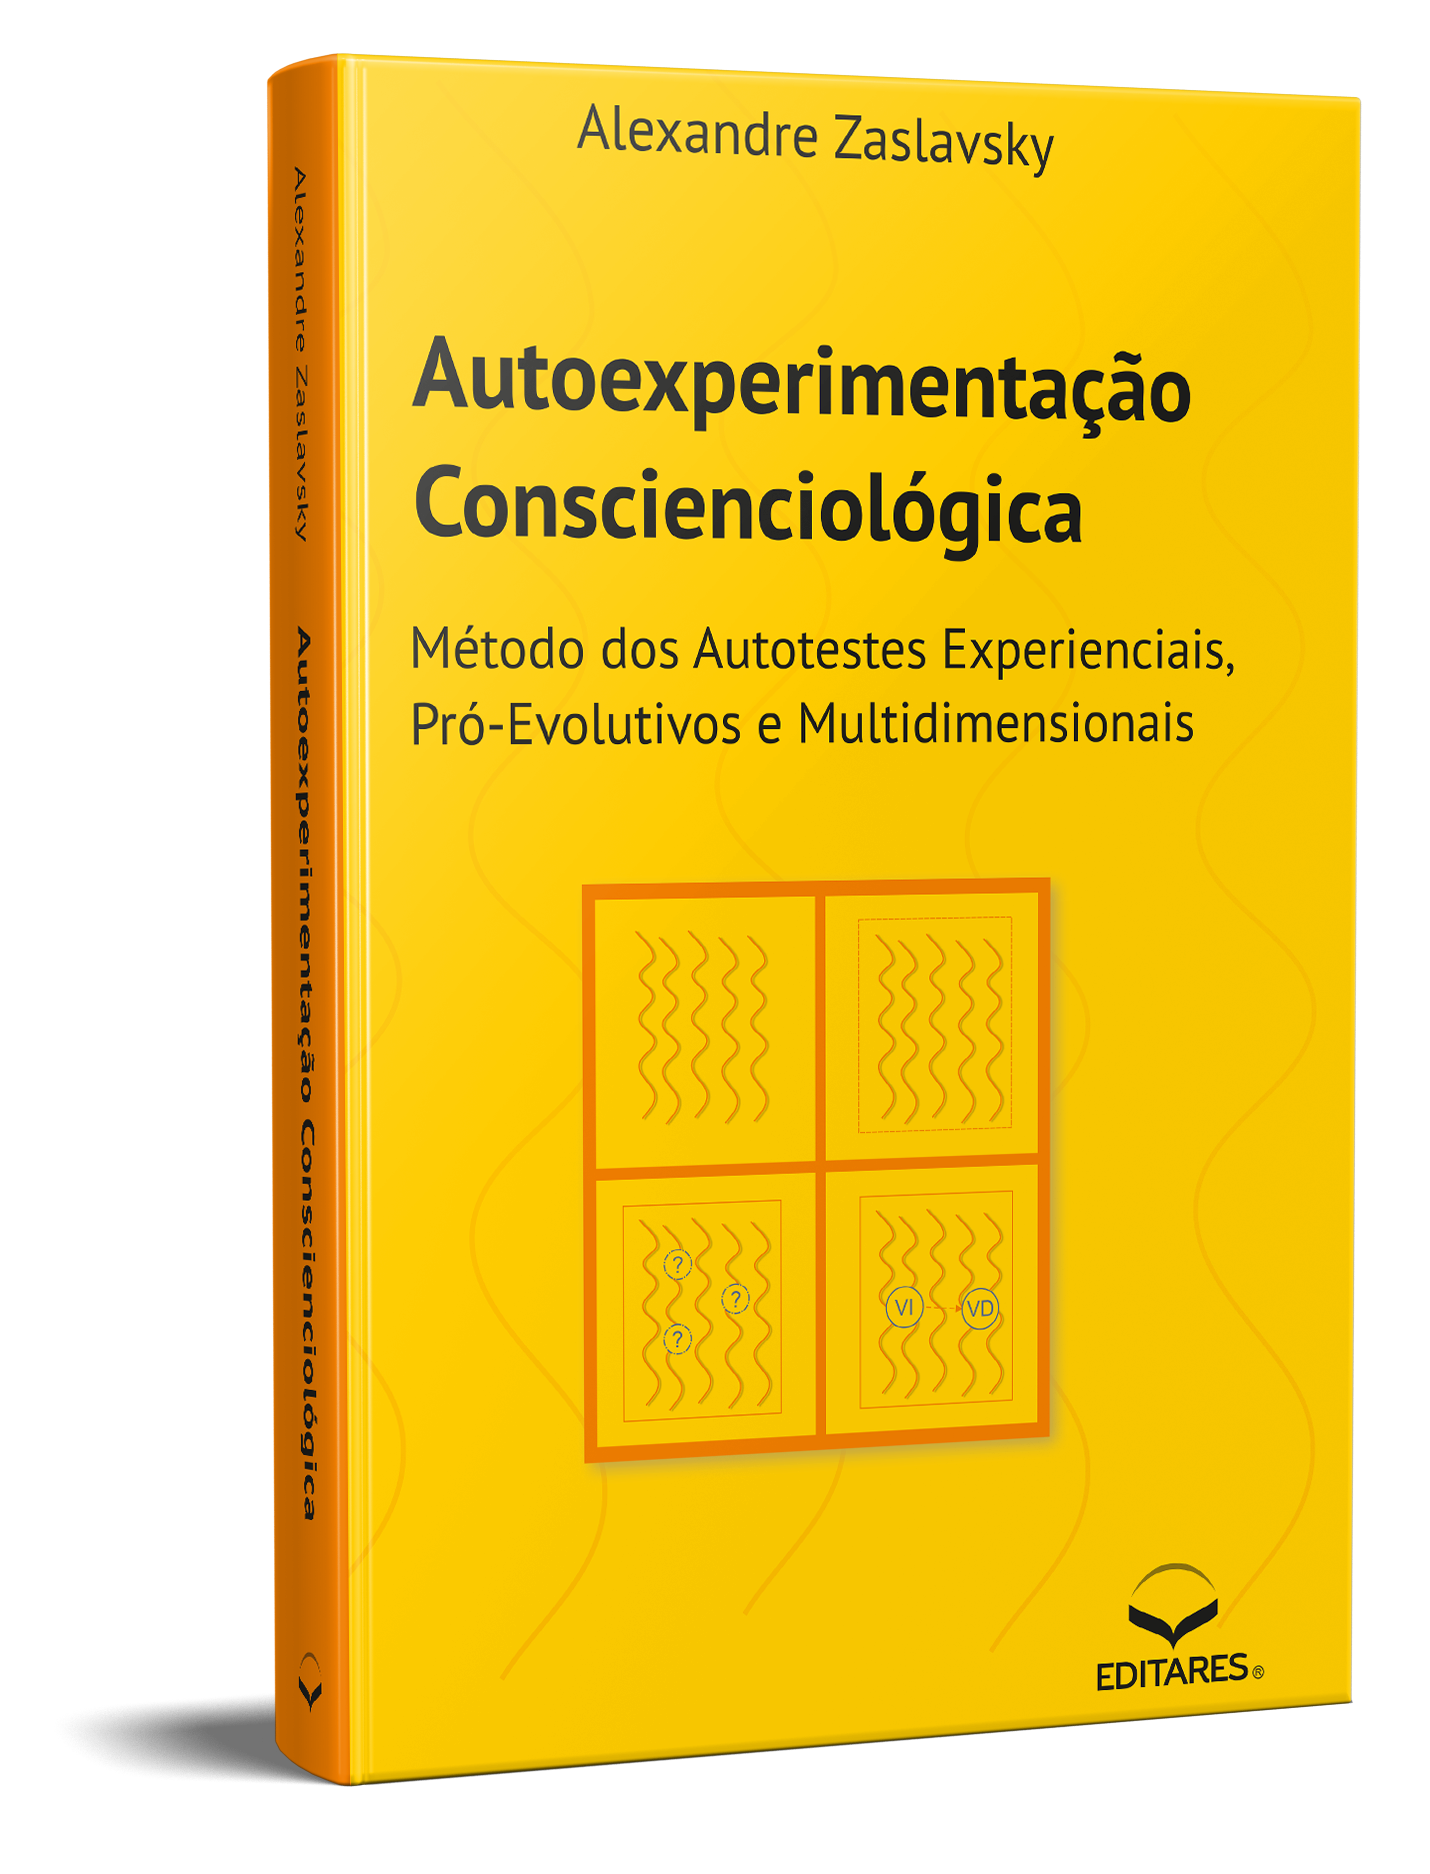
\includegraphics[width=4cm]{articles/entrevista/mockups/Alexandre-Zas.png}
%\end{center}


A Editares é~resultado do \textbf{esforço coletivo de consciências engajadas na tarefa do esclarecimento (tares).} Cada livro, cada publicação e~cada projeto só são possíveis graças à~dedicação dos voluntários que integram nossas equipes. A~seguir, apresentamos a~listagem completa dos atuais voluntários, organizados por áreas de atuação, como forma de reconhecer e~valorizar o~trabalho diário que sustenta o~trabalho editorial da instituição.

\emph{``Voluntariado: autodemonstração interassistencial.''} -- Waldo Vieira.

\begin{longtable}[]{@{}
  >{\raggedright\arraybackslash}p{(\linewidth - 2\tabcolsep) * \real{0.3000}}
  >{\raggedright\arraybackslash}p{(\linewidth - 2\tabcolsep) * \real{0.7000}}@{}}
\toprule\noalign{}
\begin{minipage}[t]{\linewidth}\centering
\textbf{Equipes}
\end{minipage} & \begin{minipage}[t]{\linewidth}\centering
\textbf{Voluntários}
\end{minipage} \\
\hline
\begin{minipage}[t]{\linewidth}\raggedright
Acessibilidade
\end{minipage} & \begin{minipage}[t]{\linewidth}\raggedright
Fabiane Cattai; Lurdes Sousa; Rui Sousa; Sónia Luginger.
\end{minipage} \\
\hline
\begin{minipage}[t]{\linewidth}\raggedright
Biblioteconomia
\end{minipage} & \begin{minipage}[t]{\linewidth}\raggedright
Beatriz Cestari; Betânia Abreu.
\end{minipage} \\
\hline
\begin{minipage}[t]{\linewidth}\raggedright
Comercial
\end{minipage} & \begin{minipage}[t]{\linewidth}\raggedright
Renata Pialarissi; Ricardo Rezende.
\end{minipage} \\
\hline
\begin{minipage}[t]{\linewidth}\raggedright
Conselheiros Editoriais
\end{minipage} & \begin{minipage}[t]{\linewidth}\raggedright
Ana Claudia Prado; Ana Mazzonetto; Cecília Roma; Cristina Bornia; Cristina Ellwanger; José Ricardo Gomes; Leonardo Rodrigues; Liege Trentin; Magda Stapf Amancio; Meracilde Daroit; Patrícia Pialarissi; Roberta Bouchardet.
\end{minipage} \\ \addlinespace[2pt]
\hline
\begin{minipage}[t]{\linewidth}\raggedright
Coordenação
\end{minipage} & \begin{minipage}[t]{\linewidth}\raggedright
Ana Claudia Prado; Magda Stapf Amancio.
\end{minipage} \\
\hline
\begin{minipage}[t]{\linewidth}\raggedright
Diagramação de \emph{e-books}
\end{minipage} & \begin{minipage}[t]{\linewidth}\raggedright
Erik Scardino; Luiz Eduardo Menezes; Márcia Perrusi; Maria Koltum; Rosana~Cardoso.
\end{minipage} \\ \addlinespace[4pt]
\hline
\begin{minipage}[t]{\linewidth}\raggedright
Diagramação de livros
\end{minipage} & \begin{minipage}[t]{\linewidth}\raggedright
Daniel Ronque; Eduardo Santana; João Feliciano; Kátia Ávila; Liliana Ferreira.
\end{minipage} \\
\hline
\begin{minipage}[t]{\linewidth}\raggedright
Diagramação Gráfica de periódicos
\end{minipage} & \begin{minipage}[t]{\linewidth}\raggedright
Ana Claudia Prado; Luciano Melo; Tatiane Mendonça.
\end{minipage} \\
\hline
\begin{minipage}[t]{\linewidth}\raggedright
Editoração Internacional
\end{minipage} & \begin{minipage}[t]{\linewidth}\raggedright
Cecília Roma; Marcos Paiva; Roberta Bouchardet.
\end{minipage} \\
\hline
\begin{minipage}[t]{\linewidth}\raggedright
Financeiro/Administrativo
\end{minipage} & \begin{minipage}[t]{\linewidth}\raggedright
Alex Sarmento; Amanda Vieira.
\end{minipage} \\
\hline
\begin{minipage}[t]{\linewidth}\raggedright
Conselho Fiscal
\end{minipage} & \begin{minipage}[t]{\linewidth}\raggedright
Carlos Moreno; Izabel Conceição; Maria Zilá.
\end{minipage} \\
\hline
\begin{minipage}[t]{\linewidth}\raggedright
\emph{Lives} (transmissões)
\end{minipage} & \begin{minipage}[t]{\linewidth}\raggedright
Blandina Monteiro; Lurdes Sousa; Rui Sousa.
\end{minipage} \\
\hline
\begin{minipage}[t]{\linewidth}\raggedright
Mídias Sociais
\end{minipage} & \begin{minipage}[t]{\linewidth}\raggedright
Paula Gabriella Barbosa; Cassianne Teixeira.
\end{minipage} \\
\hline
\begin{minipage}[t]{\linewidth}\raggedright
Pareceristas
\end{minipage} & \begin{minipage}[t]{\linewidth}\raggedright
Amanda Vieira; Dayane Rossa; João Paulo; Liliana Ferreira; Márcia Perrusi; Rúbia Henning; Conselheiros Editoriais.
\end{minipage} \\ \addlinespace[2pt]
\hline
\begin{minipage}[t]{\linewidth}\raggedright
Revisores de Diagramação e~Prova Final
\end{minipage} & \begin{minipage}[t]{\linewidth}\raggedright
Niciano Vilas Boas.
\end{minipage} \\ \addlinespace[4pt]
\hline
\begin{minipage}[t]{\linewidth}\raggedright
Revisores Linguístico-Textual
\end{minipage} & \begin{minipage}[t]{\linewidth}\raggedright
Bruno Camargo; Liliane Sakakima; Tatiane Mendonça.
\end{minipage} \\
\hline
\begin{minipage}[t]{\linewidth}\raggedright
Soluções Tecnológicas
\end{minipage} & \begin{minipage}[t]{\linewidth}\raggedright
Eduardo Santana.
\end{minipage} \\
\hline
\begin{minipage}[t]{\linewidth}\raggedright
Voluntariado
\end{minipage} & \begin{minipage}[t]{\linewidth}\raggedright
Blandina Monteiro; Magda Stapf Amancio.
\end{minipage} \\
\hline
\begin{minipage}[t]{\linewidth}\raggedright
\emph{Website}
\end{minipage} & \begin{minipage}[t]{\linewidth}\raggedright
Leonardo Ribeiro.
\end{minipage} \\
\midrule\noalign{}
\endhead
\bottomrule\noalign{}
\endlastfoot
\end{longtable}


%\noindent
\includegraphics[width=9cm, height=9cm]{articles/resumo/fotos/materia1/IMG20241023143149.jpg}
        
%    \end{multicols}
\end{document}

    \documentclass{gescons}

\genre {Atualizações}
\author{Roberta Bouchardet e Amanda Vieira}
\authorrole{Coordenadora e Monitora da Escola de Editores}
\title{Nova Escola de Editores Impulsiona Formação Editoriológica na Editares}

\begin{document}
    \makeentrevistatitle
    %\maketitle

    %\fullwidthimage{fields}{b}

    %\coverart{back/editorial}
    \coverart{../fundo-generico.png}
    
    
\begin{center}
    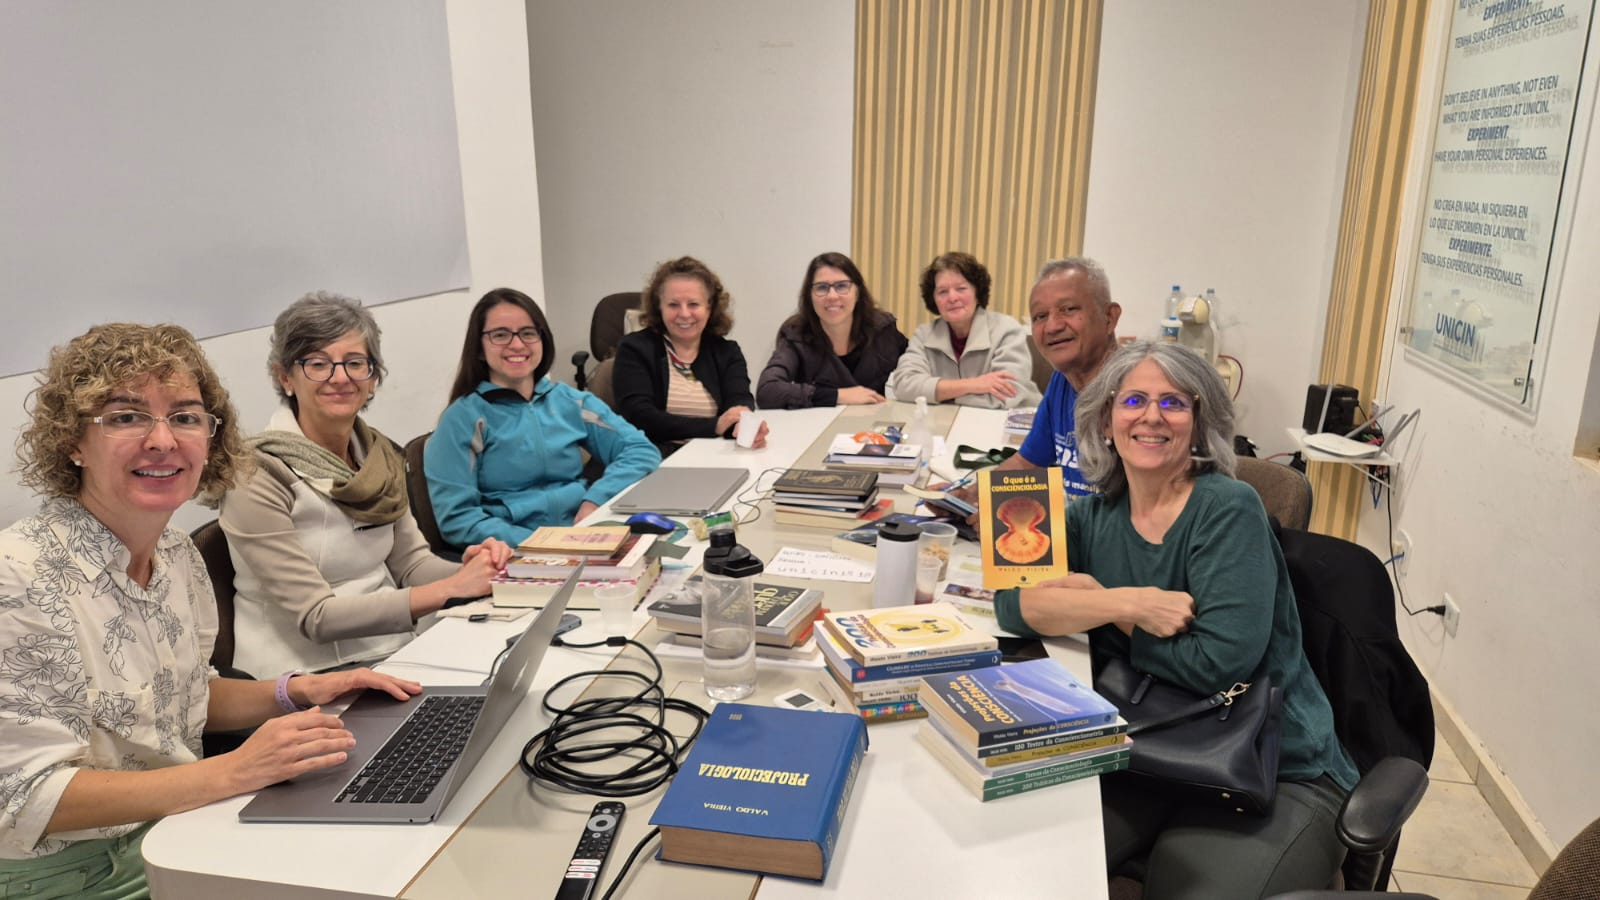
\includegraphics[height=10cm]{articles/atualizacoes/fotos/escola-editores/escola-editores4.jpeg} 
\end{center}
    
    \begin{multicols}{2}

%\section{Nova Escola de Editores impulsiona formação editoriológica na Editares}\label{nova-escola-de-editores-impulsiona-formauxe7uxe3o-editorioluxf3gica-na-editares}

Em julho de 2025, teve início a \emph{Escola de Editores Conscienciológicos.} Trata-se de iniciativa inédita, objetivando formar e qualificar voluntários do \emph{Conselho Editorial.} O curso foi formulado pelos atuais conselheiros, ex-gestores da Editares, voluntários da UNICIN e da CCCI com experiência no processo editorial. \textbf{A meta é ampliar o número de editores, qualificar as publicações, otimizar o fluxo editorial e ampliar a interação entre os editores mais experientes com os novos.}

A \emph{Escola} responde à crescente demanda de autores e livros. A proposta ganhou corpo com apoio da UNICIN, dentro do movimento de reestruturação institucional realizado em 2025. Com 11 módulos quinzenais aos domingos, em formato híbrido, o curso vai até dezembro deste ano, combinando teoria e prática editorial.

A expectativa é consolidar a formação como etapa contínua da atuação editorial na CCCI, atraindo novos voluntários. A turma piloto servirá como base para ajustes e institucionalização futura da Escola, que poderá ter novas edições ou formato gravado.

Estamos empolgados com a expectativa do que pode resultar em termos de mudança de patamar do conselho editorial!


\begin{center}
    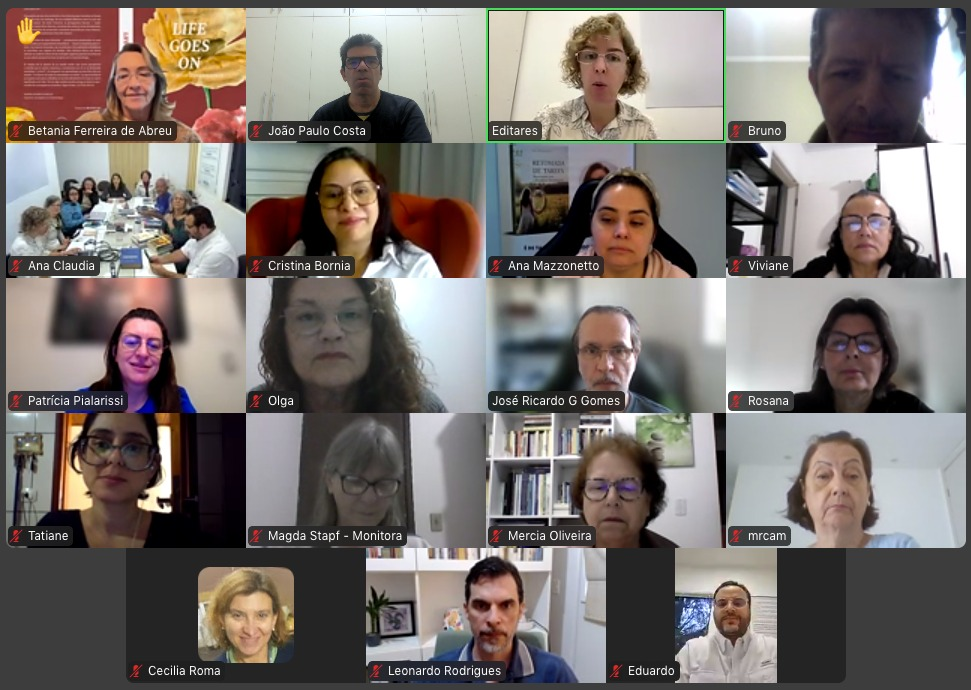
\includegraphics[width=9cm]{articles/atualizacoes/fotos/escola-editores/escola-editores1.jpeg} 
\end{center}


    \end{multicols}
\end{document}

    \documentclass{gescons}

\genre {Atualizações}
\author{Paula Gabriella Barbosa}
\authorrole{Voluntária do Setor de Comunicação da Editares}
\title{Projetos Digitais Modernizam a~Comunicação Editorial da~Editares}
%\roles{Voluntária do Setor de Comunicação da Editares}

\begin{document}
    \makeentrevistatitle
    %\maketitle

    %\fullwidthimage{fields}{b}

    %\coverart{back/editorial}
    \coverart{../fundo-generico.png}
    
    
\begin{center}
    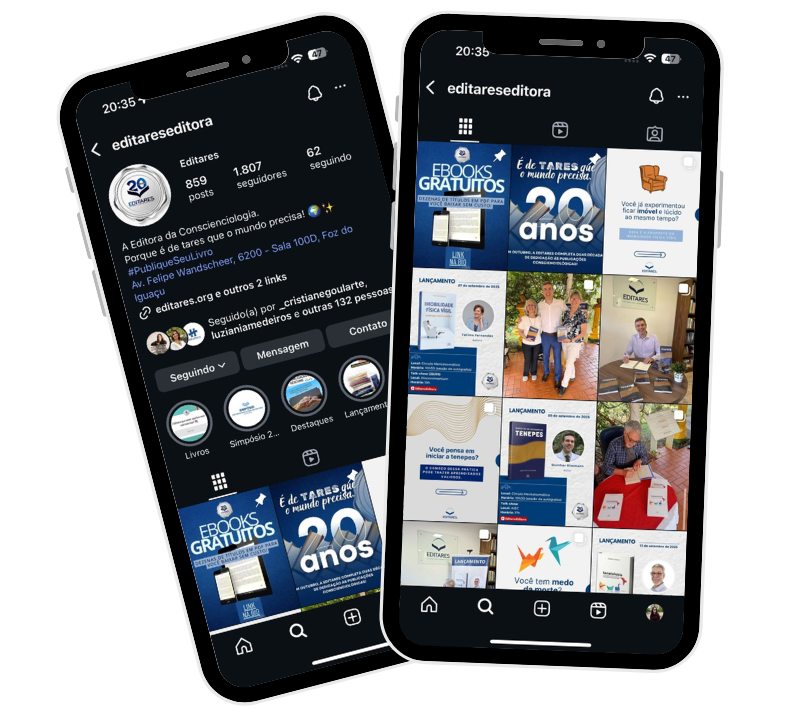
\includegraphics[height=10cm]{articles/atualizacoes/fotos/materia5/Instagram-Editares.png} 
\end{center}
    
    \begin{multicols}{2}


Nos últimos anos, a~comunicação da Editares passou por importantes atualizações. O~trabalho de divulgação não se restringe apenas ao anúncio de novos lançamentos, mas se dedica principalmente a~valorizar e~compartilhar os conteúdos de gescons publicadas. A~proposta é~\textbf{oferecer ao futuro leitor amostra prática} do que encontrará nas obras, ampliando o~alcance de cada livro.

Nesse sentido, a~Editares tem investido em diferentes formatos para tornar o~conteúdo mais acessível e~interativo. Entre eles, destacam-se os vídeos gravados pelos autores, que aproximam o~leitor da vivência pessoal de quem escreveu a~obra, e~os carrosséis produzidos a~partir das resenhas, que apresentam as ideias centrais de maneira visual e~objetiva. Assim, cada publicação nas redes sociais se torna uma oportunidade para aprofundar a~compreensão e~estimular o~interesse pela leitura.

Além disso, a~Editares tem promovido \textbf{ações que fortalecem o~vínculo entre os livros e~a~comunidade conscienciológica.} Dentre elas, destacam-se:

\begin{enumerate}
\def\labelenumi{\arabic{enumi}.}
\item
  Dicas de leitura associadas a~cursos em andamento, criando conexões pertinentes para o~aluno e~favorecem a~interação com as instituições parceiras.
\item
  Campanhas promocionais em datas especiais, como a~promoção do livro Comunicação Evolutiva durante o~aniversário de 20 anos da Comunicons.
\end{enumerate}

Essas iniciativas têm tornado a~Editares mais presente e~ampliado o~alcance do conteúdo das gescons a~um público cada vez maior. Ao divulgar trechos, ideias e~reflexões dos livros, a~Editares reforça seu papel como ponte entre o~conhecimento conscienciológico e~o~leitor, promovendo a~expansão da interassistência por meio da leitura.


% {[}INSERIR FOTO QUE ESTÁ NA PASTA MATÉRIA 5{]}


%\begin{center}
%    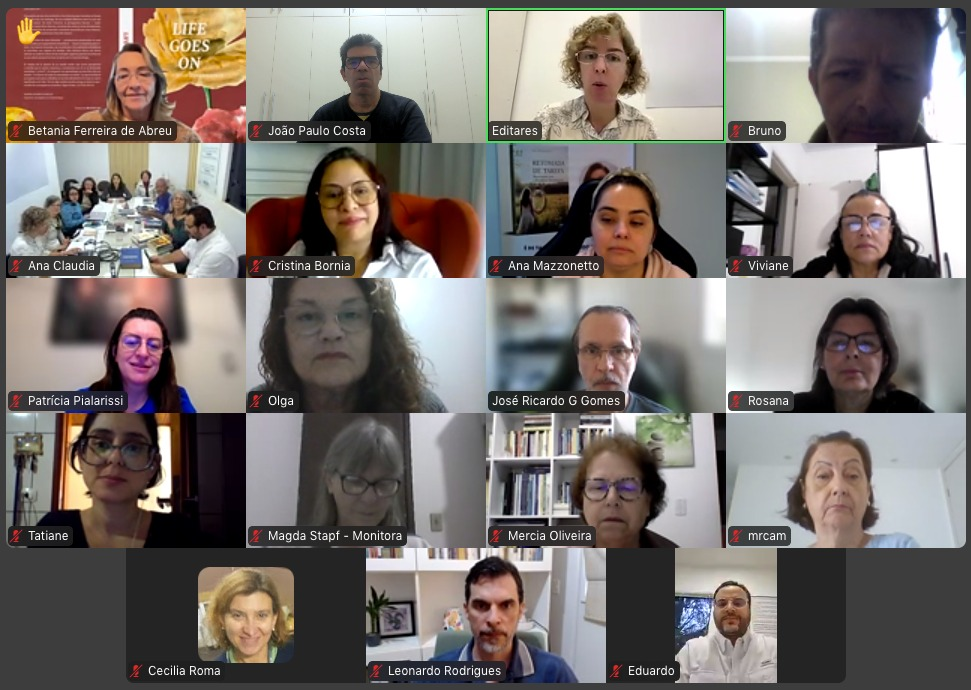
\includegraphics[width=9cm]{articles/atualizacoes/fotos/escola-editores/escola-editores1.jpeg} 
%\end{center}


    \end{multicols}
\end{document}


    \documentclass{gescons}

\genre {Atualizações}
\author{Ana Claudia Prado e Ana Mazzonetto}
\title{Editares lança revista científica especializada em Editoriologia e Publicaciologia}

\begin{document}
    \makeentrevistatitle
    %\maketitle

    %\fullwidthimage{fields}{b}

    %\coverart{back/editorial}
    \coverart{../fundo-generico.png}
    
    
\begin{center}
    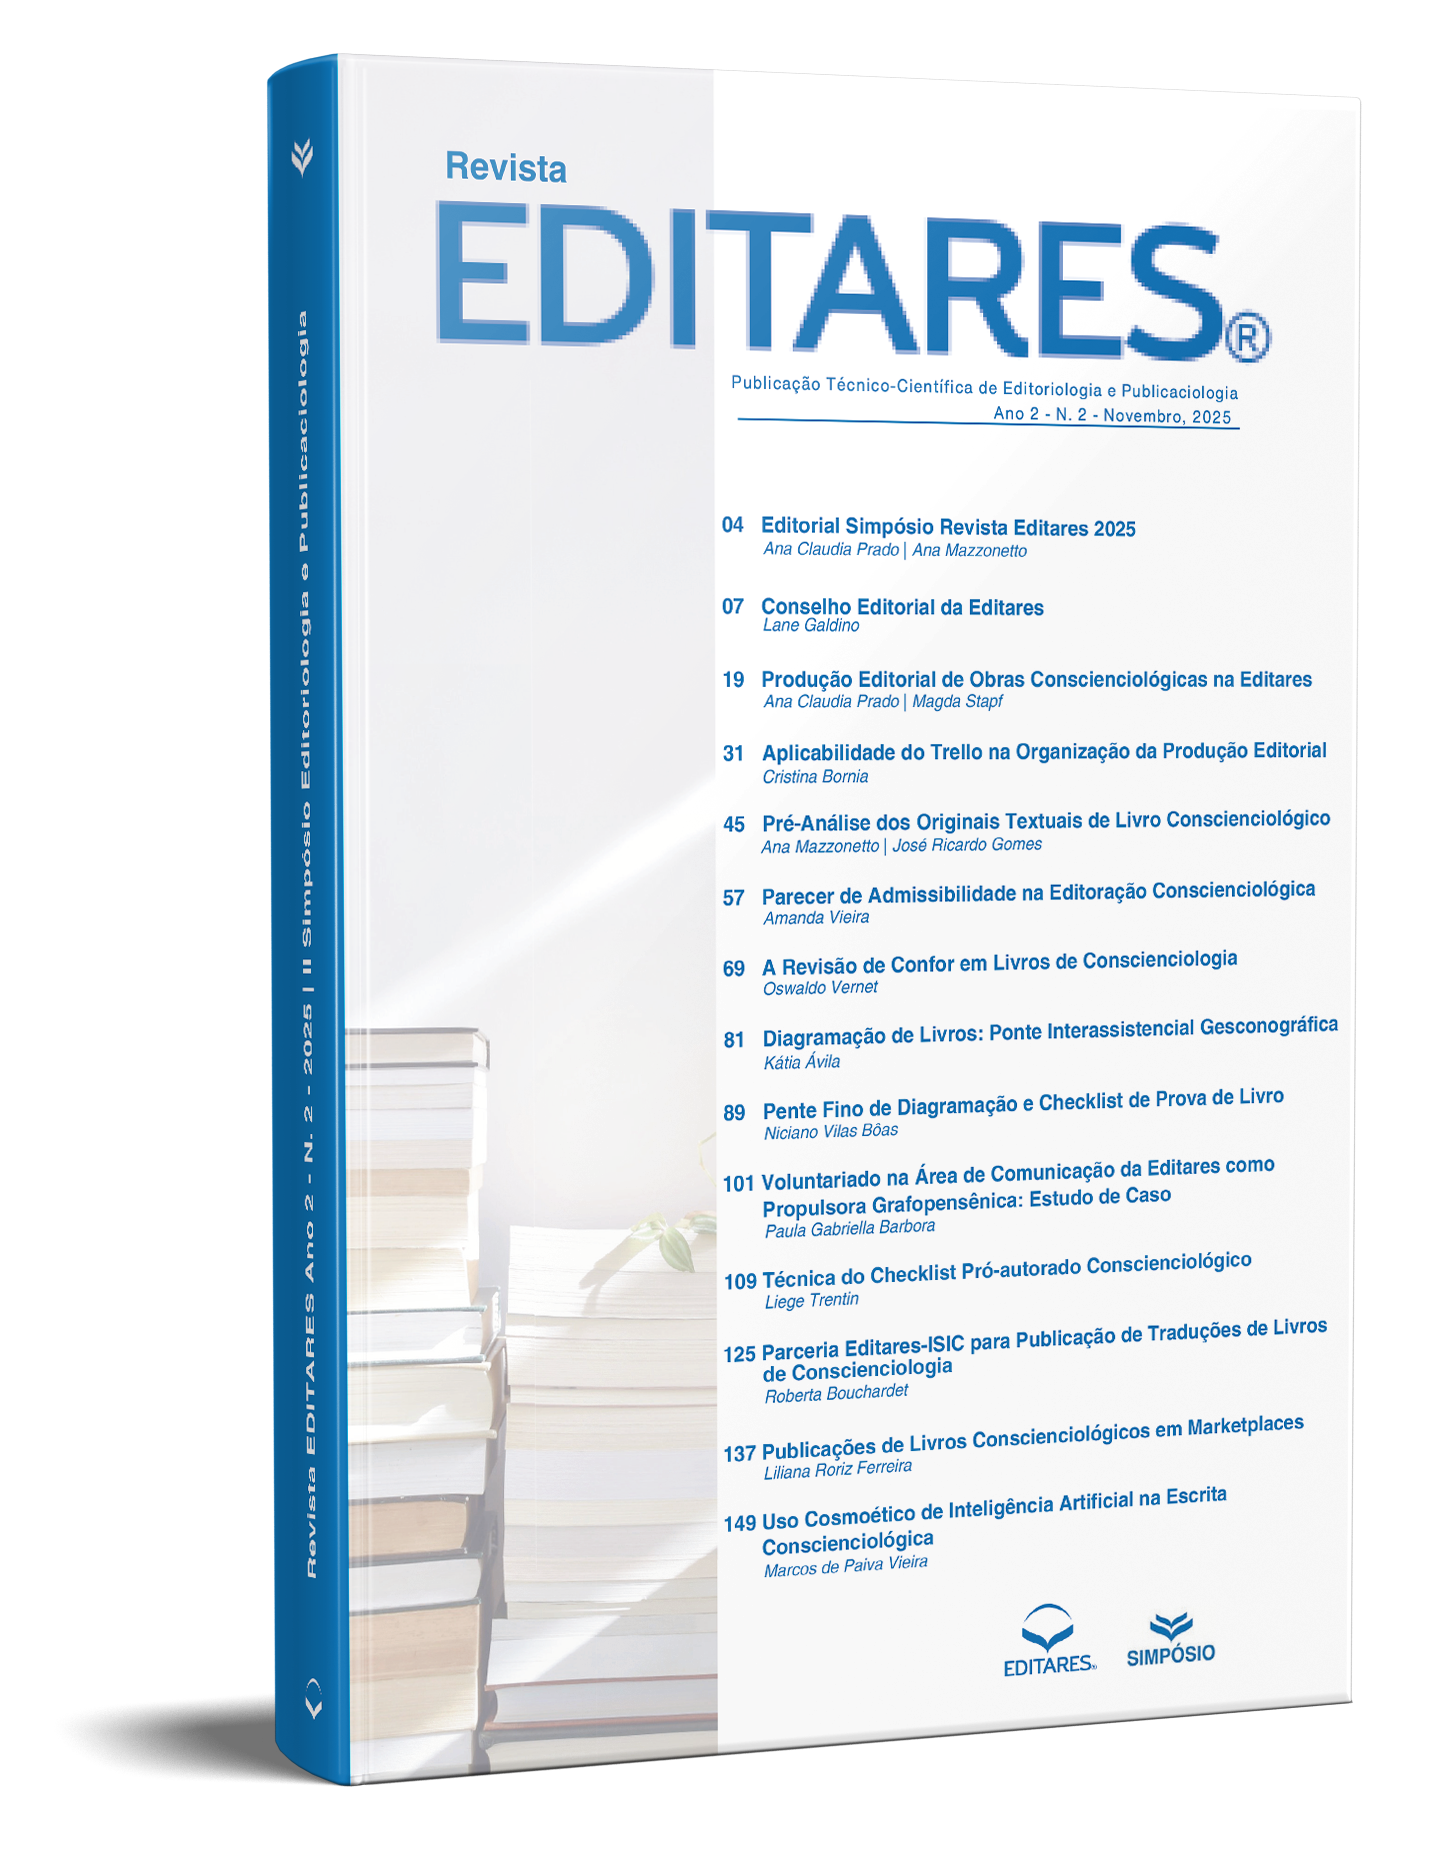
\includegraphics[height=10cm]{articles/atualizacoes/fotos/materia6/revista_editares_2025.png} 
\end{center}
    
    \begin{multicols}{2}


A Associação Internacional Editares dedicada à editoração e publicação de gestações conscienciais, anunciou em novembro de 2025 o lançamento da \textbf{Revista Editares,} publicação científica voltada exclusivamente às especialidades de \emph{Editoriologia e Publicaciologia.} O lançamento ocorreu durante evento temático sobre essas áreas de estudo: \textbf{II Simpósio Editoriologia e Publicaciologia.}

A novidade representa um avanço em relação à edição especial da \emph{Revista Gescons} nº 5, publicada em 2023, quando voluntários da Editares apresentaram, por meio de artigos científicos, os bastidores da produção editorial conscienciológica.

A escolha de um novo nome não se restringe a uma mudança formal. A decisão editorial visa demarcar, de modo preciso, o \textbf{caráter científico da publicação} e a construção de novos conhecimentos a partir de artigos técnicos nas duas especialidades.

Com a criação da \emph{Revista Editares,} a instituição passa a separar claramente os campos de atuação: enquanto a nova publicação concentra análises científicas, a \emph{Revista Gescons} continua sendo o espaço para registro de lançamentos de livros e outras pontuações editoriais e administrativas.

A iniciativa reforça o compromisso da Editares com o profissionalismo editorial, legitima processos de revisão mais exigentes de revisão por pares, fortalece a especialização temática e consolida a identidade científica da instituição.

O primeiro número da \emph{Revista Editares} reúne \textbf{treze artigos inéditos,} abordando desde os meandros do fluxo editorial até as vivências de voluntários no processo de editoração e publicação de obras conscienciológicas, sempre à luz do Paradigma Consciencial.

\emph{``Este é um momento de atualização do processo editorial da Editares, no qual reafirmamos publicamente nosso compromisso com a produção científica nas especialidades de Editoriologia e Publicaciologia''}, ressaltam as editoras Ana Claudia Prado e Ana Mazzonetto.



%\emph{Editoras da Revista Editares}

%\emph{{[}Foto das autoras{]}}

%\emph{{[}INSERIR MOCKUP DA REVISTA QUE ESTÁ NA PASTA MATÉRIA 6{]}}


%\begin{center}
%    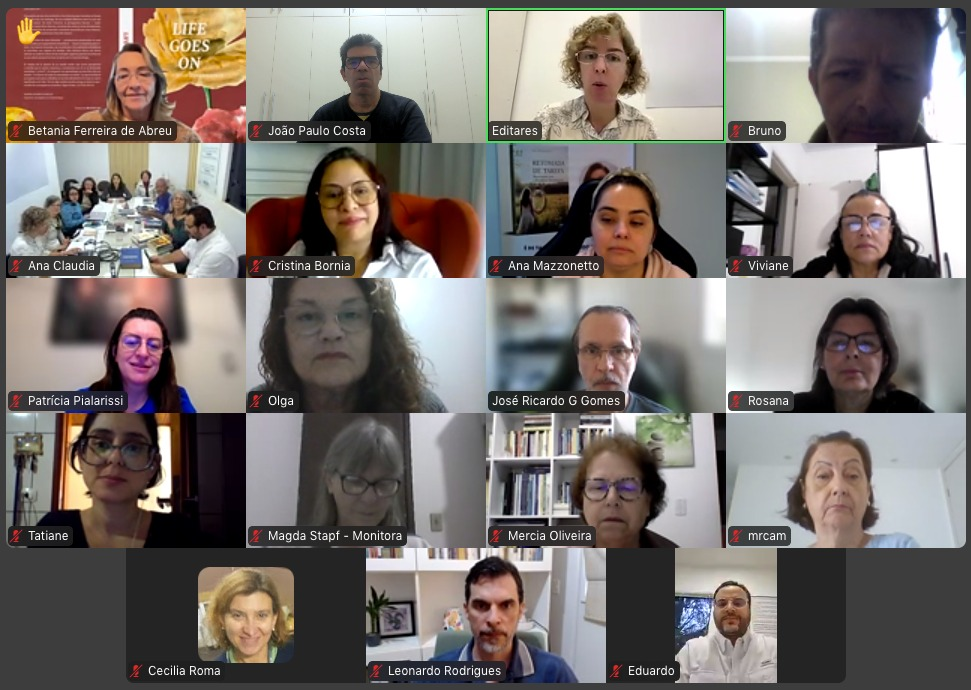
\includegraphics[width=9cm]{articles/atualizacoes/fotos/escola-editores/escola-editores1.jpeg} 
%\end{center}


    \end{multicols}
\end{document}

    
    \genre{}
    \title {Parcerias}
    \author{}
    \authorrole{}
    \makecovertitle{articles/parceria/capa-parceria.png}{}
    
    \documentclass{gescons}

\genre {Parceria}
\author{Ricardo Rezende}
\authorrole{Voluntário do Setor Comercial da Editares}
\title{Editares e IIPC Retomam Parceria para Ampliar a Venda de Livros}

\begin{document}
    \makeentrevistatitle
    %\maketitle

    %\fullwidthimage{fields}{b}

    \coverart{articles/parceria/fundo-parceria.png}
    
    

\begin{center}
    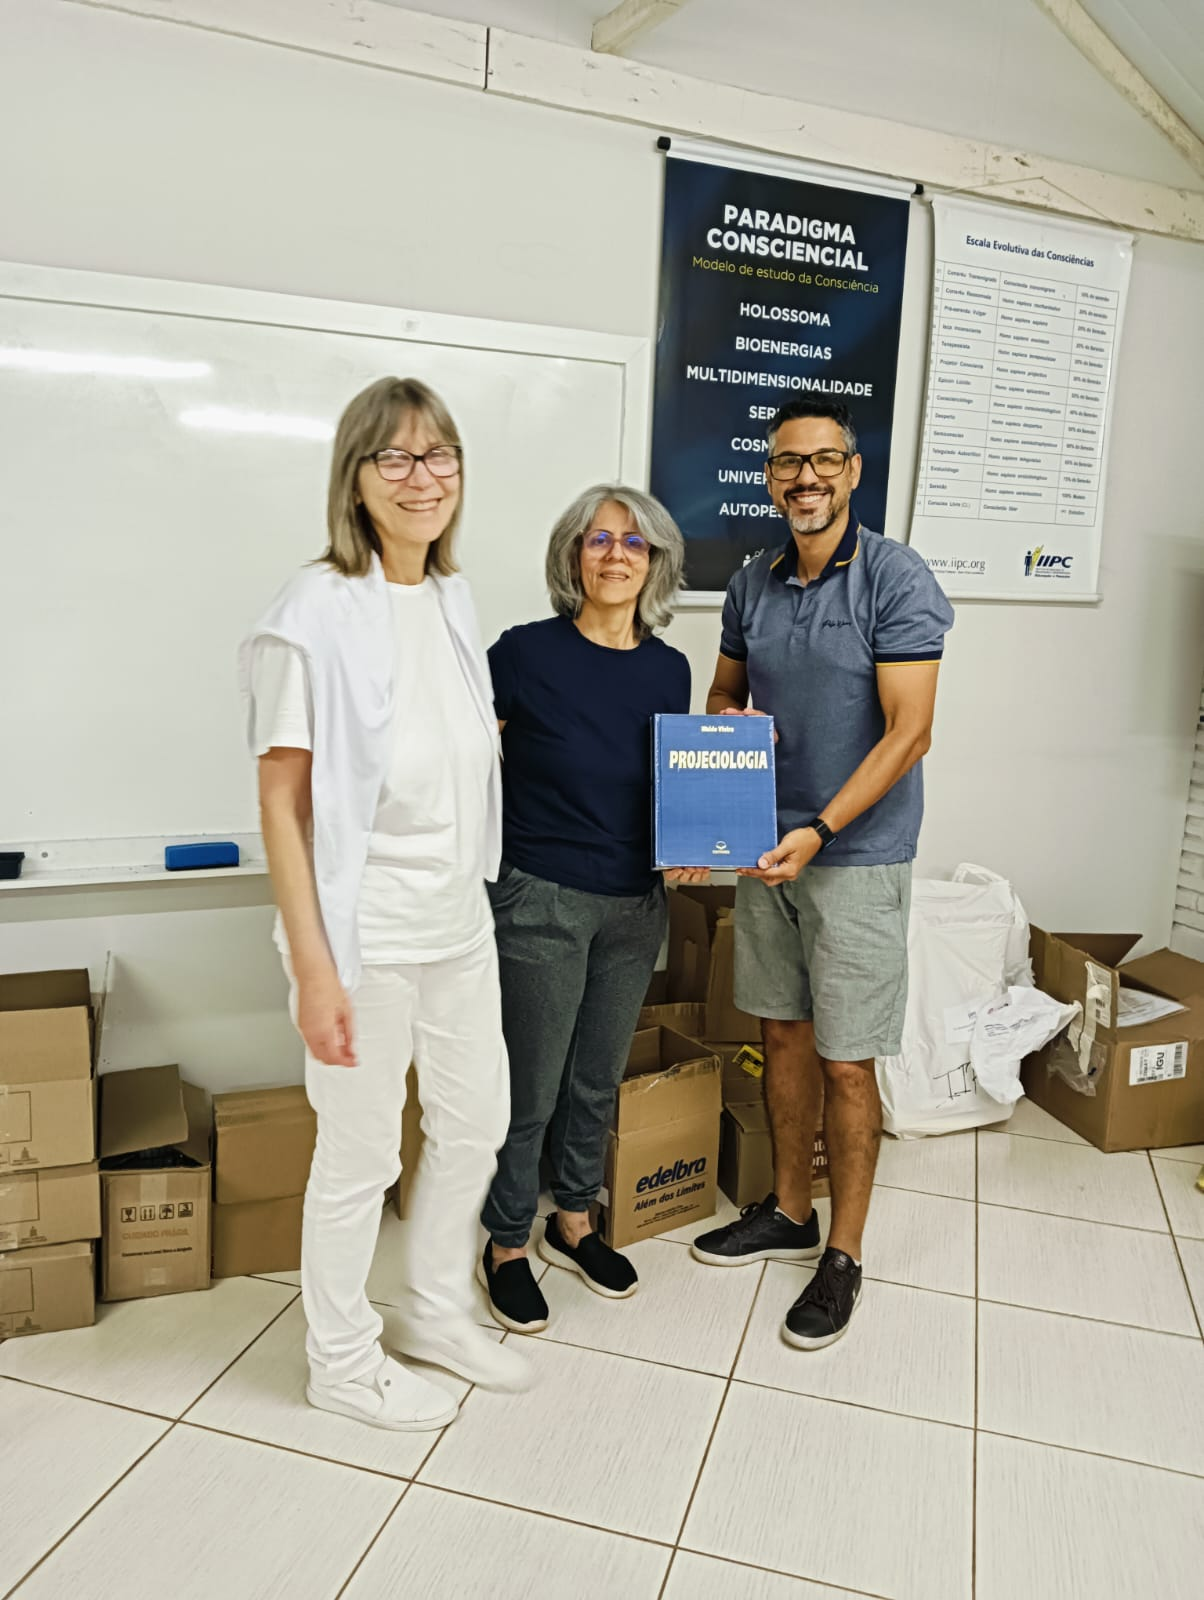
\includegraphics[height=8cm,trim={130 200 100 300},clip]{articles/parceria/imagens/editares-iipc.jpeg}
\end{center}


    
%    \begin{multicols}{2}


%\begin{wrapfigure}[11]{o}{0.5\textwidth}
%  %\begin{left}
%  %\vspace{-15mm}
%  %\hspace{1mm}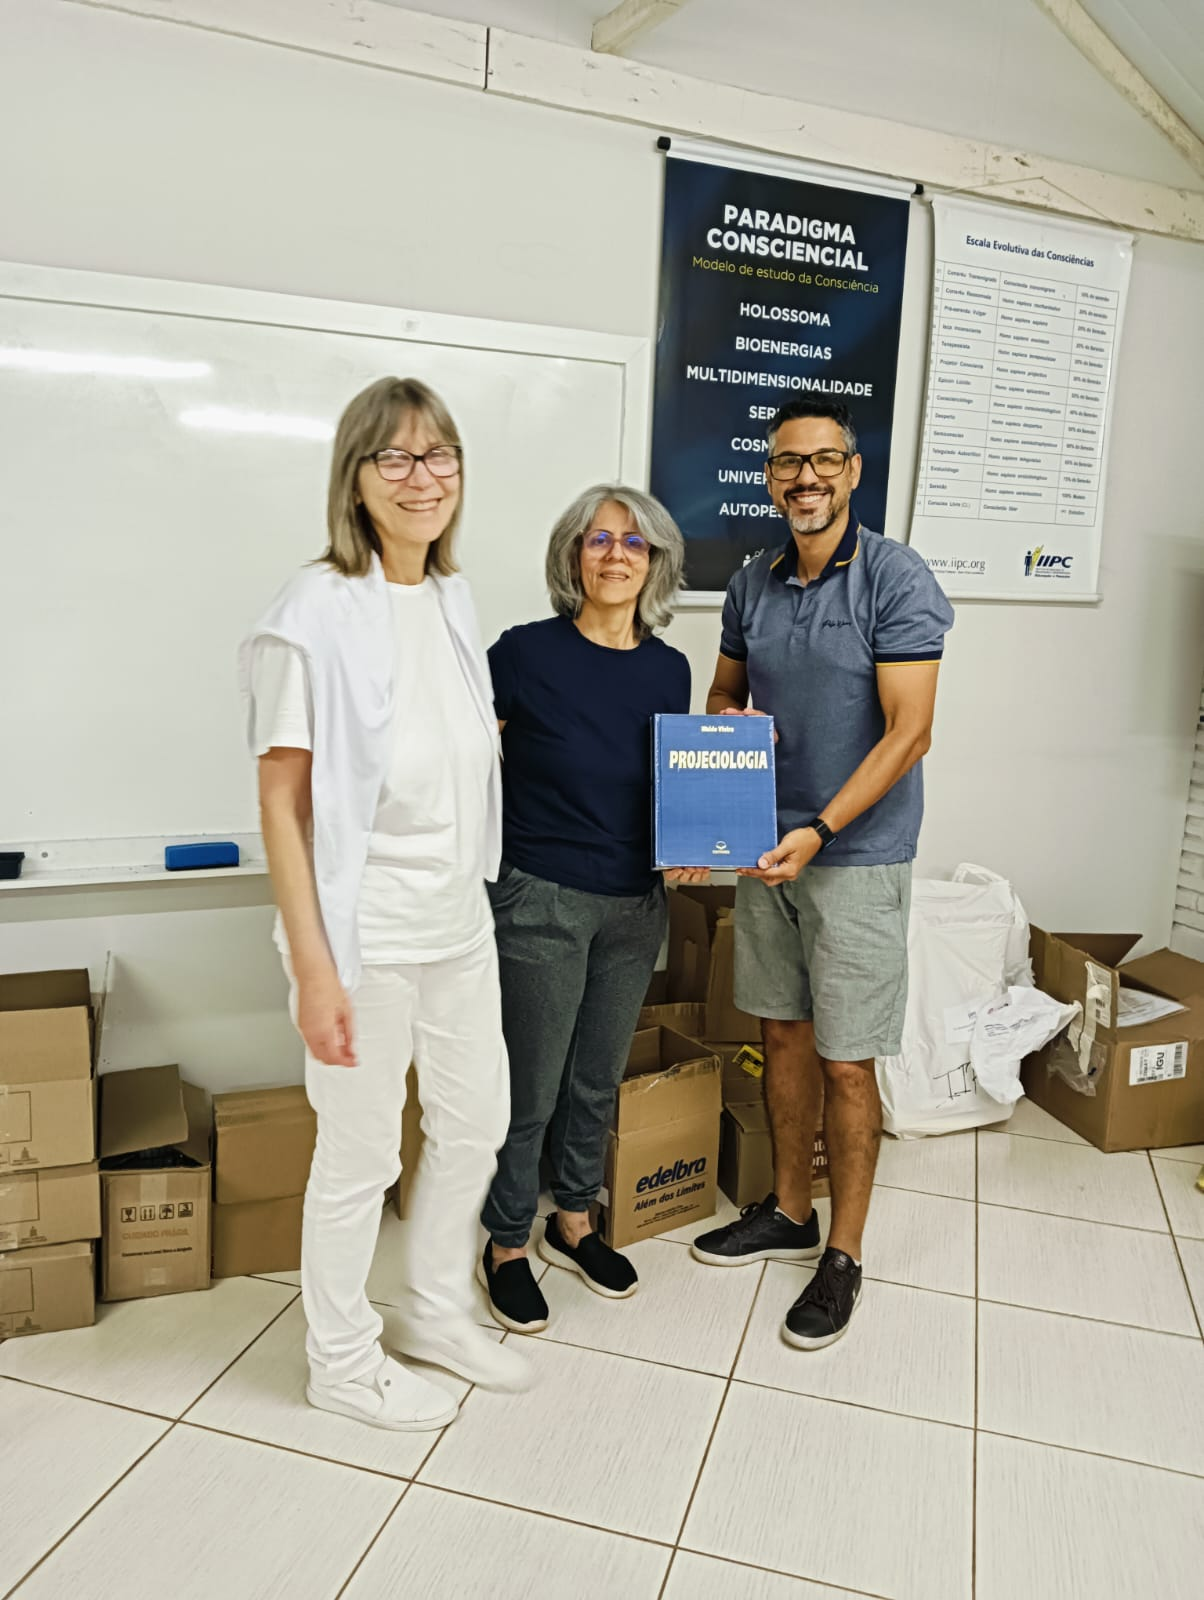
\includegraphics[height=10cm]{articles/parceria/imagens/editares-iipc.jpeg}
%  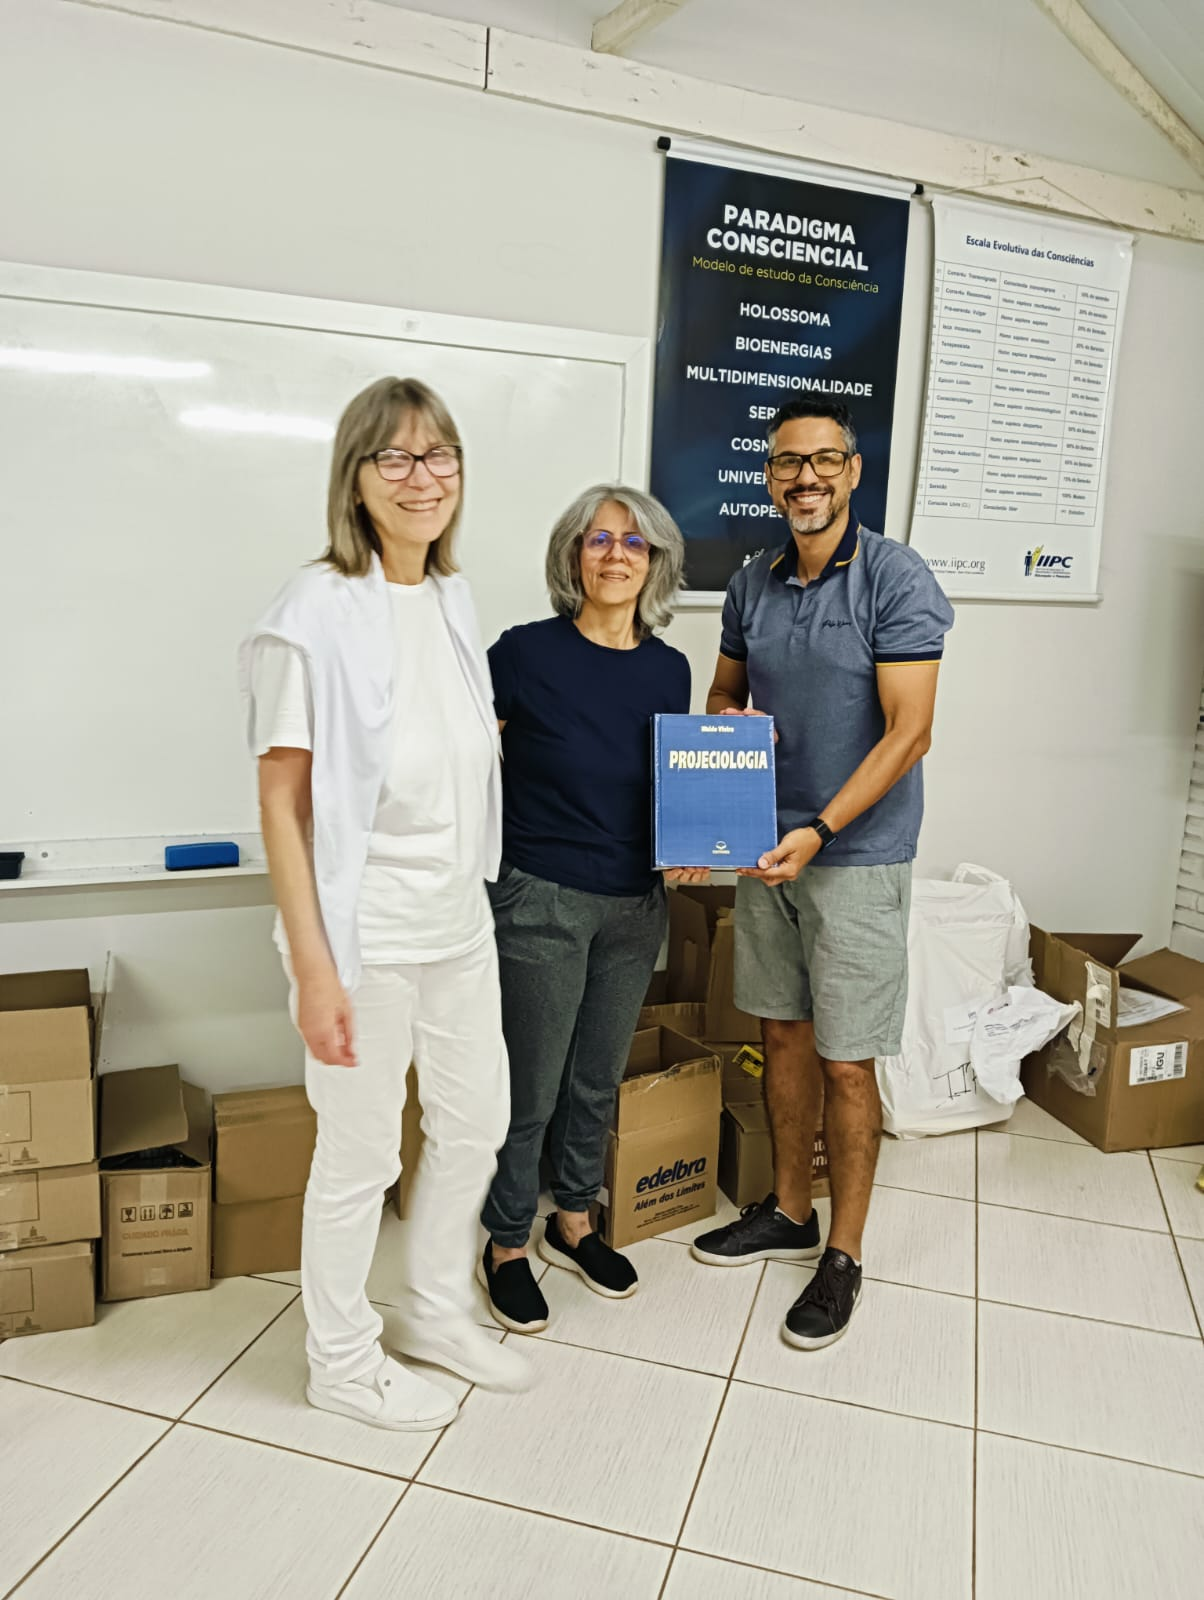
\includegraphics[height=8cm,trim={130 200 100 300},clip]{articles/parceria/imagens/editares-iipc.jpeg}
%  %\end{left}
%\end{wrapfigure}

\vspace{5mm}

Neste ano, a Editares, coordenada pelas voluntárias Ana Claudia Prado e Magda Stapf Amancio, celebra acordo exitoso com a coordenação geral e equipe do IIPC, representados pelos coordenadores gerais Gabriel Araújo e Ailton Maia, pelo qual \textbf{as obras conscienciológicas} estão sendo disponibilizadas para compra nos acervos dos \emph{Centros Educacionais de Autopesquisa} (CEAs) do \emph{Instituto Internacional de Projeciologia e Cons­cienciologia} (IIPC).

A renovação dessa parceria, além de possibilitar a melhoria logística da distri­buição comercial desses livros, auxiliará na ampliação da difusão tarística dos livros pu­blicados por autores conscienciológicos, ao permitir o acesso físico às gestações conscien­ciais para os visitantes e voluntários nos CEAs do IIPC.

\vspace{5mm}

\begin{center}
    
\includegraphics[height=4cm]{images/Logo-Editares-com-Marca-Registrada.png}
    \hspace{3cm}
    
\includegraphics[height=4cm]{images/IIPC_logo.png} 
\end{center}


% \begin{quote}
% \emph{Por: Ricardo Rezende}
% \emph{Voluntário do Setor Comercial da Editares}
% \emph{{[}FOTO DO AUTOR{]}}
% \end{quote}



%\emph{Editoras da Revista Editares}

%\emph{{[}Foto das autoras{]}}

%\emph{{[}INSERIR MOCKUP DA REVISTA QUE ESTÁ NA PASTA MATÉRIA 6{]}}


%\begin{center}
%    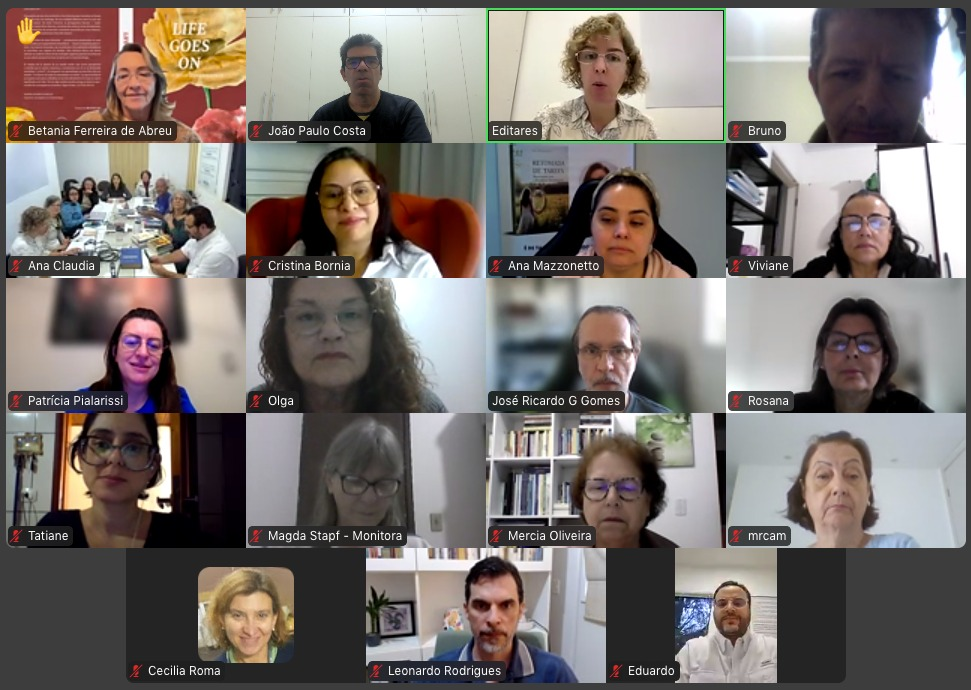
\includegraphics[width=9cm]{articles/atualizacoes/fotos/escola-editores/escola-editores1.jpeg} 
%\end{center}


%    \end{multicols}
\end{document}

    \documentclass{gescons}

\genre {Parceria}
\author{Ana Claudia do Prado e~Magda Stapf Amancio}
\authorrole{Coordenadoras Gerais da Editares}
\title{Editares e~Uniescon Firmam Acordo Inédito de Cooperação Interinstitucional}

\begin{document}
    \makeentrevistatitle
    %\maketitle

    %\fullwidthimage{fields}{b}

    %\coverart{back/editorial}
    \coverart{articles/parceria/fundo-parceria.png}
    
    
\begin{center}
    
\includegraphics[height=4cm]{images/Logo-Editares-com-Marca-Registrada.png}
    \hspace{3cm}
    
\includegraphics[height=5cm]{images/Logo-UNIESCON-2048x1741.png} 
    
    %\includegraphics[height=10cm]{articles/parceria/imagens/parceria-editares-uniescon.png}
    %\includegraphics[height=10cm]{example-image}
\end{center}
    
    \begin{multicols}{2}

A produção conscienciológica ganha um novo impulso. Em julho de 2025, a~Editares e~a~Uniescon firmaram um \textbf{acordo inédito de cooperação interinstitucional.} O~objetivo é~compartilhar os pareceres gesconográficos de autorandos, contribuindo para a~qualificação de obras em fase de construção e~revisão, de acordo com os trâmites editoriais das duas instituições.

O intercâmbio dos pareceres será realizado somente mediante consentimento prévio e~expresso do autorando, garantindo transparência e~respeito ao processo autoral. Editares e~Uniescon também assumiram o~compromisso de \textbf{preservar a~confidencialidade dos arquivos} e~manter sigilo sobre o~material que estiver fora do fluxo autorizado.

Com a~iniciativa, Editares e~Uniescon \emph{consolidam um trabalho conjunto em prol da melhoria contínua da produção da gesconografia conscienciológica,} criando novas pontes de apoio para pesquisadores e~escritores.



    \end{multicols}
\end{document}

    \documentclass{gescons}

\genre {Parceria}
\author{Amanda Vieira}
\authorrole{Voluntária da Editares}
\title{Grupos de Trabalho com a~UNICIN Traçam Planos para Fortalecer a~Atuação da Editares}

\begin{document}
    \makeentrevistatitle
    %\maketitle

    %\fullwidthimage{fields}{b}

    %\coverart{back/editorial}
    \coverart{articles/parceria/fundo-parceria.png}

\begin{center}
    \hspace{0.5cm}
    
\includegraphics[height=3cm]{images/Logo-Editares-com-Marca-Registrada.png}
    \hspace{3cm}
    
\includegraphics[height=2cm]{images/Unicin-Logo-1024x315.png} 
\end{center}

    
    \begin{multicols}{2}



Em 2025, a~Editares deu importante passo estratégico para potencializar sua atuação na produção e~distribuição de gescons. Em parceria com a~UNICIN e~a~UNIESCON, foram criados \textbf{dois grupos de trabalho (GTs)} voltados à~reformulação de processos e~à~implantação de novas iniciativas, com foco em dois pontos principais: o~fluxo editorial e~a~venda de livros.

Os encontros reuniram voluntários de diferentes ICs e~áreas de atuação, evidenciando a~importância da intercooperação na Comunidade Conscienciológica. Dessa troca nasceram dois GTs específicos: GT Editorial e~GT Comercial.

\subsection*{Diagnóstico, planejamento e~ação}

Durante o~primeiro semestre, os subgrupos trabalharam em diagnósticos detalhados, mapeando gargalos, levantando necessidades e~propondo soluções. A~partir desse estudo, foram elaborados planos de ação que começaram a~ser implementados no segundo semestre de 2025.

No \textbf{GT Comercial,} as iniciativas se voltaram à~expansão da presença da Editares, com novos processos de \emph{marketing}, estratégias de divulgação e~ações de lançamento de livros. 

No \textbf{GT Editorial,} o~destaque foi a~criação da \emph{Escola de Editores,} um projeto voltado à~capacitação de voluntários para ampliar a~qualidade técnica e~a~celeridade na editoração de obras conscienciológicas.

\subsection*{A força do voluntariado e~a~união das ICs}

O movimento reforça a~relevância da união entre as Instituições Conscienciocêntricas como fator-chave para a~expansão da Conscienciologia. A~intercooperação entre Editares, UNICIN e~UNIESCON potencializa a~produção e~a~difusão das gescons, beneficiando pesquisadores, autores e~leitores.

Nesse contexto, o~voluntariado se destaca como força motriz da \emph{reurbanização extrafísica} (reurbex), atuando na materialização de projetos que impactam diretamente a~evolução grupal. O~livro, enquanto ferramenta de autopesquisa e~recomposição grupocármica, cumpre papel central no esclarecimento e~na ampliação da lucidez planetária.

Com essas iniciativas, a~Editares reafirma seu compromisso com a~qualidade editorial, a~celeridade dos processos e~a~ampliação da distribuição das obras conscienciológicas. Mais do que uma reorganização interna, trata-se de um movimento coletivo que coloca o~livro e~o~conhecimento técnico ao serviço da evolução pessoal e~grupal.





    \end{multicols}
\end{document}

    
    \genre{}
    \title {Entrevistas com os autores}
    \author{}
    \authorrole{}
    \makecovertitle{articles/entrevista/fundo-entrevistas.png}{}

    \documentclass{gescons}

\genre {Entrevista}
\author{Daniel Mamede}
\title{Ações Antifanatismo: Intensidade Lúcida em Autopesquisas e Autorreciclagens}

\begin{document}
    \makeentrevistatitle

    \coverart{back/Daniel-Mamede}
    \begin{multicols}{2}

\begin{center}
    
\includegraphics[width=8cm]{articles/entrevista/mockups/Daniel-Mamede.png}
\end{center}

%\noindent\includegraphics[width=9cm, height=10cm]{example-image} 

\textbf{1. Qual foi a motivação para a escrita da obra? Por que a definição deste tema para publicação de um livro?}

O livro “Ações Antifanatismo” representa muito para mim, por ter sido o resumo dos meus 10 primeiros anos de contato e vivência do paradigma consciencial. 

Escrito em princípio para mim mesmo, para poder organizar, reeducar e curar aspectos negativos das automanifestações, muitas delas tendentes ou vinculadas ao fanatismo, o livro mostrou \textit{a vida teática no papel,} isto é, materializou, grafou e vincou a autopesquisa conscienciológica sendo vivenciada dia a dia, pensene a pensene, aprendizado a aprendizado, resultando em material com enorme potencial para ajudar outras pessoas que possam estar em apuros com o mesmo assunto, notadamente os intermissivistas, os quais partilham de propósitos e objetivos similares aos meus para esta vida humana.



\textbf{2. Quais foram as principais percepções, intra e extrafísicas, durante a pesquisa e a escrita da obra? E posterior ao lançamento?}

O que este livro mais tem são percepções e parapercepções vivenciadas durante os processos de reciclagem, pois seu estilo de escrita predominante foi o do “\textit{in media res}”, isto é, as experiências da vida eram grafadas e autocriticadas de modo praticamente concomitante às ocorrências. Vale muito a pena conferir. 


\textbf{3.       Qual o maior aprendizado com a escrita desta obra?}

Nos últimos 10 anos, nunca deixei passar mais que 24 horas entre o intervalo da ocorrência dos fatos ou parafatos e as devidas anotações. Por isso, o efeito das vivências descritas no livro traz as energias dos momentos das aprendizagens disruptivas de modo bastante intenso e real. E essa rotina continua firme na minha vida, mesmo após a conclusão do livro, pois a autopesquisa conscienciológica nunca pode parar. Este foi meu maior aprendizado ao ver o livro concluído.

\begin{pullquote}
``O efeito das vivências descritas no livro traz as energias dos momentos das aprendizagens disruptivas de modo bastante intenso e real.''
\end{pullquote}


\textbf{4.       O que poderiam dizer como incentivo para que mais pesquisadores invistam na publicação de obras conscienciológicas?}

Fazer autopesquisas diárias e comprometidas como as descritas em “Ações Antifanatismo” é um dos caminhos mais tranquilos para quem quiser publicar algum livro. Ele vai acontecer naturalmente. Vai estar pronto antes mesmo de o autor o conceber. Foi assim comigo. O acúmulo dos pensenes materializados no papel gerou banco de dados rico e vasto para eu poder explorá-lo da maneira que entendesse por bem, e assim o fiz justamente para trabalhar os traços de temperamento que entendi serem os mais sérios e prioritários em meus processos de reciclagem, no caso, vinculados às posturas fanáticas. Aí, foi só organizar. A rigor, o que direcionou e conduziu a escrita do livro não foi a atenção ao traf\textit{a}r do fanatismo, mas sim ao traf\textit{o}r da valorização e do comprometimento com a ininterruptibilidade da autopesquisa conscienciológica.


    
    
    \end{multicols}
\end{document}
                       % Ações Antifanatismo
    \documentclass{gescons}

\genre {Entrevista}
\author{Alexandre Zaslavksy}
\title{Autoexperimentação Conscienciológica: Método dos Autotestes Experienciais, Pró-evolutivos e~Multidimensionais}
\paginaurl{https://www.youtube.com/live/csg8Ei53wxQ}

\begin{document}
    \makeentrevistatitle

    \coverart{back/alexandre}
    
    \begin{multicols}{2}

\begin{center}
    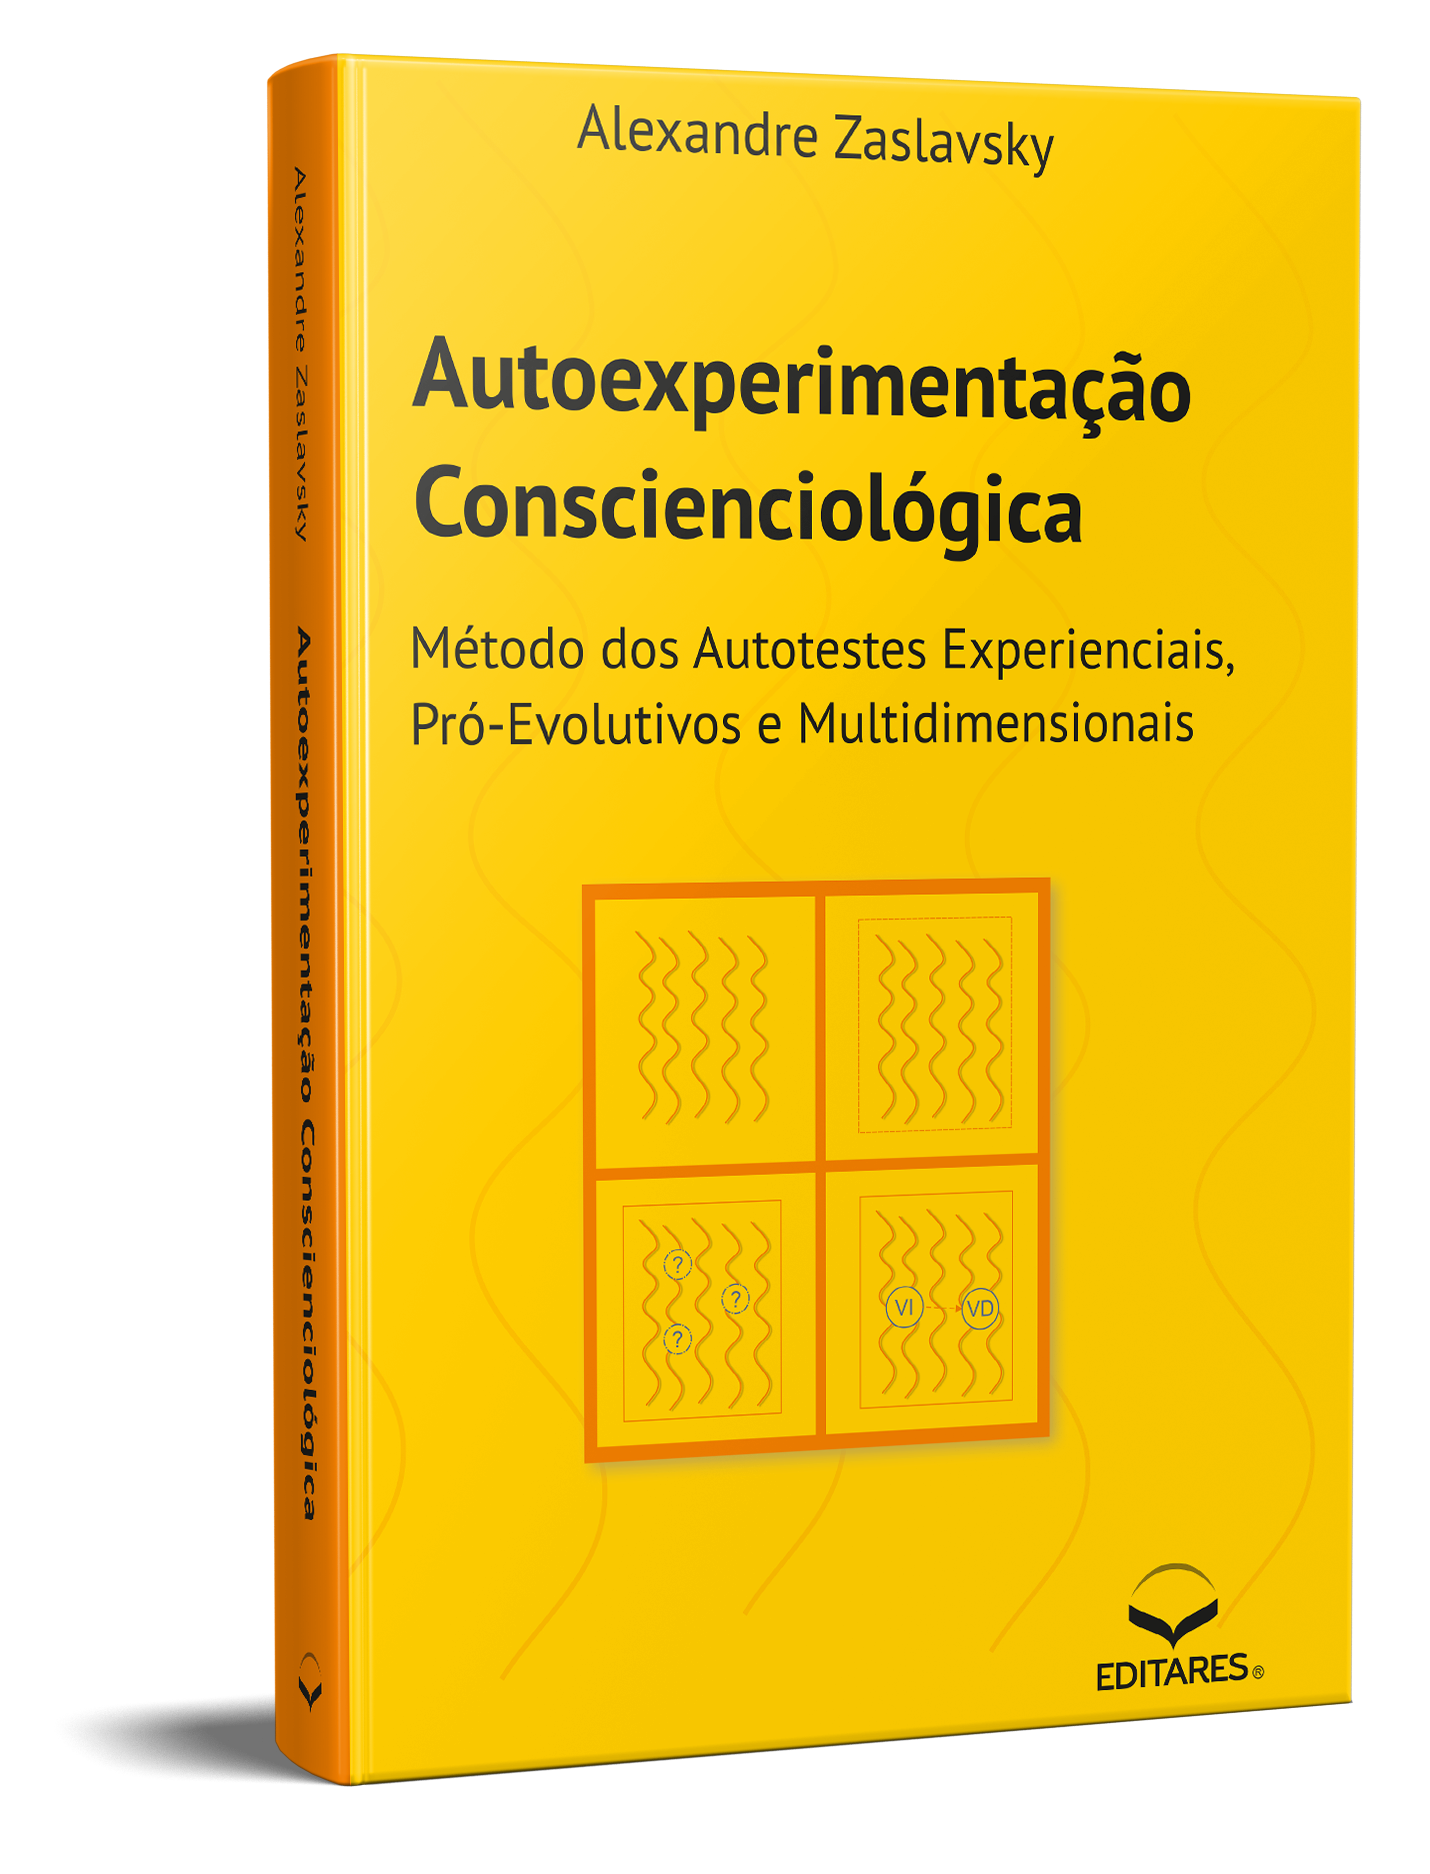
\includegraphics[width=4cm]{articles/entrevista/mockups/Alexandre-Zas.png}
\end{center}

\textbf{1. Qual foi a~motivação para a~escrita da obra? Por que a~definição deste tema para publicação de um livro?}

Desde que cheguei na Conscienciologia, o~seu novo paradigma científico, abrangendo a~multidimensionalidade dentre outros fatores, foi um grande motivador para mim. Assumi o~tema das bases da nova cientificidade conscienciológica, inicialmente de modo mais filosófico ou teórico e,~após, de modo mais conceitual e~teático. O~livro é~o~resultado dessas pesquisas sobre as bases teáticas da ciência Conscienciologia. A~autoexperimentação conscienciológica considero ser o~método científico mais básico e,~portanto, mais prioritário a~ser descrito, desenvolvido e~divulgado, tendo em vista o~público que se identifica com essa tarefa proexológica.

\textbf{2.       Quais foram as principais percepções, intra e~extrafísicas, durante a~pesquisa e~a~escrita da obra? E~posterior ao lançamento?}

A pesquisa e~escrita da obra foram muito ricas em autoexperimentos conscienciológicos, os quais são suscitados pelas experiências cotidianas e~são insitamente multidimensionais. A~interação com a~prática da tenepes também foi muito proveitosa, trazendo múltiplas inspirações de ideias, abordagens e~formulações mais assertivas interassistencialmente, seja diretamente com ideias ou indiretamente mediante parapercepções de processos extrafísicos. Foi possível observar na fase final da escrita o~aporte mais ostensivo de amparadores extrafísicos, auxiliando a~obter a~finalização propriamente da gescon, com a~qualidade necessária. Além disso, as trocas contínuas com colegas pesquisadores, mencionados nos Agradecimentos, foi de enorme auxílio ao longo da elaboração do trabalho.



\textbf{3.       Qual o~maior aprendizado com a~escrita desta obra?}

As revisões heterocríticas são imprescindíveis para a~qualificação do texto. Sem dúvida, considerar cuidadosamente as revisões recebidas, permitiu aprofundar e~amadurecer o~conteúdo do livro de modo incomparável com a~versão inicial. Além disso, a~publicação de uma obra tarística supõe a~assunção de autorresponsabilidade. Não é~possível depender da validação de autoridades para se trazer novas ideias a~público. O~autor chega a~determinado acúmulo de experiências e~conhecimentos que cabe tão somente a~ele, dentro dos parâmetros exigidos pela editora, assumir a~autoria publicamente. Portanto, o~primeiro maior aprendizado foi com a~interdependência e~o~segundo com a~independência relativa.


\textbf{4.       O~que poderia dizer como incentivo para que mais pesquisadores invistam na publicação de obras conscienciológicas?}

A escrita de uma obra conscienciológica é~uma oportunidade evolutiva inigualável. Desde a~escolha da temática, passando pelas experiências no decorrer da pesquisa e~escrita, até a~configuração final da obra, tudo isso expressa o~perfil específico do autor, conforme o~seu momento evolutivo. E~também, é~claro, atende ao grupo de afins que compartilha esse perfil. Além disso, apenas o~livro permite abordar as temáticas prioritárias no seu conjunto, de modo mais completo, seja na quantidade e~também na profundidade necessária. Publicar um livro enquanto gescon, portanto, é~possivelmente a~técnica evolutiva mais precisa e~eficaz.

\begin{pullquote}
``A escrita de uma obra conscienciológica é~uma oportunidade evolutiva inigualável.''
\end{pullquote}

        
    \end{multicols}
\end{document}
                           % Autoexperimentação Conscienciológica
    \documentclass{gescons}

\genre {Entrevista}
\author{Ricardo Rezende}
\title{Autoidentificação Proexológica}

\begin{document}
    \makeentrevistatitle
    \coverart{back/Ricardo_Rezende_Autoidentificao}

    \begin{multicols}{2}


%\noindent\includegraphics[width=9cm, height=10cm]{example-image} 
\begin{center}
    \includegraphics[width=8cm]{articles/entrevista/mockups/Ricardo-Rezende-Proexis.png}
\end{center}

\textbf{1. Qual foi a motivação para a escrita da obra? Por que a definição deste tema para publicação de um livro? }

A ideia de escrever esta obra surgiu em diálogo extrafísico com consciex amparadora, autorrememorada após o despertamento físico. A paraindicação dessa autogescon causou surpresa desconfortável porque não pensava em escrever livro com essa temática e estava priorizando outro trabalho gesconográfico. Apesar disso, desde jovem, confio, coopero com os amparadores extrafísicos e não pretendo mudar esse ortoposicionamento. Assim, acatei a paratarefa.

\begin{pullquote}
    ``A paraindicação dessa autogescon causou surpresa desconfortável porque não pensava em escrever livro nessa temática e estava priorizando outro trabalho gesconográfico''
\end{pullquote}

\textbf{2. Quais foram as principais percepções, intra e extrafísicas, durante a pesquisa e a escrita da obra? }

No decorrer da redação dos capítulos da obra, para a criação dos conteúdos, era necessário rever situações marcantes do próprio passado, ao modo de retrospectivação autobiográfica, relativas às memórias intermissivas e retrovidas pessoais. Nesse processo de revisão e análise de retrofatos particulares, constatava estar juntando, ordenando e encaixando no lugar certo as peças de complexo quebra-cabeças autoconscienciológico, sob os ângulos da \textit{Proexologia, Duplologia, Extrafisicologia, Intermissiologia e Holobiografologia.}

\textbf{3. Qual o maior aprendizado com a escrita desta obra? }

A compreensão aprofundada sobre a identificação e o desenvolvimento da autoproéxis.

\textbf{4. O que poderia dizer como incentivo para que mais pesquisadores invistam na publicação de obras conscienciológicas?}

O hábito da escrita conscienciológica com publicações seriadas resulta na ampliação dinâmica da hiperacuidade e na sustentação da conexão profícua com os amparadores extrafísicos e o holopensene homeostático da autoparaprocedência cursista, favorecendo o desenvolvimento intraconsciencial e da interassistencialidade tarística.

\begin{pullquote}
    ``O hábito da escrita conscienciológica com publicações seriadas resulta na ampliação dinâmica da hiperacuidade e na sustentação da conexão profícua com os amparadores extrafísicos e o holopensene homeostático da autoparaprocedência cursista.''
\end{pullquote}
    
    \end{multicols}
\end{document}


   % Autoidentificação Proexológica
    \documentclass{gescons}

\genre {Entrevista}
\author{Paula Gabriella Barbosa}
\title{Autoinversão Existencial: Compreensão e~Vivência}
\paginaurl{https://www.youtube.com/live/0akzpk8ifHI}

\begin{document}
    \makeentrevistatitle
    \coverart{back/Paula_Gabriela}

    \begin{multicols}{2}


%\noindent\includegraphics[width=9cm, height=10cm]{example-image} 

\begin{center}
    \includegraphics[width=7cm]{articles/entrevista/mockups/Paula}
\end{center}


\textbf{1. Qual foi a~motivação para a~escrita da obra? Por que a~definição deste tema para publicação de um livro?}

Minha principal motivação foi compartilhar aprendizados obtidos na aplicação prática da técnica da inversão existencial (invéxis), com o~objetivo de auxiliar os leitores na desdramatização dessa proposta evolutiva. O~título \textit{Autoinversão Existencial: Compreensão e~Vivência} reflete a~abordagem intraconsciencial adotada na obra, priorizando os efeitos evolutivos da técnica em detrimento de posturas pro forma. Busquei trazer uma visão mais realista e~experiencial, centrada na autorreflexão e~no autoenfrentamento cosmoético.

\begin{pullquote}
    ``O título Autoinversão Existencial: Compreensão e~Vivência reflete a~abordagem intraconsciencial adotada na obra, priorizando os efeitos evolutivos da técnica em detrimento de posturas pró forma.''
\end{pullquote}

\textbf{2. Quais foram as principais percepções, intra e~extrafísicas, durante a~pesquisa e~a~escrita da obra? E~posterior ao lançamento?}

Durante o~processo de escrita, percebi forte presença e~amparo de consciências extrafísicas com paravisual e~holopensene de matriz oriental, especialmente chinesa. Essa influência se manifestou tanto na leveza da abordagem quanto na clareza reflexiva do conteúdo, favorecendo o~desassédio pessoal e~o~da própria obra. Senti que a~escrita ocorreu em conjunto com os amparadores, dada a~rapidez e~fluidez da redação e~editoração. Considero que houve um investimento extrafísico significativo para que o~livro se materializasse neste momento evolutivo.

\begin{pullquote}
    ``Considero que houve um investimento extrafísico significativo para que o~livro se materializasse neste momento evolutivo.''
\end{pullquote}

\textbf{3. Qual o~maior aprendizado com a~escrita desta obra?}

O principal aprendizado foi compreender o~valor da escrita como forma de posicionamento multidimensional. Através deste livro, consegui expressar de maneira clara meu entendimento sobre a~técnica da invéxis, além de assumir um posicionamento mais lúcido diante do meu retrogrupo de base religiosa. Também entendi que, independentemente de onde eu esteja, a~obra continuará disponível para as consciências interessadas, mantendo vivas as ideias e~experiências compartilhadas.

\textbf{4. O~que poderia dizer como incentivo para que mais pesquisadores invistam na publicação de obras conscienciológicas?}

A escrita conscienciológica é~uma oportunidade de renovação da autoimagem, além de constituir um posicionamento multidimensional diante do tema abordado. Ao escrever, o~pesquisador amplia o~alcance assistencial de suas vivências e~reciclagens. Publicar é~uma forma de fixar marcos na própria trajetória e,~ao mesmo tempo, abrir caminhos para outras consciências.
    
    
    \end{multicols}
\end{document}




                      % Autoinversão Existencial
    \documentclass{gescons}

\genre {Entrevista}
\author{Luis Claudio Resende}
\title{Da Labilidade Parapsíquica A Assistencialidade Lúcida: Uma Trajetória Evolutiva}

\begin{document}
    \makeentrevistatitle
    \coverart{back/Luis_Claudio_Resende-Labilidade}

    \begin{multicols}{2}


%\noindent\includegraphics[width=9cm, height=10cm]{example-image} 
\begin{center}
    \includegraphics[width=8cm]{articles/entrevista/mockups/Luis_Claudio_Resende-Labilidade.png}
\end{center}

\textbf{1. Qual foi a motivação para a escrita da obra? Por que a definição deste tema para publicação de um livro? }

Após minha última viagem para a França houve a finalização de um ciclo específico de recomposição grupocármica.  Associado a esse fato havia um conjunto de experiências que poderiam servir de espelho para acelerar processos de resgate e acertos de outras consciências.

O tema principal é a evolução de um quadro de intensa labilidade para maior autocontrole energético e assistencial. 

Como autor e cobaia ao mesmo tempo desse laboratório, optei por escrever algo genuíno e acessível, tendo como público alvo os egressos de cursos intermissivos que tangenciassem a Conscienciologia.  Os relatos das experiências poderiam agir como atratores no processo de recuperação de CONS.

\textbf{2.       Quais foram as principais percepções, intra e extrafísicas, durante a pesquisa e a escrita da obra? E posterior ao lançamento?}

No meu caso específico houve conclusões de autopesquisa e relatos de experiências físicas e multidimensionais. Durante a confecção da obra ocorreu um estado de atividade mentalsomática mais evidente. Ela foi escrita em 60 dias. Optei por escrever da primeira à última página sem  revisar o texto, deixando o fluxo do pensamento mais livre. O resultado final, com ajustes pouco relevantes, deixou-me feliz. Era a minha  história , sob uma ótica mentalsomática, satisfazendo as expectativas iniciais.

\begin{pullquote}
    ``Durante a confecção da obra ocorreu um estado de atividade mentalsomática mais evidente.''
\end{pullquote}


\textbf{3.       Qual o maior aprendizado com a escrita desta obra?}

Foram dois grandes aprendizados:

\begin{itemize}
\item
  A conscin que mais ganha com a obra é aquela que escreve. Ter acesso a uma versão desassediada da sua pensenidade é algo muito interessante. Isso eleva as metas de suas pretensões evolutivas.
\item
  Vivenciando o grau de empenho e trabalho da equipe envolvida na edição, você aprende a valorizar mais o empenho tarístico de todo o grupo
\end{itemize}

\begin{pullquote}
    ``A conscin que mais ganha com a obra é aquela que escreve.''
\end{pullquote}


\textbf{4.       O que poderiam dizer como incentivo para que mais pesquisadores invistam na publicação de obras conscienciológicas?}

Apesar dos medos , contrafluxos , repercussões intra e extrafísicas negativas envolvendo uma gescon escrita , vale a pena seguir em frente porque , além de registrar e compartilhar o conhecimento, a obra per si chancela suas conquistas evolutivas. 



    


    \end{multicols}
\end{document}


     % Da Labilidade Parapsíquica
    \documentclass{gescons}

\genre {Entrevista}
\author{Ana Luiza Rezende e~Mabel Teles}
\authorrole{Organizadoras}
\title{Epicentrismo Consciencial: Casuísticas Recinológicas}
\paginaurl{https://www.youtube.com/live/yFrO2lGJzFo}

\begin{document}
    \makeentrevistatitle
    \coverart{back/Mabel_Teles_Ana_Luiza_Rezende}

    \begin{multicols}{2}

%\noindent\includegraphics[width=9cm, height=10cm]{example-image} 

\begin{center}
    \includegraphics[width=8cm]{articles/entrevista/mockups/Mabel-e-Ana-Luiza.png}
\end{center}

\subsubsection{1. Qual foi a~motivação para a~escrita da obra? Por que a~definição deste tema para publicação de um livro?}


O livro \textit{Epicentrismo Consciencial – Casuísticas Recinológicas} surgiu a~partir de uma sugestão do Prof. Waldo Vieira (1932--2015), em reunião do \textit{Conselho de Epicons} (CE), realizada no \textit{Hotel Interludium,} Foz do Iguaçu, em 2015. Na ocasião, ele propôs um levantamento das recins e~recéxis positivas e~exemplaristas já implementadas pelos integrantes do CE. A~obra é~fruto dessa proposta e~busca responder à~questão levantada no encontro: \textit{quais atos vêm qualificando o~epicentrismo de cada integrante do CE até agora? }

\subsubsection{2. Quais foram as principais percepções, intra e~extrafísicas, durante a~pesquisa e~a~escrita da obra? E~posterior ao lançamento?}

A obra, de cunho biográfico, possibilitou o~resgate de vivências significativas que contribuíram para o~desenvolvimento do epicentrismo de cada autor. O~registro de acertos e~reciclagens permitiu a~identificação de padrões evolutivos pessoais, fortalecendo a~responsabilidade perante a~grupalidade e~a~interassistência. A~publicação tem incentivado pesquisadores conscienciológicos a~aprofundarem as próprias reciclagens, visando à~qualificação do autepicentrismo e~o~aprimoramento da assistência multidimensional.  

\begin{pullquote}
``A obra, de cunha biográfico, possibilitou o~resgate de vivências significativas que contribuíram para o~desenvolvimento do epicentrismo de cada autor.''
\end{pullquote}


\subsubsection{3. Qual o~maior aprendizado com a~escrita desta obra?}

A escrita da obra permitiu o~aprofundamento da autopesquisas, além de ter demonstrado a~relevância da grupalidade na evolução pessoal, destacando como as interações, os desafios e~os aprendizados coletivos fortalecem o~epicentrismo de cada um. 


\subsubsection{4. O~que poderiam dizer como incentivo para que mais pesquisadores invistam na publicação de obras conscienciológicas?}

Publicar obras conscienciológicas é~uma forma de aprofundar a~autopesquisa, consolidar a~cognição evolutiva e~expandir a~interassistência. O~registro das experiências cria um legado evolutivo, beneficiando tanto o~autor quanto os leitores. Além disso, fortalece a~rede de pesquisadores e~contribui para a~ampliação do paradigma consciencial, estimulando novas reflexões e~descobertas.


\begin{pullquote}
``Publicar obras conscienciológicas é~uma forma de aprofundar a~autopesquisa, consolidar a~cognição evolutiva e~expandir a~interassistência.''
\end{pullquote}




    \end{multicols}
\end{document}















       % Epicentrismo Consciencial
    \documentclass{gescons}

\genre {Entrevista}
\author{Victor Bolfe}
\title{Estado Vibracional: 100 Perguntas e Respostas}

\begin{document}
    \makeentrevistatitle
    \coverart{back/Victor_Bolfe}

    \begin{multicols}{2}


\begin{center}
    \includegraphics[width=8cm]{articles/entrevista/mockups/Victor-Bolfe.png}
\end{center}

\textbf{1. Qual foi a motivação para a escrita da obra? Por que a definição deste tema para publicação de um livro?}

Aprofundar a pesquisa do EV de modo técnico, didático, detalhista, científico, profundo e exaustivo, deixando legado assistencial substancial para a humanidade. 

O tema foi definido por consolidar uma década de desenvolvimento da especialidade de pesquisa do autor sobre o Estado Vibracional. 

\textbf{2. Quais foram as principais percepções, intra e extrafísicas, durante a pesquisa e a escrita da obra? E posterior ao lançamento?}

O EV é tema básico nos estudos da Conscienciologia, porém ainda demanda muito esclarecimento e teática. Existe muito incentivo dos amparadores para a qualificação do EV por parte dos participantes da CCCI. 

\begin{pullquote}
    ``Existe muito incentivo dos amparadores para a qualificação do EV por parte dos participantes da CCCI.''
\end{pullquote}


\textbf{3. Qual o maior aprendizado com a escrita desta obra?}

Uma obra incialmente simples pode tomar grandes proporções caso o autor esteja aberto ao processo. 

\textbf{4. O que poderia dizer como incentivo para que mais pesquisadores invistam na publicação de obras conscienciológicas?}

A publicação de livro conscienciológico é oportunidade para materializar legado tarístico perpétuo, resultando em dividendos cármicos exponenciais ao longo do périplo evolutivo.

\begin{pullquote}
    ``A publicação de livro conscienciológico é oportunidade para materializar legado tarístico perpétuo.''
\end{pullquote}


    
    \end{multicols}
\end{document}
                        % Estado Vibracional
    \documentclass{gescons}

\genre {Entrevista}
\author{Pedro Borges}
\title{Etiologia: Teática Inversiva}

\begin{document}
    \makeentrevistatitle
    \coverart{back/Pedro_Borges}

    \begin{multicols}{2}

\begin{center}
    \vspace{-1cm}
    \includegraphics[width=6cm]{articles/entrevista/mockups/Pedro_Borges.png}
\end{center}

\vspace{-1cm}

\subsubsection{1.       Qual foi a motivação para a escrita da obra? Por que a definição deste tema para publicação de um livro?}

A motivação foi compreender melhor como conduzir as várias frentes da vida humana em conjunto e sempre em frente, mapeando o fluxo existencial do intermissivista ao assumir o desafio de vivenciar o pacote completo da Conscienciologia.

Para isso, valer-se de uma técnica evolutiva, no meu caso a inversão existencial, enquanto ferramenta para organização pessoal em prol da dinamização lúcida da evolução, é algo que ajuda bastante a concentrar o exclusivismo dos interesses pessoais na assistencialidade de modo mais otimizado.

A definição do tema enquanto Eitologia foi a forma mais eficaz e chamativa encontrada para se estudar a postura, atitude ou comportamento de levar tudo de eito, expressão coloquial bastante utilizada pelo prof. Waldo Vieira em suas aulas, debates e atendimentos, enquanto princípio fundamental para realização atacadista, a maior, da programação existencial, sem deixar nada para trás.

\subsubsection{2.       Quais foram as principais percepções, intra e extrafísicas, durante a pesquisa e a escrita da obra? E posterior ao lançamento?}

A motivação foi compreender melhor como conduzir as várias frentes da vida humana em conjunto e sempre em frente, mapeando o fluxo existencial do intermissivista ao assumir o desafio de vivenciar o pacote completo da Conscienciologia.

Para isso, valer-se de uma técnica evolutiva, no meu caso a inversão existencial, enquanto ferramenta para organização pessoal em prol da dinamização lúcida da evolução, é algo que ajuda bastante a concentrar o exclusivismo dos interesses pessoais na assistencialidade de modo mais otimizado.

% \begin{pullquote}
%     ``O que vai para o papel é uma expressão direta da consciencialidade do autor.''
% \end{pullquote}


\subsubsection{3.       Qual o maior aprendizado com a escrita desta obra?}

Complementando o que foi comentado na questão anterior, um dos grandes aprendizados foi o de verificar na prática o quanto a escrita de um livro conscienciológico é conscienciográfica, pois o que vai para o papel é uma expressão direta da consciencialidade do autor, sendo de grande relevância para a obra fazer sentido à própria verbação perante o que se deixou grafado.


\subsubsection{4.       O que poderia dizer como incentivo para que mais pesquisadores invistam na publicação de obras conscienciológicas?}

Escolha uma temática de interesse, busque bibliografia em todas as bases de consulta da Conscienciologia e comece a focar naquele assunto. Busque convergir as atividades para aquela temática, anote as experiências. Antes de começar a escrever, defina o escopo, a estrutura do livro e o público-alvo. E busque assessoria da Uniescon. Há várias atividades na IC para ajudar o autorando. 
    
Levar tudo de eito envolve não deixar nada para trás, e um dos pontos mais sérios desta condição é a publicação de obra conscienciológica, pois aciona um ponto de convergência entre várias áreas da vida, mexendo com a consciência como um todo. Nesse sentido, para o livro sair redondo, precisa-se desenvolver, não só a intelectualidade, mas também o parapsiquismo, a autopesquisa, a vida financeira, a parte afetiva, a liderança no voluntariado, entre outras variáveis. Tanto quem tem facilidade em escrever possui responsabilidade de compartilhar os achados pesquisísticos com teática, quanto aqueles que sentem dificuldade em colocar no papel possuem hoje condições de superar este travão e materializar a obra, com todos os recursos disponíveis na CCCI, ao modo de assessorias, cursos e editora especializada. Não desperdice, aproveite!

    \end{multicols}
\end{document}
                        % Etiologia
    \documentclass{gescons}

\genre {Entrevista}
\author{Karine Brito}
\title{Gratidão: Reconhecer, Expressar e~Retribuir}
\paginaurl{https://www.youtube.com/live/RN8tWr7Vk3c}

\begin{document}
    \makeentrevistatitle
    \coverart{back/Karine_Brito}

    \begin{multicols}{2}

\begin{center}
    \includegraphics[width=8cm]{articles/entrevista/mockups/Karine-Brito.png}
\end{center}

\textbf{1. Qual foi a~motivação para a~escrita da obra? Por que a~definição deste tema para publicação de um livro?}

A motivação para a~escrita do livro \textit{Gratidão: Reconhecer, Expressar e~Retribuir} foi a~descoberta de uma questão de saúde congênita em 2008, suscitando uma série de autorreflexões sobre a~vida, os vínculos conscienciais nutridos até então e,~sobretudo, o~subnível evolutivo quanto à~programação existencial.  A~doença foi um alerta consciencial para ampliar o~autodiscernimento, possibilitando identificar um grande travão evolutivo: a~ingratidão. A~escrita do livro surgiu como uma forma de retribuição lúcida das inúmeras benesses recebidas nesse processo. A~inspiração extrafísica era explicitar como se dá o~desenvolvimento da cognição sobre a~gratidão, incentivando o~seu cultivo autoconsciente no dia a~dia. 

\begin{pullquote}
``A doença foi um alerta consciencial para ampliar o~autodiscernimento, possibilitando identificar um grande travão evolutivo: a~ingratidão.''
\end{pullquote}

\textbf{2. Quais foram as principais percepções, intra e~extrafísicas, durante a~pesquisa e~a~escrita da obra? E~posterior ao lançamento?}

Ao longo dos 16 anos de pesquisa e~escrita desta obra percebi de modo ostensivo a~atuação dos amparadores, intra e~extrafísicos. Muitos amigos evolutivos acompanharam de perto o~desenvolvimento da pesquisa, ajudando nas autorreflexões, nos debates sobre o~tema e~nas revisões. Durante a~escrita do livro, desde o~início tive muitas inspirações da equipex. Percebia um interesse genuíno dos amparadores em materializar esta publicação, destacando a~sua relevância no momento evolutivo atual. A~principal inspiração extrafísica foi apresentar, de modo técnico e~didático, a~gratidão como base da recomposição grupocármica. Posterior ao lançamento, me chamou a~atenção a~assistência a~ouvintes de curso intermissivo ligados à~invéxis, muito atentos ao tema da gratidão.

\begin{pullquote}
``Percebia um interesse genuíno dos amparadores em materializar esta publicação, destacando a~sua relevância no momento evolutivo atual.''
\end{pullquote}

\textbf{3. Qual o~maior aprendizado com a~escrita desta obra?}

O maior aprendizado com a~escrita desta obra foi, sem dúvida, levar a~sério o~alerta consciencial proexológico, colocando a~recomposição grupocármica como prioridade. Isso foi a~mola propulsora evolutiva para desenvolver a~gratidão. 

\textbf{4. O~que poderia dizer como incentivo para que mais pesquisadores invistam na publicação de obras conscienciológicas?}

A obra conscienciológica é~retribuição fundamental do intermissivista, favorecendo o~autorrevezamento lúcido e~a~ampliação da interassistencialidade tarística a~partir da recin do autor. Se você melhorou, ajude outras pessoas a~chegarem até lá! 
    
    
    \end{multicols}
\end{document}



                        % Gratidão
    \documentclass{gescons}

\genre {Entrevista}
\author{Roberta Bouchardet}
\title{Interassistência: Teoria e~Prática Sob a~Ótica da Conscienciologia}
\paginaurl{https://www.youtube.com/live/zasm7A2swDQ}

\begin{document}
    \makeentrevistatitle
    \coverart{back/Roberta_Bouchardet}

    \begin{multicols}{2}

\begin{center}
    \includegraphics[width=7cm]{articles/entrevista/mockups/Roberta-Bouchardet}
\end{center}

%\begin{center}
%    \includegraphics[width=8cm]{articles/entrevista/mockups/Roberta-Bouchardet}
%\end{center}

\textbf{1.       Qual foi a~motivação para a~escrita da obra? Por que a~definição deste tema para publicação de um livro?}

Sempre gostei de livros e~de escrever. E~assim, junto com o~incentivo do Prof. Waldo em deixar uma gestação consciencial nessa existência, veio a~motivação de registrar parte do conhecimento adquirido em tantas décadas de estudo e~autopesquisas na Conscienciologia. A~definição do tema veio aos poucos. Começou com o~verbete Autoamparo, que deveria ser a~base do livro, mas a~temática cresceu e~se tornou Interassistência, sendo o~Autoamparo um dos capítulos do livro.

\textbf{2.       Quais foram as principais percepções, intra e~extrafísicas, durante a~pesquisa e~a~escrita da obra? E~posterior ao lançamento?}

Já há alguns anos eu estava escrevendo alguns capítulos, sem saber ainda o~escopo da obra, e~no Acoplamentarium de pesquisa, durante uma prática energética, tive o~fenômeno de captação de ideias e~visualizei todo o~sumário, os capítulos a~serem escritos. Anotei tudo e~a~partir daí a~escrita fluiu bem mais rapidamente. Durante a~escrita, sentia-me muito motivada e~energizada, o~mentalsoma não cansava. O~que cansava era o~soma, que exigia parar. Após o~lançamento, percebo mudanças pensênicas, maior tranquilidade, talvez novos amparadores, o~que está em avaliação ainda.

\begin{pullquote}
    ``Durante a~escrita, me sentia muito motivada e~energizada, o~mentalsoma não cansava''
\end{pullquote}


\textbf{3.       Qual o~maior aprendizado com a~escrita desta obra?}

Aprendi muito sobre o~processo de organização de uma obra para publicação. Uma coisa é~escrever textos para nós mesmos ou trabalhos para cursos. Outra, muito diferente, é~o~livro. Muitas etapas são necessárias e~muitas pessoas são envolvidas e~trabalham arduamente junto com o~autor. Durante o~processo, tornei-me participante do Conselho Editorial da Editares e~busco auxiliar outros autores nesse processo. É~preciso persistência e~paciência; a~pressa em fazer rápido acaba assediando o~fluxo e~atrasando mais ainda os trabalhos. É~preciso trabalhar ombro a~ombro, tanto com os amparadores extrafísicos, como também com os colegas intrafísicos nas várias etapas de edição do livro. Entrar em conflito é~contraproducente.

\begin{pullquote}
    ``É preciso persistência e~paciência; a~pressa em fazer rápido acaba assediando o~fluxo e~atrasando mais ainda os trabalhos.''
\end{pullquote}

\textbf{4.       O~que poderia dizer como incentivo para que mais pesquisadores invistam na publicação de obras conscienciológicas?}

Escolha uma temática de interesse, busque bibliografia em todas as bases de consulta da Conscienciologia e~comece a~focar naquele assunto. Busque convergir as atividades para aquela temática, anote as experiências. Antes de começar a~escrever, defina o~escopo, a~estrutura do livro e~o~público-alvo. E~busque assessoria da Uniescon. Há várias atividades na IC para ajudar o~autorando. 
    
    
    \end{multicols}
\end{document}
                  % Interassistência
    \documentclass{gescons}

\genre {Entrevista}
\author{Michel Chad}
\title{Megapensenes Trivocabulares Pró-evolutivos}
\paginaurl{https://www.youtube.com/live/lyb7pNbQWh0}

\begin{document}
    \makeentrevistatitle
    \coverart{back/Michel_Chad}

    \begin{multicols}{2}


%\noindent\includegraphics[width=9cm, height=7cm]{example-image} 

\begin{center}
    \includegraphics[width=8cm]{articles/entrevista/mockups/Michel-Chad.png}
\end{center}

\textbf{1.       Qual foi a motivação para a escrita da obra? Por que a definição deste tema para publicação de um livro?}

Sou voluntário do IIPC desde 1996. Desde que Waldo Vieira apresentou esta técnica em um curso avançado ministrado em São Paulo, comecei a estudar os megapensenes trivocabulares e elaborar meus próprios. 

Nesta época participava do \textit{Grupo de Pesquisa da Conscienciologia} (GPC) do livro de Waldo Vieira,  \textit{700 Experimentos da Conscienciologia.} Tínhamos encontros semanais de estudo prévio de 2 capítulos do tratado e, na reunião, criávamos uma pensata sobre cada um dos capítulos. Posteriormente, o desafio era formular uma nova frase síntese juntando as duas anteriores. Diversas vezes criamos megapensenes trivocabulares nesta tarefa. 

Talvez pela minha formação em Engenharia Química, o processo de confecção das pensatas trivocabulares e suas 200 fórmulas apresentadas no
\textit{Manual de Megapensenes Trivocabulares,} de Waldo Vieira,  fascinou-me. Pela leitura crítica deste material, busquei aprender e utilizar, na confecção dos meus megapensenes, todas as fórmulas descritas. Inclusive no meu livro proponho 6 fórmulas inéditas criadas por mim.

Outra gescon que serviu como modelo  para minha obra, foi o livro \textit{Megapensenes Trivocabulares da Interassistencialidade,} de Aline Niemeyer, publicado em 2016.

Participei do curso Técnica de Mais 1 ano de Vida Intrafísica, em 2016 e 2017,  ministrado pelo CEAEC, no qual uma das minhas metas foi a escrita e publicação de uma obra com megapensenes trivocabulares. Meta finalmente cumprida em 2024.

\textbf{2.       Quais foram as principais percepções, intra e extrafísicas, durante a pesquisa e a escrita da obra? E posterior ao lançamento?}

Penso que entre as gescons que me propus no meu curso intermissivo, uma delas está relacionada com a produção de neopensatas trivocabulares. 

\begin{pullquote}
    ``Penso que entre as gescons que me propus no meu curso intermissivo, uma delas está relacionada com a produção de neopensatas trivocabulares.''
\end{pullquote}

\textbf{3.       Qual o maior aprendizado com a escrita desta obra?}

Cito entre os benefícios no estudo e elaboração dos megapensenes trivocabulares: ampliação dos diversos dicionários cerebrais, inclusive o analógico; aprimoramento do atributo da associação de ideias; aprofundamento no pensar; comunicação interassistencial sintética; criação do hábito de compor sínteses; desassédio mental; desenvolvimento da criticidade; facilitação da criação e compreensão de neologismos; flexibilidade pensênica; hábito das ponderações das verpons; indução da criatividade.


\textbf{4.       O que poderia dizer como incentivo para que mais pesquisadores invistam na publicação de obras conscienciológicas?}

Finalizo agradecendo a todas as consciências envolvidas neste projeto sugerindo aos interessados estudarem a fundo as 200 fórmulas apresentadas no livro e desenvolverem os seus próprios megapensenes trivocabulares. Elabore neopensatas trivocabulares.


\begin{pullquote}
``Elabore neopensatas trivocabulares.''
\end{pullquote}
    
    \end{multicols}
\end{document}


                         % Megapensenes Trivocabulares
    \documentclass{gescons}

\genre {Entrevista}
\author{Virginia Ruiz}
\title{Migrações Proexológicas Internacionais: Holocarma das Nações \& Acertos Grupocármicos}
\paginaurl{https://www.youtube.com/live/r2iDY1MbxRY}

\begin{document}
    \makeentrevistatitle
    \coverart{back/Virginia}

    \begin{multicols}{2}


\begin{center}
    \includegraphics[width=8cm]{articles/entrevista/mockups/Virginia}
\end{center}


\textbf{1.       Qual foi a~motivação para a~escrita da obra? Por que a~definição deste tema para publicação de um livro?}

A motivação principal foi doar meu laboratório consciencial como voluntária internacional que migrou de Madri, Espanha, a~Foz do Iguaçu, Brasil, para participar da maxiproéxis grupal. Além disso, contribuir para a~internacionalização da Conscienciologia, trazendo neoideias e~reflexões sob a~ótica do holocarma das nações e~do Universalismo.


\textbf{2.       Quais foram as principais percepções, intra e~extrafísicas, durante a~pesquisa e~a~escrita da obra? E~posterior ao lançamento?}

Vivenciei percepções marcantes, a~exemplo do investimento paciente da equipin e~equipex, projeções lúcidas sobre a~materialização do livro e~a~identificação do público-alvo de proexistas internacionais e~migrantes intermissivistas. Senti também maior compromisso com a~interassistência tarística ao redor do mundo. Após o~lançamento, percebi expansão da lucidez pensênica e~maior abertura intraconsciencial.


\textbf{3.       Qual o~maior aprendizado com a~escrita desta obra?}

O livro me mostrou que a~migração pode ser entendida como estratégia autoevolutiva capaz de potencializar a~maxiproéxis internacional. Ao mesmo tempo, evidenciou, na prática, o~significado do Universalismo por meio da interação e~convivência com conscins de diversas culturas e~idiomas, ampliando a~compreensão da responsabilidade holocármica migratória e~demandando novos posicionamentos cosmoéticos perante grupos de retrovidas e~reciclagens intraconscienciais.

\begin{pullquote}
    ``O livro me mostrou que a~migração pode ser entendida como estratégia autoevolutiva capaz de potencializar a~maxiproéxis internacional.''
\end{pullquote}

\textbf{4.       O~que poderia dizer como incentivo para que mais pesquisadores invistam na publicação de obras conscienciológicas?}

Animo todos a~escreverem sobre sua própria teática pessoal, pois esse movimento torna a~conscin exemplarista cosmoética diante do grupo intra e~extrafísico. Em última análise, final, trata-se de assumir a~responsabilidade intermissiva que nos aproxima da compléxis e~amplia nosso papel evolutivo nestes tempos de reurbex. E~você, leitor, o~que falta para compartilhar seus achados autopesquisísticos?


\begin{pullquote}
    ``Em última análise, final, trata-se de assumir a~responsabilidade intermissiva que nos aproxima da compléxis e~amplia nosso papel evolutivo nestes tempos de reurbex.''
\end{pullquote}

    
    \end{multicols}
\end{document}
                            % Migrações Proexológicas
    \documentclass{gescons}

\genre {Entrevista}
\author{Luimara Schmit}
\title{Mutatis Mutandis: Teoria e~Prática da Reciclagem Existencial}
\paginaurl{https://www.youtube.com/live/FXWtZpHxP8k}

\begin{document}
    \makeentrevistatitle
    \coverart{back/Luimara_Schmit}

    \begin{multicols}{2}

\begin{center}
    \includegraphics[width=6cm]{articles/entrevista/mockups/Luimara.png}
\end{center}

\textbf{1. Qual foi a~motivação para a~escrita da obra? Por que a~definição deste tema para publicação de um livro?}


O tema principal do livro é~a~\emph{reciclagem existencial,} técnica conscienciológica que objetiva a~mudança para melhor dos aspectos da vida humana e~interdimensional para quem estiver predisposto a~adotar novo conjunto de valores pró-evolutivos.

A primeira seção, composta por perguntas e~respostas, propicia a~ampliação do conhecimento teórico sobre recéxis, enquanto a~segunda seção oportuniza a~autopesquisa prática, contendo 100 perguntas para a~recexometria mais ampla. Para o~autodiagnóstico mais assertivo é~apresentado o~\emph{Recexograma,} no formato de planilha. Assim, os interessados têm a~possibilidade de aprofundar a~compreensão do tema e~se instrumentalizarem para a~aplicação didática da recéxis.

Identifico que o~gosto pela leitura e~a~afinidade com a~escrita são inatos. Reconheço que o~incentivo e~o~exemplarismo do professor Waldo Vieria, associados à~compreensão do potencial interassistencial e~de autorrevezamento multiexistencial de uma gescon, foram os propulsores para as autorrenovações essenciais à~dedicação para a~escrita do livro.

A escolha do tema relacionado à~\emph{reciclagem existencial} tem relação com as vivências e~as necessidades pessoais identificadas enquanto intermissivista, conscienciômetra e~aplicante da \emph{técnica da recéxis} há mais de duas décadas.

Tendo em vista que não dispunha de instrumento específico, elaborei o~\emph{Programa de Recéxis,} incluindo o~\emph{Recexograma} (composto por 100 itens para auxiliar no acompanhamento da performance pessoal nas diversas áreas da vida) e~o~\emph{Plano de Ação Recexométrico.} Desse modo, a~partir do programa de autorrenovações continuadas, pautado na proposta de reciclagem prazerosa, possibilita-se a~conquista do autoequilíbrio holossomático, alinhado aos objetivos de alcançar a~desperticidade e~o~completismo existencial.

\textbf{2. Quais foram as principais percepções, intra e~extrafísicas, durante a~pesquisa e~a~escrita da obra?}

Percebi a~diversificação e~o~aumento de demandas assistenciais familiares, profissionais e~no voluntariado, sinalizando a~checagem da sustentabilidade pessoal afim aos temas pesquisados. Do ponto de vista multidimensional, observei a~sutilização do parapsiquismo, o~crescendo gradual das parapercepções e~a~ampliação da captação de inspirações, a~partir da maior conexão com o~amparador de função. O~título principal, \emph{Mutatis Mutandis,} foi inspirado extrafisicamente na tenepes e~complementou de modo instigante a~abordagem teática à~recéxis.

\textbf{3. Qual o~maior aprendizado com a~escrita desta obra?}

O aumento da \emph{autoconscientização multidimensional,} incluindo inusitado rol de sincronicidades, está contribuindo para a~ampliação do autorrealismo e~a~sensação de \emph{ser consciência.} Compreendi, na prática, que a~escrita conscienciológica é~teática e~requer exemplarismo. Também propicia a~qualificação de habilidades interassistenciais e~do respeito interconsciencial, pois cada qual estabelece o~ritmo e~o~limite para as autorreciclagens.

\textbf{4. O~que poderia dizer como incentivo para que mais pesquisadores invistam na publicação de obras conscienciológicas?}

Compartilhe suas experiências!

Elaborar \emph{gestação consciencial} sob a~perspectiva do neoparadigma é~desafiador e~gratificante. O~livro é~um \emph{investimento evolutivo} muito significativo e~pode oportunizar a~catalisação de recomposições grupocármicas insuspeitas.

% \begin{pullquote}
% ``Elaborar gestação consciencial sob a~perspectiva do neoparadigma é~desafiador e~gratificante.''
% \end{pullquote}
% 
    
    \end{multicols}
\end{document}



                      % Mutatis Mutandis
    \documentclass{gescons}

\genre {Entrevista}
\author{Cristina Bassanesi}
\title{O Calidoscópio da Evolução Consciencial: Abordagem Interparadigmática da Evoluciologia}


\begin{document}
    \makeentrevistatitle
    \coverart{back/Cristina_Bassanesi}

    \begin{multicols}{2}

\textbf{Qual foi a motivação para a escrita da obra? Por que a definição deste tema para publicação de um livro?}

Esta obra teve como motivação escrever sobre a \textit{Mutabilidade Consciencial Não Linear,} tema pertinente à \textit{Especialidade Evoluciologia,} empregando abordagem científica, multidisciplinar e interparadigmática.

A definição pelo tema somente foi estabelecida em definitivo após o movimento pessoal de começar a escrever. O roteiro previamente delineado mudou logo no início, quando ampliei a cosmovisão sobre o que poderia ser o tema central do livro e passei a aplicar \textit{o princípio de os fatos e parafatos orientarem a pesquisa.}

\textbf{Quais foram as principais percepções, intra e extrafísicas, durante a pesquisa e a escrita da obra? E posterior ao lançamento?}

Atitude pessoal determinante para manter a rotina de escrita foi o autoposicionamento de priorizar 1 turno fixo do dia (manhã) para à escrita, em detrimento dos inúmeros apelos para envolvimento em outras atividades. Nesse ponto, a sobreveniência do desassédio mentalsomático e a parapercepção do amparo de função, atuando tanto com inspirações quanto no auxílio à resolução de entraves dos mais variados tipos tornou-se evidente.

As repercussões favoráveis do livro publicado trouxeram grande alegria, porém, com maior intensidade, asseveraram o autocompromisso intermissivo com a tares autoral. 

\begin{pullquote}
``As repercussões favoráveis do livro publicado trouxeram grande alegria, porém, com maior intensidade, asseveraram o autocompromisso intermissivo com a tares autoral.''
\end{pullquote}

\textbf{Qual o maior aprendizado com a escrita desta obra?}

Sem dúvida, a conclusão da obra deixou saldo de aprendizados, dentre os quais destaco o valor do exercício da persistência e paciência na sustentação gesconográfica. Aprendizado adicional foi o de eliminar o apego a ideias, frases e até vocábulos, que a princípio podem soar muito boas. Contudo, por vezes, atravancam durante horas ou dias a fluidez da escrita. A sugestão é guardá-las em algum arquivo próprio, para utilização em outra oportunidade. 

\begin{pullquote}
``Sem dúvida, a conclusão da obra deixou saldo de aprendizados, dentre os quais destaco o valor do exercício da persistência e paciência na sustentação gesconográfica.''
\end{pullquote}

\textbf{O que poderia dizer como incentivo para que mais pesquisadores invistam na publicação de obras conscienciológicas?}

Deixo o incentivo, aos potenciais escritores, a investirem na escrita de obras conscienciológicas, expondo as autossingularidades ou especialidades pessoais, as quais podem trazer novos vieses de compreensão sobre a evolução consciencial e novas senhas aos neointermissivistas. 

    %\noindent\includegraphics[width=11cm, height=12cm]{example-image} 

\begin{center}
    \includegraphics[width=8cm]{articles/entrevista/mockups/Cristina-Bassanesi.png}
    %\noindent\includegraphics[width=8cm, height=10cm]{example-image}
\end{center}
    
    \end{multicols}
\end{document}
                  % O Calidoscópio da Evolução
    \documentclass{gescons}

\genre {Entrevista}
\author{Ricardo Rezende}
\title{Ortoprincípios Norteadores da Invéxis}

\begin{document}
    \makeentrevistatitle
    \coverart{back/Ricardo_Rezende_Ortoprincipios}

\begin{center}
    \includegraphics[width=7cm]{articles/entrevista/mockups/Ricardo-Rezende-Invexis.png}
\end{center}

    \begin{multicols}{2}


%\noindent\includegraphics[width=9cm, height=9cm]{example-image} 

\textbf{1. Qual foi a motivação para a escrita da obra? Por que a definição deste tema para publicação de um livro?}

Desde junho de 2022, este autor iniciou a escrita de verbetes a respeito de temas de Invexologia, incentivado pelo início dos trabalhos voluntários pessoais na Assinvéxis. Nesse período, houve imersão ou saturação intelectiva homeostática quanto aos conteúdos sobre inversão existencial, por meio da dedicação à verbetografia, resultando no estudo do tema \textit{holofilosofia da invéxis}.

Mais adiante para compreender melhor o assunto, iniciou-se mapeamento para identificar quais princípios cosmoéticos ou as \textit{condições evoluídas de se viver} poderiam compor a filosofia teática da inversão existencial. Para isso, realizou-se pesquisas em publicações conscienciológicas buscando localizar nos fundamentos ou nas bases teórico-práticas da Invexologia os ortoprincípios constituintes, de modo a estruturar a tese central da obra \textit{Ortoprincípios Norteadores da Invéxis}.

Portanto, essa obra advém da curiosidade pesquisística e determinação grafopensênica com o propósito de descortinar a filosofia teática da invéxis, sob 
o ângulo interdisciplinar de 5 especialidades: Principiologia, Experienciologia, Traforologia, Evoluciologia e Seriexologia.

\begin{pullquote}
``Essa obra advém da curiosidade pesquisística e determinação grafopensênica com o propósito de descortinar a filosofia teática da invéxis.''    
\end{pullquote}




\textbf{2. Qual o maior aprendizado com a escrita desta obra?}

A compreensão aprofundada da holofilosofia da invéxis, a expansão da paracognição invexológica e da lucidez invexometrológica pessoal.

\textbf{3. O que poderiam dizer como incentivo para que mais pesquisadores invistam na publicação de obras conscienciológicas?}

O hábito da escrita conscienciológica com publicações seriadas resulta na ampliação dinâmica da hiperacuidade e na sustentação da conexão profícua com os amparadores extrafísicos e o holopensene homeostático da autoparaprocedência cursista, favorecendo o desenvolvimento intraconsciencial e da interassistencialidade tarística.


    
    
    \end{multicols}


\end{document}

      % Ortoprincípios Norteadores
    \documentclass{gescons}

\genre {Entrevista}
\author{Ana Mazzonetto}
\title{Retomada de Tarefa: Reencontro com o~Paradever Intermissivo}
\paginaurl{https://www.youtube.com/live/9A6h__c2uxk}

\begin{document}
    \makeentrevistatitle

\coverart{back/ana_mazzonetto}

    \begin{multicols}{2}


\begin{center}
%\noindent\includegraphics[width=8cm, height=10cm]{example-image}

    \includegraphics[width=8cm]{articles/entrevista/mockups/Ana-Mazzonetto}
\end{center}

\subsubsection{1. Qual foi a~motivação para a~escrita da obra? Por que a~definição deste tema para publicação de um livro?}

O livro é~fruto de demanda extrafísica, portanto a~maior motivação foi o~próprio convite mesmo. 

Desde o~ano de 2020, o~foco pesquisístico estava voltado ao tema do “antiassoberbamento”. Estava em curso projeto para a~escrita de livro sobre o~tema. Todavia, em 10 de julho de 2022, após a~conclusão da técnica da tenepes, sobreveio convite, por parte de amparadores extrafísicos, para a~escrita e~publicação de livro conscienciológico acerca da retomada de tarefa. 

A clareza da demanda extrafísica não deixou dúvidas sobre a~importância do tema. Desde então, a~pesquisa e~a~produção gesconográfica voltaram-se ao entendimento teático da temática.

\subsubsection{2. Quais foram as principais percepções, intra e~extrafísicas, durante a~pesquisa e~a~escrita da obra? E~posterior ao lançamento?}

Durante a~escrita da obra, vivenciei muitos acoplamentos mentaissomáticos com os amparadores, tanto nas fases de escrita, quanto de pesquisa, formulação de hipóteses e~reflexões plasmadas no livro. 

Parecia que tudo que enxergava tinha relação com a~temática, foi experiência muito legal de hiperfoco. Verifiquei também o~aumento gradativo do público-alvo interassistencial.

Após o~lançamento, a~principal percepção foi de aumento da responsabilidade interassistencial. 

\subsubsection{3. Qual o~maior aprendizado com a~escrita desta obra?}

Aprendi a~valorizar meus trafores, sem eles o~livro não teria saído do campo das ideias. Compreendi também o~alcance interassistencial da autaceitação da história pessoal.

\begin{pullquote}
``Compreendi também o~alcance interassistencial da autaceitação da história pessoal''
\end{pullquote}


\subsubsection{4. O~que poderia dizer como incentivo para que mais pesquisadores invistam na publicação de obras conscienciológicas?}

Escolha o~tema de seu livro, invista na qualificação recinológica e~gesconográfica e~só pare quando o~livro estiver pronto, simples assim. 

Ouse escrever, intermissivista!

\begin{pullquote}
``Escolha o~tema de seu livro, invista na qualificação recinológica e~gesconográfica e~só pare quando o~livro estiver pronto, simples assim.''
\end{pullquote}



    
    \end{multicols}
\end{document}
                      % Retomada de Tarefa
    
    \genre{}
    \title {Balanço}
    \author{}
    \authorrole{}
    \makecovertitle{articles/fundo-generico.png}{}
    \documentclass{gescons}

\genre {Balanço}
%\author{Ricardo Rezende}
%\roles{Voluntário do Setor Comercial da Editares}
\title{Balanço da Editares 21 Anos}



\begin{document}
    \makeentrevistatitle
    %\maketitle

    %\fullwidthimage{fields}{b}

    %\coverart{back/editorial}
    \coverart{../fundo-generico.png}
    
    
\begin{center}
    
    \includegraphics[height=5.8cm]{articles/balanco/grafico/balanco1.png} 
    \includegraphics[height=5.8cm]{articles/balanco/grafico/balanco2.png}  
    \includegraphics[height=5.8cm]{articles/balanco/grafico/balanco3.png}  
    \includegraphics[height=7cm]{articles/balanco/grafico/balanco4.png}  

\end{center}
    
%\begin{center}
%    \includegraphics[width=9cm]{articles/atualizacoes/fotos/escola-editores/escola-editores1.jpeg} 
%\end{center}


%    \end{multicols}
\end{document}



    %\documentclass{gescons}

\genre {Editorial}
\title {Hello world}
\author{Abdullah José Kim}

\begin{document}
    \maketitle

    \fullwidthimage{fields}{b}

    \begin{multicols}{3}
        \begin{lead}
            \lipsum[1]
        \end{lead}

        \lipsum[2-3]
        
        \begin{pullquote}
            ``If you cannot do great things, do small things in a~great way.'' amanda
        \end{pullquote}
        
        \lipsum[4]
        
    \end{multicols}
\end{document}

    %\documentclass{gescons}

\genre {Science}
\title {Engineer becomes famous after building first-ever PUNDITECTOR}
\author{Fanny Furling}

\begin{document}
    \maketitle
    
    \begin{lead}
        \lipsum[1]
    \end{lead}
    
    \begin{multicols}{3}
        \lipsum[2-11]
    \end{multicols}
    
    \begin{figure}
        \includegraphics[width=\textwidth]{landscape}
    \end{figure}
\end{document}

    %\documentclass{gescons}

\genre {Economy}
\title {Retired fundamentalists infuriated by government's decision to declare total workfare}
\author{Kane Keynes}

\begin{document}
    \maketitle

    
    
    
    \begin{multicols}{2}
        \begin{lead}
            \lipsum[1]
        \end{lead}

        \lipsum[2]
        
        \includegraphics[width=\columnwidth]{landscape}
        
        \lipsum[3-6]
    \end{multicols}
\end{document}

    %\documentclass{gescons}

\genre {Feature story}
\title {Is broccoli from outer space?}
\author{Dwight Greenman}

\begin{document}
    \makecovertitle{broccoli}{\lipsum[1]}

    \begin{multicols}{3}

        \lipsum[2-8]
        
        \lipsum[9-18]
        
        No.
    \end{multicols}
\end{document}

    
    %\genre {Anuncio}
    %\fullpageadvertisement{images/amigos-da-enciclopedia}{10}{10}
\end{document}
